\documentclass{article}
\usepackage[a4paper,top=2.5cm,bottom=2.5cm,left=2.5cm,right=2.5cm]{geometry}
\usepackage{makeidx}
\usepackage{natbib}
\usepackage{graphicx}
\usepackage{multicol}
\usepackage{float}
\usepackage{listings}
\usepackage{color}
\usepackage{ifthen}
\usepackage[table]{xcolor}
\usepackage{textcomp}
\usepackage{alltt}
\usepackage{ifpdf}
\ifpdf
\usepackage[pdftex,
            pagebackref=true,
            colorlinks=true,
            linkcolor=blue,
            unicode
           ]{hyperref}
\else
\usepackage[ps2pdf,
            pagebackref=true,
            colorlinks=true,
            linkcolor=blue,
            unicode
           ]{hyperref}
\usepackage{pspicture}
\fi
\usepackage[utf8]{inputenc}
\usepackage{mathptmx}
\usepackage[scaled=.90]{helvet}
\usepackage{courier}
\usepackage{sectsty}
\usepackage{amssymb}
\usepackage[titles]{tocloft}
\usepackage{doxygen}
\lstset{language=C++,inputencoding=utf8,basicstyle=\footnotesize,breaklines=true,breakatwhitespace=true,tabsize=4,numbers=left }
\makeindex
\setcounter{tocdepth}{3}
\renewcommand{\footrulewidth}{0.4pt}
\renewcommand{\familydefault}{\sfdefault}
\hfuzz=15pt
\setlength{\emergencystretch}{15pt}
\hbadness=750
\tolerance=750
\begin{document}
\hypersetup{pageanchor=false,citecolor=blue}
\begin{titlepage}
\vspace*{7cm}
\begin{center}
{\Large Un\-Banco \\[1ex]\large 1.\-3 }\\
\vspace*{1cm}
{\large Generated by Doxygen 1.8.3.1}\\
\vspace*{0.5cm}
{\small Sun Jul 14 2013 11:26:02}\\
\end{center}
\end{titlepage}
\pagenumbering{roman}
\tableofcontents
\pagenumbering{arabic}
\hypersetup{pageanchor=true,citecolor=blue}
\section{Hierarchical Index}
\section{Class Hierarchy}
This inheritance list is sorted roughly, but not completely, alphabetically\-:\begin{DoxyCompactList}
\item \contentsline{section}{Account}{\pageref{d7/d10/classAccount}}{}
\item \contentsline{section}{Main\-Interface}{\pageref{d2/da2/classMainInterface}}{}
\begin{DoxyCompactList}
\item \contentsline{section}{Main\-Adm\-Menu}{\pageref{d9/d86/classMainAdmMenu}}{}
\item \contentsline{section}{Main\-Cus\-Menu}{\pageref{dc/d35/classMainCusMenu}}{}
\item \contentsline{section}{Main\-Login}{\pageref{db/df3/classMainLogin}}{}
\item \contentsline{section}{Main\-Man\-Menu}{\pageref{d0/d1d/classMainManMenu}}{}
\end{DoxyCompactList}
\item \contentsline{section}{Payment}{\pageref{d5/d5e/classPayment}}{}
\item \contentsline{section}{Pers\-Error}{\pageref{da/dcf/classPersError}}{}
\item \contentsline{section}{Test$<$ info\-Type, class\-Type $>$}{\pageref{df/da6/classTest}}{}
\item \contentsline{section}{Transac\-Adm}{\pageref{da/deb/classTransacAdm}}{}
\item \contentsline{section}{Unit\-Base$<$ base\-Type $>$}{\pageref{d5/db5/classUnitBase}}{}
\item \contentsline{section}{Unit\-Base$<$ bool $>$}{\pageref{d5/db5/classUnitBase}}{}
\begin{DoxyCompactList}
\item \contentsline{section}{Usr\-Type}{\pageref{d1/dd4/classUsrType}}{}
\end{DoxyCompactList}
\item \contentsline{section}{Unit\-Base$<$ float $>$}{\pageref{d5/db5/classUnitBase}}{}
\begin{DoxyCompactList}
\item \contentsline{section}{Money}{\pageref{d7/d9a/classMoney}}{}
\end{DoxyCompactList}
\item \contentsline{section}{Unit\-Base$<$ int $>$}{\pageref{d5/db5/classUnitBase}}{}
\begin{DoxyCompactList}
\item \contentsline{section}{Acc\-Number}{\pageref{df/d00/classAccNumber}}{}
\item \contentsline{section}{Pay\-Code}{\pageref{d0/d34/classPayCode}}{}
\item \contentsline{section}{Pay\-Day}{\pageref{dc/d17/classPayDay}}{}
\item \contentsline{section}{Usr\-Id}{\pageref{d8/dc7/classUsrId}}{}
\item \contentsline{section}{Usr\-Matric}{\pageref{d4/d69/classUsrMatric}}{}
\end{DoxyCompactList}
\item \contentsline{section}{Unit\-Base$<$ string $>$}{\pageref{d5/db5/classUnitBase}}{}
\begin{DoxyCompactList}
\item \contentsline{section}{Usr\-Name}{\pageref{da/df7/classUsrName}}{}
\item \contentsline{section}{Usr\-Password}{\pageref{d9/d39/classUsrPassword}}{}
\end{DoxyCompactList}
\item \contentsline{section}{User}{\pageref{d9/dc0/classUser}}{}
\begin{DoxyCompactList}
\item \contentsline{section}{Customer}{\pageref{d9/d12/classCustomer}}{}
\item \contentsline{section}{Manager}{\pageref{dd/dcd/classManager}}{}
\end{DoxyCompactList}
\item \contentsline{section}{User\-Adm}{\pageref{de/dac/classUserAdm}}{}
\item \contentsline{section}{User\-Login}{\pageref{d4/de1/classUserLogin}}{}
\begin{DoxyCompactList}
\item \contentsline{section}{Stub}{\pageref{df/d32/classStub}}{}
\end{DoxyCompactList}
\item \contentsline{section}{Window}{\pageref{dc/dc4/classWindow}}{}
\begin{DoxyCompactList}
\item \contentsline{section}{Textual}{\pageref{de/da3/classTextual}}{}
\end{DoxyCompactList}
\end{DoxyCompactList}

\section{Class Index}
\section{Class List}
Here are the classes, structs, unions and interfaces with brief descriptions\-:\begin{DoxyCompactList}
\item\contentsline{section}{\hyperlink{classAccNumber}{Acc\-Number} \\*Define o número da conta de um \hyperlink{classCustomer}{Customer} (Cliente) }{\pageref{classAccNumber}}{}
\item\contentsline{section}{\hyperlink{classAccount}{Account} \\*Conta; Onde ficarão armazenados os dados de conta de um cliente }{\pageref{classAccount}}{}
\item\contentsline{section}{\hyperlink{classCustomer}{Customer} \\*Cliente; Onde ficarão armazenados os dados do usuário padrão do sistema }{\pageref{classCustomer}}{}
\item\contentsline{section}{\hyperlink{classManager}{Manager} \\*Gerente; Onde ficarão armazenados os dados de usuários com privilégios administrativos sobre o sistema }{\pageref{classManager}}{}
\item\contentsline{section}{\hyperlink{classMoney}{Money} \\*Define o limite da conta de um \hyperlink{classCustomer}{Customer} (Cliente) }{\pageref{classMoney}}{}
\item\contentsline{section}{\hyperlink{classPayCode}{Pay\-Code} \\*Define um número de identificação para cada pagamento }{\pageref{classPayCode}}{}
\item\contentsline{section}{\hyperlink{classPayDay}{Pay\-Day} \\*Define a data do pagamento }{\pageref{classPayDay}}{}
\item\contentsline{section}{\hyperlink{classPayment}{Payment} \\*Pagamento; Onde ficarão armazenados dados sobre pagamentos a serem realizados }{\pageref{classPayment}}{}
\item\contentsline{section}{\hyperlink{classTest}{Test$<$ info\-Type, class\-Type $>$} }{\pageref{classTest}}{}
\item\contentsline{section}{\hyperlink{classUnitBase}{Unit\-Base$<$ base\-Type $>$} \\*A base de derivação de todas as classes de tipos básicos }{\pageref{classUnitBase}}{}
\item\contentsline{section}{\hyperlink{classUser}{User} \\*Usuário; Base de derivação das classes \hyperlink{classCustomer}{Customer} e \hyperlink{classManager}{Manager} }{\pageref{classUser}}{}
\item\contentsline{section}{\hyperlink{classUsrId}{Usr\-Id} \\*Define o I\-D de um \hyperlink{classCustomer}{Customer} }{\pageref{classUsrId}}{}
\item\contentsline{section}{\hyperlink{classUsrMatric}{Usr\-Matric} \\*Define a matrícula de um \hyperlink{classManager}{Manager} }{\pageref{classUsrMatric}}{}
\item\contentsline{section}{\hyperlink{classUsrName}{Usr\-Name} \\*Define o nome de um \hyperlink{classUser}{User} (\hyperlink{classCustomer}{Customer} ou \hyperlink{classManager}{Manager}) }{\pageref{classUsrName}}{}
\item\contentsline{section}{\hyperlink{classUsrPassword}{Usr\-Password} \\*Define a senha de um \hyperlink{classUser}{User} (\hyperlink{classCustomer}{Customer} ou \hyperlink{classManager}{Manager}) }{\pageref{classUsrPassword}}{}
\item\contentsline{section}{\hyperlink{classUsrType}{Usr\-Type} \\*Codifica tipos de conta }{\pageref{classUsrType}}{}
\end{DoxyCompactList}

\section{Class Documentation}
\hypertarget{classAccNumber}{\section{Acc\-Number Class Reference}
\label{classAccNumber}\index{Acc\-Number@{Acc\-Number}}
}


Define o número da conta de um Customer (Cliente).  




{\ttfamily \#include $<$Base\-Unit.\-h$>$}

Inheritance diagram for Acc\-Number\-:\begin{figure}[H]
\begin{center}
\leavevmode
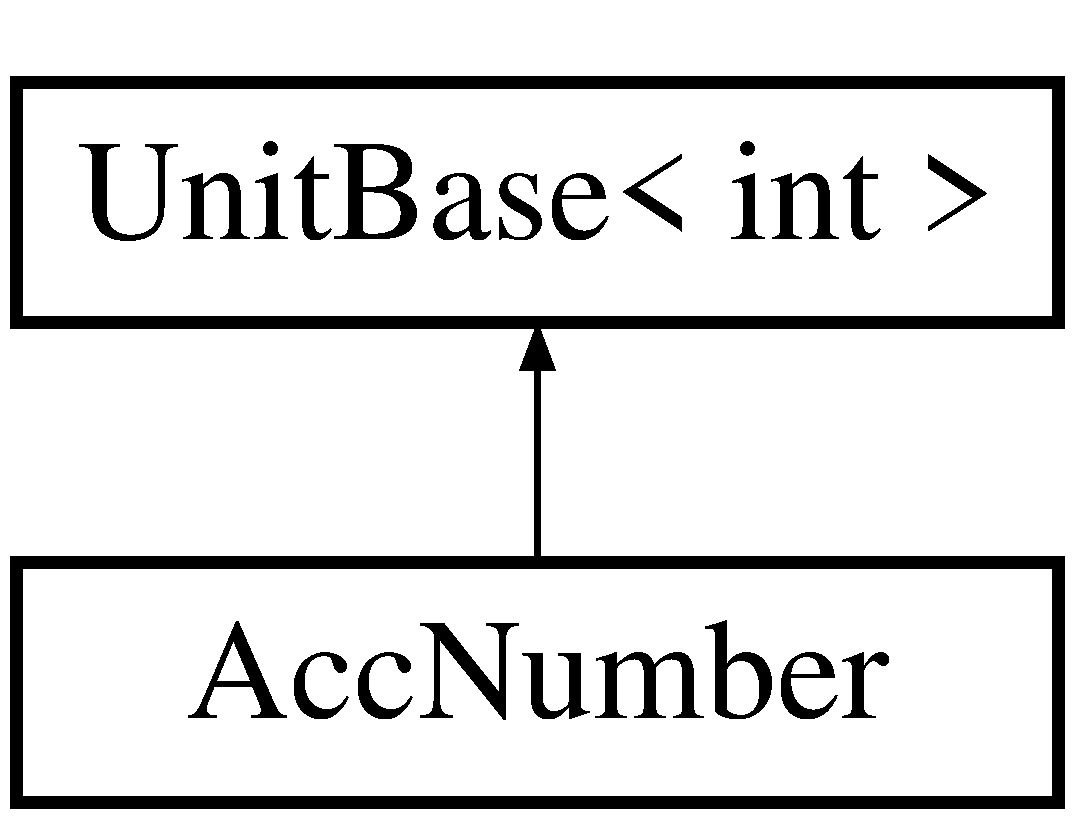
\includegraphics[height=2.000000cm]{classAccNumber}
\end{center}
\end{figure}
\subsection*{Public Member Functions}
\begin{DoxyCompactItemize}
\item 
\hypertarget{classAccNumber_a11a8a2ea0849a83365960758a5ff3362}{{\bfseries Acc\-Number} (int)  throw (invalid\-\_\-argument)}\label{classAccNumber_a11a8a2ea0849a83365960758a5ff3362}

\end{DoxyCompactItemize}
\subsection*{Additional Inherited Members}


\subsection{Detailed Description}
Define o número da conta de um Customer (Cliente). 

Este tipo básico tem a função de atribuir a cada conta um numero unico, identificando-\/a. 

The documentation for this class was generated from the following files\-:\begin{DoxyCompactItemize}
\item 
Base\-Unit.\-h\item 
Base\-Unit.\-cpp\end{DoxyCompactItemize}

\hypertarget{classAccount}{\section{Account Class Reference}
\label{d7/d10/classAccount}\index{Account@{Account}}
}


Conta; Onde ficarão armazenados os dados de conta de um cliente.  




{\ttfamily \#include $<$Entity\-Unit.\-h$>$}

\subsection*{Public Member Functions}
\begin{DoxyCompactItemize}
\item 
\hyperlink{classAccount_a94113be123fc89c3de8461cbb8251c83}{Account} (const \hyperlink{classAccNumber}{Acc\-Number} \&, const \hyperlink{classUsrType}{Acc\-Type} \&, const \hyperlink{classMoney}{Money} \&, const \hyperlink{classMoney}{Money} \&, const \hyperlink{classUsrId}{Usr\-Id} \&)
\begin{DoxyCompactList}\small\item\em Construtor base de \hyperlink{classAccount}{Account}. \end{DoxyCompactList}\item 
\hyperlink{classAccNumber}{Acc\-Number} \hyperlink{classAccount_a74f26f24e13e66a055bb8441dfb3d881}{get\-Acc\-Number} () const 
\begin{DoxyCompactList}\small\item\em Método que retorna o valor contido no atributo acc\-Number. \end{DoxyCompactList}\item 
void \hyperlink{classAccount_a3e669090168f13d2a8269af456546a1e}{set\-Acc\-Number} (const \hyperlink{classAccNumber}{Acc\-Number} \&)
\begin{DoxyCompactList}\small\item\em Método que define o valor do atributo acc\-Number. \end{DoxyCompactList}\item 
\hyperlink{classUsrType}{Acc\-Type} \hyperlink{classAccount_a34e1f7e507d7abdf575e4833d6f8d36b}{get\-Acc\-Type} () const 
\begin{DoxyCompactList}\small\item\em Método que retorna o valor contido no atributo acc\-Type. \end{DoxyCompactList}\item 
void \hyperlink{classAccount_a3a8e8aa0094b2af0496d45714f694256}{set\-Acc\-Type} (const \hyperlink{classUsrType}{Acc\-Type} \&)
\begin{DoxyCompactList}\small\item\em Método que define o valor do atributo acc\-Type. \end{DoxyCompactList}\item 
\hyperlink{classMoney}{Money} \hyperlink{classAccount_ac67a380f5f320a44f9bb464f6efd59f7}{get\-Limit} () const 
\begin{DoxyCompactList}\small\item\em Método que retorna o valor contido no atributo limit. \end{DoxyCompactList}\item 
void \hyperlink{classAccount_ada9bd7d0aee82d5b6c8f9831eb6fd8d5}{set\-Limit} (const \hyperlink{classMoney}{Money} \&)
\begin{DoxyCompactList}\small\item\em Método que define o valor do atributo limit. \end{DoxyCompactList}\item 
\hyperlink{classMoney}{Money} \hyperlink{classAccount_af9414bc748bf1923b2308544bbfd8b82}{get\-Balance} () const 
\begin{DoxyCompactList}\small\item\em Método que retorna o valor contido no atributo balance. \end{DoxyCompactList}\item 
void \hyperlink{classAccount_a0c54b27c54fd64b93d31aecdf7f3f302}{set\-Balance} (const \hyperlink{classMoney}{Money} \&)
\begin{DoxyCompactList}\small\item\em Método que define o valor do atributo balance. \end{DoxyCompactList}\item 
\hyperlink{classUsrId}{Usr\-Id} \hyperlink{classAccount_a59a83e5c5142f79402e79a8d42b36aed}{get\-Usr\-Id} () const 
\begin{DoxyCompactList}\small\item\em Método que retorna o valor contido no atributo usr\-Id. \end{DoxyCompactList}\item 
void \hyperlink{classAccount_a97146ede9747001294bcd41c74abd67a}{set\-Usr\-Id} (const \hyperlink{classUsrId}{Usr\-Id} \&)
\begin{DoxyCompactList}\small\item\em Método que define o valor do atributo usr\-Id. \end{DoxyCompactList}\end{DoxyCompactItemize}


\subsection{Detailed Description}
Conta; Onde ficarão armazenados os dados de conta de um cliente. 

Através de uma conta é possível acessar o módulo de Transações. 

\subsection{Constructor \& Destructor Documentation}
\hypertarget{classAccount_a94113be123fc89c3de8461cbb8251c83}{\index{Account@{Account}!Account@{Account}}
\index{Account@{Account}!Account@{Account}}
\subsubsection[{Account}]{\setlength{\rightskip}{0pt plus 5cm}Account\-::\-Account (
\begin{DoxyParamCaption}
\item[{const {\bf Acc\-Number} \&}]{acc\-Number, }
\item[{const {\bf Acc\-Type} \&}]{acc\-Type, }
\item[{const {\bf Money} \&}]{limit, }
\item[{const {\bf Money} \&}]{balance, }
\item[{const {\bf Usr\-Id} \&}]{usr\-Id}
\end{DoxyParamCaption}
)}}\label{d7/d10/classAccount_a94113be123fc89c3de8461cbb8251c83}


Construtor base de \hyperlink{classAccount}{Account}. 

Define os valores internos da classe automaticamente. 

\subsection{Member Function Documentation}
\hypertarget{classAccount_a74f26f24e13e66a055bb8441dfb3d881}{\index{Account@{Account}!get\-Acc\-Number@{get\-Acc\-Number}}
\index{get\-Acc\-Number@{get\-Acc\-Number}!Account@{Account}}
\subsubsection[{get\-Acc\-Number}]{\setlength{\rightskip}{0pt plus 5cm}{\bf Acc\-Number} Account\-::get\-Acc\-Number (
\begin{DoxyParamCaption}
{}
\end{DoxyParamCaption}
) const\hspace{0.3cm}{\ttfamily [inline]}}}\label{d7/d10/classAccount_a74f26f24e13e66a055bb8441dfb3d881}


Método que retorna o valor contido no atributo acc\-Number. 

O valor será retornado e o atributo não será modificado. \hypertarget{classAccount_a34e1f7e507d7abdf575e4833d6f8d36b}{\index{Account@{Account}!get\-Acc\-Type@{get\-Acc\-Type}}
\index{get\-Acc\-Type@{get\-Acc\-Type}!Account@{Account}}
\subsubsection[{get\-Acc\-Type}]{\setlength{\rightskip}{0pt plus 5cm}{\bf Acc\-Type} Account\-::get\-Acc\-Type (
\begin{DoxyParamCaption}
{}
\end{DoxyParamCaption}
) const\hspace{0.3cm}{\ttfamily [inline]}}}\label{d7/d10/classAccount_a34e1f7e507d7abdf575e4833d6f8d36b}


Método que retorna o valor contido no atributo acc\-Type. 

O valor será retornado e o atributo não será modificado. \hypertarget{classAccount_af9414bc748bf1923b2308544bbfd8b82}{\index{Account@{Account}!get\-Balance@{get\-Balance}}
\index{get\-Balance@{get\-Balance}!Account@{Account}}
\subsubsection[{get\-Balance}]{\setlength{\rightskip}{0pt plus 5cm}{\bf Money} Account\-::get\-Balance (
\begin{DoxyParamCaption}
{}
\end{DoxyParamCaption}
) const\hspace{0.3cm}{\ttfamily [inline]}}}\label{d7/d10/classAccount_af9414bc748bf1923b2308544bbfd8b82}


Método que retorna o valor contido no atributo balance. 

O valor será retornado e o atributo não será modificado. \hypertarget{classAccount_ac67a380f5f320a44f9bb464f6efd59f7}{\index{Account@{Account}!get\-Limit@{get\-Limit}}
\index{get\-Limit@{get\-Limit}!Account@{Account}}
\subsubsection[{get\-Limit}]{\setlength{\rightskip}{0pt plus 5cm}{\bf Money} Account\-::get\-Limit (
\begin{DoxyParamCaption}
{}
\end{DoxyParamCaption}
) const\hspace{0.3cm}{\ttfamily [inline]}}}\label{d7/d10/classAccount_ac67a380f5f320a44f9bb464f6efd59f7}


Método que retorna o valor contido no atributo limit. 

O valor será retornado e o atributo não será modificado. \hypertarget{classAccount_a59a83e5c5142f79402e79a8d42b36aed}{\index{Account@{Account}!get\-Usr\-Id@{get\-Usr\-Id}}
\index{get\-Usr\-Id@{get\-Usr\-Id}!Account@{Account}}
\subsubsection[{get\-Usr\-Id}]{\setlength{\rightskip}{0pt plus 5cm}{\bf Usr\-Id} Account\-::get\-Usr\-Id (
\begin{DoxyParamCaption}
{}
\end{DoxyParamCaption}
) const\hspace{0.3cm}{\ttfamily [inline]}}}\label{d7/d10/classAccount_a59a83e5c5142f79402e79a8d42b36aed}


Método que retorna o valor contido no atributo usr\-Id. 

O valor será retornado e o atributo não será modificado. \hypertarget{classAccount_a3e669090168f13d2a8269af456546a1e}{\index{Account@{Account}!set\-Acc\-Number@{set\-Acc\-Number}}
\index{set\-Acc\-Number@{set\-Acc\-Number}!Account@{Account}}
\subsubsection[{set\-Acc\-Number}]{\setlength{\rightskip}{0pt plus 5cm}void Account\-::set\-Acc\-Number (
\begin{DoxyParamCaption}
\item[{const {\bf Acc\-Number} \&}]{acc\-Number}
\end{DoxyParamCaption}
)}}\label{d7/d10/classAccount_a3e669090168f13d2a8269af456546a1e}


Método que define o valor do atributo acc\-Number. 

\hypertarget{classAccount_a3a8e8aa0094b2af0496d45714f694256}{\index{Account@{Account}!set\-Acc\-Type@{set\-Acc\-Type}}
\index{set\-Acc\-Type@{set\-Acc\-Type}!Account@{Account}}
\subsubsection[{set\-Acc\-Type}]{\setlength{\rightskip}{0pt plus 5cm}void Account\-::set\-Acc\-Type (
\begin{DoxyParamCaption}
\item[{const {\bf Acc\-Type} \&}]{acc\-Type}
\end{DoxyParamCaption}
)}}\label{d7/d10/classAccount_a3a8e8aa0094b2af0496d45714f694256}


Método que define o valor do atributo acc\-Type. 

\hypertarget{classAccount_a0c54b27c54fd64b93d31aecdf7f3f302}{\index{Account@{Account}!set\-Balance@{set\-Balance}}
\index{set\-Balance@{set\-Balance}!Account@{Account}}
\subsubsection[{set\-Balance}]{\setlength{\rightskip}{0pt plus 5cm}void Account\-::set\-Balance (
\begin{DoxyParamCaption}
\item[{const {\bf Money} \&}]{balance}
\end{DoxyParamCaption}
)}}\label{d7/d10/classAccount_a0c54b27c54fd64b93d31aecdf7f3f302}


Método que define o valor do atributo balance. 

\hypertarget{classAccount_ada9bd7d0aee82d5b6c8f9831eb6fd8d5}{\index{Account@{Account}!set\-Limit@{set\-Limit}}
\index{set\-Limit@{set\-Limit}!Account@{Account}}
\subsubsection[{set\-Limit}]{\setlength{\rightskip}{0pt plus 5cm}void Account\-::set\-Limit (
\begin{DoxyParamCaption}
\item[{const {\bf Money} \&}]{limit}
\end{DoxyParamCaption}
)}}\label{d7/d10/classAccount_ada9bd7d0aee82d5b6c8f9831eb6fd8d5}


Método que define o valor do atributo limit. 

\hypertarget{classAccount_a97146ede9747001294bcd41c74abd67a}{\index{Account@{Account}!set\-Usr\-Id@{set\-Usr\-Id}}
\index{set\-Usr\-Id@{set\-Usr\-Id}!Account@{Account}}
\subsubsection[{set\-Usr\-Id}]{\setlength{\rightskip}{0pt plus 5cm}void Account\-::set\-Usr\-Id (
\begin{DoxyParamCaption}
\item[{const {\bf Usr\-Id} \&}]{usr\-Id}
\end{DoxyParamCaption}
)}}\label{d7/d10/classAccount_a97146ede9747001294bcd41c74abd67a}


Método que define o valor do atributo usr\-Id. 



The documentation for this class was generated from the following files\-:\begin{DoxyCompactItemize}
\item 
Entity\-Unit.\-h\item 
Entity\-Unit.\-cpp\end{DoxyCompactItemize}

\hypertarget{classCtrlTransacAdm}{\subsection{Ctrl\-Transac\-Adm Class Reference}
\label{db/d25/classCtrlTransacAdm}\index{Ctrl\-Transac\-Adm@{Ctrl\-Transac\-Adm}}
}


Classe de negócio responsável pela administração de dados de pegamento e transações.  




{\ttfamily \#include $<$Transac\-Unit.\-h$>$}

Inheritance diagram for Ctrl\-Transac\-Adm\-:\begin{figure}[H]
\begin{center}
\leavevmode
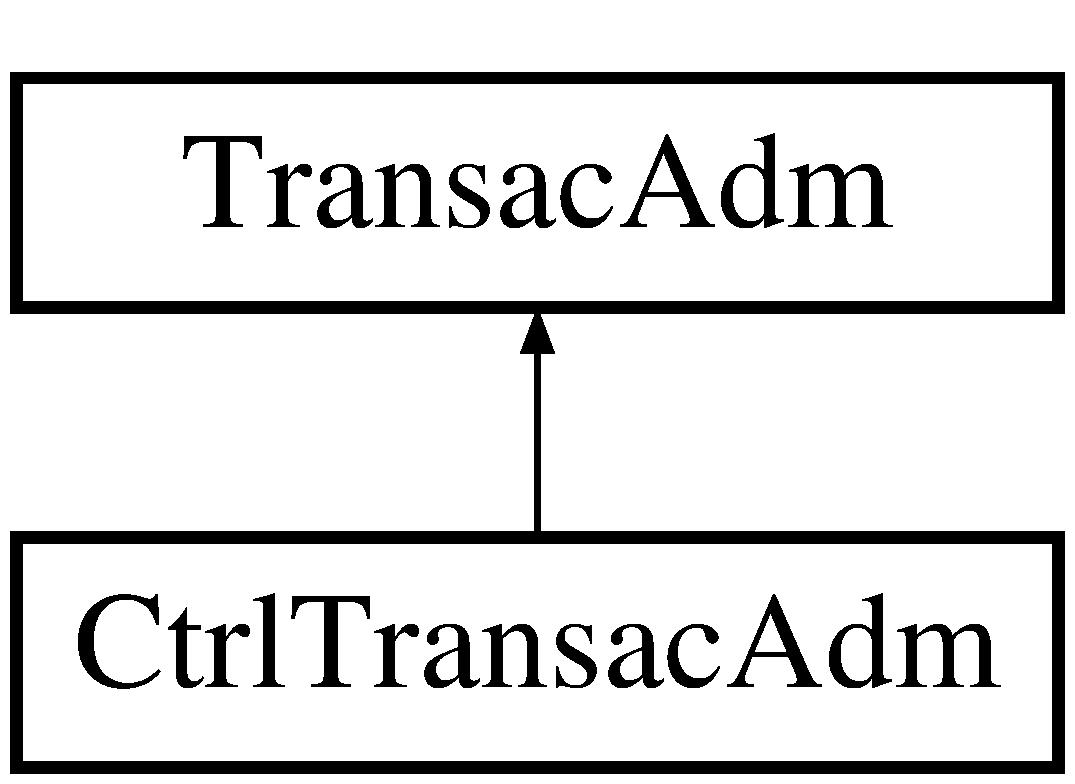
\includegraphics[height=2.000000cm]{db/d25/classCtrlTransacAdm}
\end{center}
\end{figure}
\subsubsection*{Public Member Functions}
\begin{DoxyCompactItemize}
\item 
void \hyperlink{classCtrlTransacAdm_a694267772d5ea46f715b8c3586d9b5fa}{withdraw} (\hyperlink{classAccNumber}{Acc\-Number}, \hyperlink{classMoney}{Money} $\ast$)  throw (invalid\-\_\-argument, Pers\-Error)
\begin{DoxyCompactList}\small\item\em Executa a retirada de dinheiro. \end{DoxyCompactList}\item 
void \hyperlink{classCtrlTransacAdm_a1e4a7b8ca4c50eb9a31371a28ffa00ff}{deposit} (\hyperlink{classAccNumber}{Acc\-Number}, \hyperlink{classMoney}{Money} $\ast$)  throw (invalid\-\_\-argument, Pers\-Error)
\begin{DoxyCompactList}\small\item\em Executa um depósito. \end{DoxyCompactList}\item 
\hyperlink{classPayCode}{Pay\-Code} $\ast$ \hyperlink{classCtrlTransacAdm_a1c10db63c827ee8071d7dc839154382a}{schedule\-Payment} (\hyperlink{classAccNumber}{Acc\-Number}, \hyperlink{classMoney}{Money} $\ast$, \hyperlink{classPayDay}{Pay\-Day} $\ast$)  throw (invalid\-\_\-argument, Pers\-Error)
\begin{DoxyCompactList}\small\item\em Agenda um pagamento. \end{DoxyCompactList}\item 
void \hyperlink{classCtrlTransacAdm_a3c2d1900a471725e5e5122de9fa30a35}{delete\-Payment} (\hyperlink{classPayCode}{Pay\-Code} $\ast$)  throw (invalid\-\_\-argument, Pers\-Error)
\begin{DoxyCompactList}\small\item\em Deleta um pagamento agendado. \end{DoxyCompactList}\item 
list$<$ \hyperlink{classPayment}{Payment} $>$ \hyperlink{classCtrlTransacAdm_aa7e00879d0ad01b7cd6b3ad61d4d8c65}{fetch\-Payment} (void)  throw (\-Pers\-Error)
\begin{DoxyCompactList}\small\item\em Recupera uma lista de todos os pagamentos registrados. \end{DoxyCompactList}\end{DoxyCompactItemize}


\subsubsection{Detailed Description}
Classe de negócio responsável pela administração de dados de pegamento e transações. 

Definition at line 34 of file Transac\-Unit.\-h.



\subsubsection{Member Function Documentation}
\hypertarget{classCtrlTransacAdm_a3c2d1900a471725e5e5122de9fa30a35}{\index{Ctrl\-Transac\-Adm@{Ctrl\-Transac\-Adm}!delete\-Payment@{delete\-Payment}}
\index{delete\-Payment@{delete\-Payment}!CtrlTransacAdm@{Ctrl\-Transac\-Adm}}
\paragraph[{delete\-Payment}]{\setlength{\rightskip}{0pt plus 5cm}void Ctrl\-Transac\-Adm\-::delete\-Payment (
\begin{DoxyParamCaption}
\item[{{\bf Pay\-Code} $\ast$}]{}
\end{DoxyParamCaption}
)  throw (invalid\-\_\-argument, {\bf Pers\-Error})\hspace{0.3cm}{\ttfamily [virtual]}}}\label{db/d25/classCtrlTransacAdm_a3c2d1900a471725e5e5122de9fa30a35}


Deleta um pagamento agendado. 



Implements \hyperlink{classTransacAdm_a76f27b0fc9e604695c4c601839d3b441}{Transac\-Adm}.



Definition at line 83 of file Transac\-Unit.\-cpp.

\hypertarget{classCtrlTransacAdm_a1e4a7b8ca4c50eb9a31371a28ffa00ff}{\index{Ctrl\-Transac\-Adm@{Ctrl\-Transac\-Adm}!deposit@{deposit}}
\index{deposit@{deposit}!CtrlTransacAdm@{Ctrl\-Transac\-Adm}}
\paragraph[{deposit}]{\setlength{\rightskip}{0pt plus 5cm}void Ctrl\-Transac\-Adm\-::deposit (
\begin{DoxyParamCaption}
\item[{{\bf Acc\-Number}}]{, }
\item[{{\bf Money} $\ast$}]{}
\end{DoxyParamCaption}
)  throw (invalid\-\_\-argument, {\bf Pers\-Error})\hspace{0.3cm}{\ttfamily [virtual]}}}\label{db/d25/classCtrlTransacAdm_a1e4a7b8ca4c50eb9a31371a28ffa00ff}


Executa um depósito. 



Implements \hyperlink{classTransacAdm_a9b6ffc8a521600094eb13510edcb33d7}{Transac\-Adm}.



Definition at line 31 of file Transac\-Unit.\-cpp.

\hypertarget{classCtrlTransacAdm_aa7e00879d0ad01b7cd6b3ad61d4d8c65}{\index{Ctrl\-Transac\-Adm@{Ctrl\-Transac\-Adm}!fetch\-Payment@{fetch\-Payment}}
\index{fetch\-Payment@{fetch\-Payment}!CtrlTransacAdm@{Ctrl\-Transac\-Adm}}
\paragraph[{fetch\-Payment}]{\setlength{\rightskip}{0pt plus 5cm}list$<$ {\bf Payment} $>$ Ctrl\-Transac\-Adm\-::fetch\-Payment (
\begin{DoxyParamCaption}
\item[{void}]{}
\end{DoxyParamCaption}
)  throw ({\bf Pers\-Error})\hspace{0.3cm}{\ttfamily [virtual]}}}\label{db/d25/classCtrlTransacAdm_aa7e00879d0ad01b7cd6b3ad61d4d8c65}


Recupera uma lista de todos os pagamentos registrados. 



Implements \hyperlink{classTransacAdm_ab3c02884c14540c1f520339581e88371}{Transac\-Adm}.



Definition at line 98 of file Transac\-Unit.\-cpp.

\hypertarget{classCtrlTransacAdm_a1c10db63c827ee8071d7dc839154382a}{\index{Ctrl\-Transac\-Adm@{Ctrl\-Transac\-Adm}!schedule\-Payment@{schedule\-Payment}}
\index{schedule\-Payment@{schedule\-Payment}!CtrlTransacAdm@{Ctrl\-Transac\-Adm}}
\paragraph[{schedule\-Payment}]{\setlength{\rightskip}{0pt plus 5cm}{\bf Pay\-Code} $\ast$ Ctrl\-Transac\-Adm\-::schedule\-Payment (
\begin{DoxyParamCaption}
\item[{{\bf Acc\-Number}}]{, }
\item[{{\bf Money} $\ast$}]{, }
\item[{{\bf Pay\-Day} $\ast$}]{}
\end{DoxyParamCaption}
)  throw (invalid\-\_\-argument, {\bf Pers\-Error})\hspace{0.3cm}{\ttfamily [virtual]}}}\label{db/d25/classCtrlTransacAdm_a1c10db63c827ee8071d7dc839154382a}


Agenda um pagamento. 



Implements \hyperlink{classTransacAdm_a6f350bc661f1a6460a31a0b02ccb8d3f}{Transac\-Adm}.



Definition at line 54 of file Transac\-Unit.\-cpp.

\hypertarget{classCtrlTransacAdm_a694267772d5ea46f715b8c3586d9b5fa}{\index{Ctrl\-Transac\-Adm@{Ctrl\-Transac\-Adm}!withdraw@{withdraw}}
\index{withdraw@{withdraw}!CtrlTransacAdm@{Ctrl\-Transac\-Adm}}
\paragraph[{withdraw}]{\setlength{\rightskip}{0pt plus 5cm}void Ctrl\-Transac\-Adm\-::withdraw (
\begin{DoxyParamCaption}
\item[{{\bf Acc\-Number}}]{, }
\item[{{\bf Money} $\ast$}]{}
\end{DoxyParamCaption}
)  throw (invalid\-\_\-argument, {\bf Pers\-Error})\hspace{0.3cm}{\ttfamily [virtual]}}}\label{db/d25/classCtrlTransacAdm_a694267772d5ea46f715b8c3586d9b5fa}


Executa a retirada de dinheiro. 



Implements \hyperlink{classTransacAdm_a128750caeeec2cd48a4a01e6ce9f701c}{Transac\-Adm}.



Definition at line 3 of file Transac\-Unit.\-cpp.



The documentation for this class was generated from the following files\-:\begin{DoxyCompactItemize}
\item 
Transac\-Unit.\-h\item 
Transac\-Unit.\-cpp\end{DoxyCompactItemize}

\hypertarget{classCtrlUserAccAdm}{\subsection{Ctrl\-User\-Acc\-Adm Class Reference}
\label{db/d93/classCtrlUserAccAdm}\index{Ctrl\-User\-Acc\-Adm@{Ctrl\-User\-Acc\-Adm}}
}


Classe de negócio responsável pela administração de dados de contas.  




{\ttfamily \#include $<$User\-Unit.\-h$>$}

Inheritance diagram for Ctrl\-User\-Acc\-Adm\-:\begin{figure}[H]
\begin{center}
\leavevmode
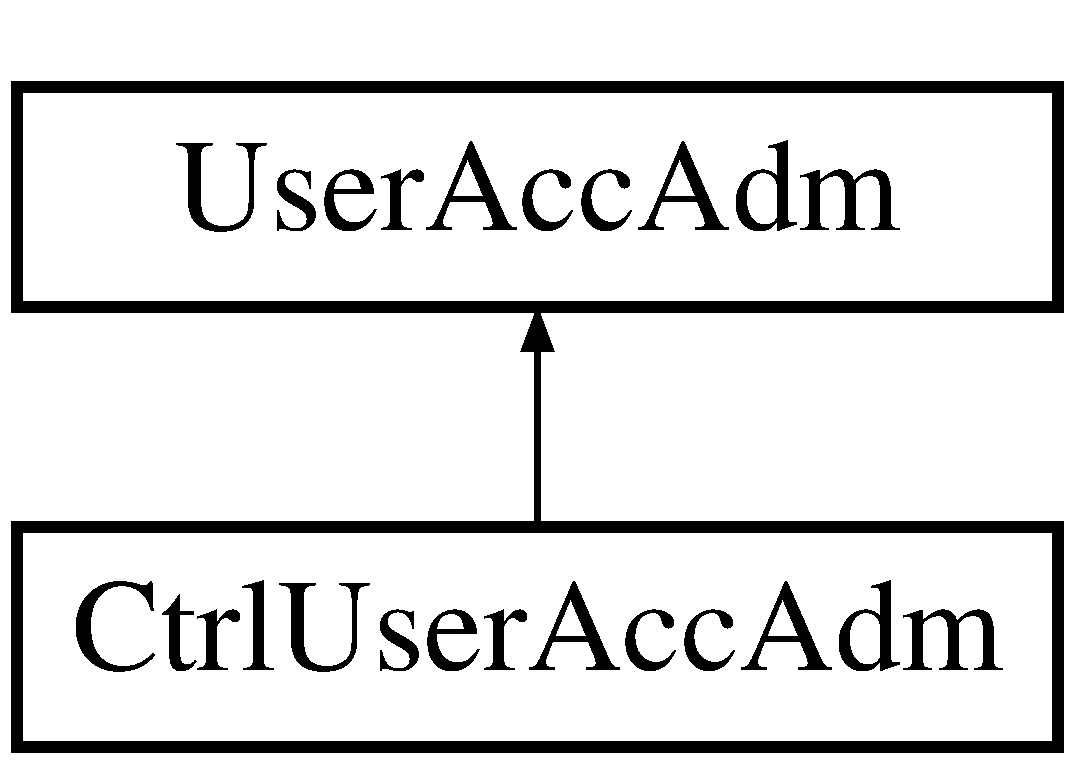
\includegraphics[height=2.000000cm]{db/d93/classCtrlUserAccAdm}
\end{center}
\end{figure}
\subsubsection*{Public Member Functions}
\begin{DoxyCompactItemize}
\item 
void \hyperlink{classCtrlUserAccAdm_aa08ff58074dc0cb37c4d878e04b34adc}{create\-Account} (\hyperlink{classUsrType}{Acc\-Type} $\ast$, \hyperlink{classMoney}{Money} $\ast$, \hyperlink{classMoney}{Money} $\ast$, \hyperlink{classUsrId}{Usr\-Id})  throw (\-Pers\-Error)
\begin{DoxyCompactList}\small\item\em Cria uma conta. \end{DoxyCompactList}\item 
void \hyperlink{classCtrlUserAccAdm_aff45f0827b96208a4ccd6ae22610c5e3}{delete\-Account} (\hyperlink{classAccNumber}{Acc\-Number} $\ast$)  throw (invalid\-\_\-argument, Pers\-Error)
\begin{DoxyCompactList}\small\item\em Deleta uma conta. \end{DoxyCompactList}\item 
void \hyperlink{classCtrlUserAccAdm_a31433e164de26c03becbc04f57c029ea}{block\-Account} (\hyperlink{classAccNumber}{Acc\-Number} $\ast$)  throw (invalid\-\_\-argument, Pers\-Error)
\begin{DoxyCompactList}\small\item\em Bloqueia uma conta. \end{DoxyCompactList}\item 
void \hyperlink{classCtrlUserAccAdm_ad129cb69fc2a73cfb40bd52063d4369e}{unblock\-Account} (\hyperlink{classAccNumber}{Acc\-Number} $\ast$)  throw (invalid\-\_\-argument, Pers\-Error)
\begin{DoxyCompactList}\small\item\em Desbloqueia uma conta. \end{DoxyCompactList}\item 
list$<$ \hyperlink{classAccount}{Account} $>$ \hyperlink{classCtrlUserAccAdm_a42e34f0780b86f393c25010e693450c2}{fetch\-Account} (void)  throw (\-Pers\-Error)
\begin{DoxyCompactList}\small\item\em Recupera uma lista com todas as contas registradas. \end{DoxyCompactList}\item 
\hyperlink{classAccount}{Account} \hyperlink{classCtrlUserAccAdm_a94e2637bedec766614095eee44bc9f38}{fetch\-Account} (\hyperlink{classAccNumber}{Acc\-Number})  throw (\-Pers\-Error)
\begin{DoxyCompactList}\small\item\em Recupera os dados da conta de uma conta em específico. \end{DoxyCompactList}\item 
void \hyperlink{classCtrlUserAccAdm_a76260af4ccd5301504a50adbead90129}{edit\-Acc\-Type} (\hyperlink{classAccNumber}{Acc\-Number} $\ast$, \hyperlink{classUsrType}{Acc\-Type} $\ast$)  throw (invalid\-\_\-argument, Pers\-Error)
\begin{DoxyCompactList}\small\item\em Edita o tipo de um conta. \end{DoxyCompactList}\item 
void \hyperlink{classCtrlUserAccAdm_a91d3db6c6233065aff60cbc679116467}{edit\-Acc\-Limit} (\hyperlink{classAccNumber}{Acc\-Number} $\ast$, \hyperlink{classMoney}{Money} $\ast$)  throw (invalid\-\_\-argument, Pers\-Error)
\begin{DoxyCompactList}\small\item\em Edita o Limite de uma conta. \end{DoxyCompactList}\end{DoxyCompactItemize}


\subsubsection{Detailed Description}
Classe de negócio responsável pela administração de dados de contas. 

Definition at line 62 of file User\-Unit.\-h.



\subsubsection{Member Function Documentation}
\hypertarget{classCtrlUserAccAdm_a31433e164de26c03becbc04f57c029ea}{\index{Ctrl\-User\-Acc\-Adm@{Ctrl\-User\-Acc\-Adm}!block\-Account@{block\-Account}}
\index{block\-Account@{block\-Account}!CtrlUserAccAdm@{Ctrl\-User\-Acc\-Adm}}
\paragraph[{block\-Account}]{\setlength{\rightskip}{0pt plus 5cm}void Ctrl\-User\-Acc\-Adm\-::block\-Account (
\begin{DoxyParamCaption}
\item[{{\bf Acc\-Number} $\ast$}]{}
\end{DoxyParamCaption}
)  throw (invalid\-\_\-argument, {\bf Pers\-Error})\hspace{0.3cm}{\ttfamily [virtual]}}}\label{db/d93/classCtrlUserAccAdm_a31433e164de26c03becbc04f57c029ea}


Bloqueia uma conta. 



Implements \hyperlink{classUserAccAdm_ad9cdd01395ad7dd1b2c0887fe12b71b8}{User\-Acc\-Adm}.



Definition at line 100 of file User\-Unit.\-cpp.

\hypertarget{classCtrlUserAccAdm_aa08ff58074dc0cb37c4d878e04b34adc}{\index{Ctrl\-User\-Acc\-Adm@{Ctrl\-User\-Acc\-Adm}!create\-Account@{create\-Account}}
\index{create\-Account@{create\-Account}!CtrlUserAccAdm@{Ctrl\-User\-Acc\-Adm}}
\paragraph[{create\-Account}]{\setlength{\rightskip}{0pt plus 5cm}void Ctrl\-User\-Acc\-Adm\-::create\-Account (
\begin{DoxyParamCaption}
\item[{{\bf Acc\-Type} $\ast$}]{, }
\item[{{\bf Money} $\ast$}]{, }
\item[{{\bf Money} $\ast$}]{, }
\item[{{\bf Usr\-Id}}]{}
\end{DoxyParamCaption}
)  throw ({\bf Pers\-Error})\hspace{0.3cm}{\ttfamily [virtual]}}}\label{db/d93/classCtrlUserAccAdm_aa08ff58074dc0cb37c4d878e04b34adc}


Cria uma conta. 



Implements \hyperlink{classUserAccAdm_a8bf3fc2dc45a1f13dbd8388cc37a26a2}{User\-Acc\-Adm}.



Definition at line 70 of file User\-Unit.\-cpp.

\hypertarget{classCtrlUserAccAdm_aff45f0827b96208a4ccd6ae22610c5e3}{\index{Ctrl\-User\-Acc\-Adm@{Ctrl\-User\-Acc\-Adm}!delete\-Account@{delete\-Account}}
\index{delete\-Account@{delete\-Account}!CtrlUserAccAdm@{Ctrl\-User\-Acc\-Adm}}
\paragraph[{delete\-Account}]{\setlength{\rightskip}{0pt plus 5cm}void Ctrl\-User\-Acc\-Adm\-::delete\-Account (
\begin{DoxyParamCaption}
\item[{{\bf Acc\-Number} $\ast$}]{}
\end{DoxyParamCaption}
)  throw (invalid\-\_\-argument, {\bf Pers\-Error})\hspace{0.3cm}{\ttfamily [virtual]}}}\label{db/d93/classCtrlUserAccAdm_aff45f0827b96208a4ccd6ae22610c5e3}


Deleta uma conta. 



Implements \hyperlink{classUserAccAdm_a8257788e5e7d125b7482e490a6d71550}{User\-Acc\-Adm}.



Definition at line 87 of file User\-Unit.\-cpp.

\hypertarget{classCtrlUserAccAdm_a91d3db6c6233065aff60cbc679116467}{\index{Ctrl\-User\-Acc\-Adm@{Ctrl\-User\-Acc\-Adm}!edit\-Acc\-Limit@{edit\-Acc\-Limit}}
\index{edit\-Acc\-Limit@{edit\-Acc\-Limit}!CtrlUserAccAdm@{Ctrl\-User\-Acc\-Adm}}
\paragraph[{edit\-Acc\-Limit}]{\setlength{\rightskip}{0pt plus 5cm}void Ctrl\-User\-Acc\-Adm\-::edit\-Acc\-Limit (
\begin{DoxyParamCaption}
\item[{{\bf Acc\-Number} $\ast$}]{, }
\item[{{\bf Money} $\ast$}]{}
\end{DoxyParamCaption}
)  throw (invalid\-\_\-argument, {\bf Pers\-Error})\hspace{0.3cm}{\ttfamily [virtual]}}}\label{db/d93/classCtrlUserAccAdm_a91d3db6c6233065aff60cbc679116467}


Edita o Limite de uma conta. 



Implements \hyperlink{classUserAccAdm_a43f0bb580d63a9c782e8c83417562a17}{User\-Acc\-Adm}.



Definition at line 157 of file User\-Unit.\-cpp.

\hypertarget{classCtrlUserAccAdm_a76260af4ccd5301504a50adbead90129}{\index{Ctrl\-User\-Acc\-Adm@{Ctrl\-User\-Acc\-Adm}!edit\-Acc\-Type@{edit\-Acc\-Type}}
\index{edit\-Acc\-Type@{edit\-Acc\-Type}!CtrlUserAccAdm@{Ctrl\-User\-Acc\-Adm}}
\paragraph[{edit\-Acc\-Type}]{\setlength{\rightskip}{0pt plus 5cm}void Ctrl\-User\-Acc\-Adm\-::edit\-Acc\-Type (
\begin{DoxyParamCaption}
\item[{{\bf Acc\-Number} $\ast$}]{, }
\item[{{\bf Acc\-Type} $\ast$}]{}
\end{DoxyParamCaption}
)  throw (invalid\-\_\-argument, {\bf Pers\-Error})\hspace{0.3cm}{\ttfamily [virtual]}}}\label{db/d93/classCtrlUserAccAdm_a76260af4ccd5301504a50adbead90129}


Edita o tipo de um conta. 



Implements \hyperlink{classUserAccAdm_a80d61347b448e3ae9bdca4e02e65bcd1}{User\-Acc\-Adm}.



Definition at line 144 of file User\-Unit.\-cpp.

\hypertarget{classCtrlUserAccAdm_a42e34f0780b86f393c25010e693450c2}{\index{Ctrl\-User\-Acc\-Adm@{Ctrl\-User\-Acc\-Adm}!fetch\-Account@{fetch\-Account}}
\index{fetch\-Account@{fetch\-Account}!CtrlUserAccAdm@{Ctrl\-User\-Acc\-Adm}}
\paragraph[{fetch\-Account}]{\setlength{\rightskip}{0pt plus 5cm}list$<$ {\bf Account} $>$ Ctrl\-User\-Acc\-Adm\-::fetch\-Account (
\begin{DoxyParamCaption}
\item[{void}]{}
\end{DoxyParamCaption}
)  throw ({\bf Pers\-Error})\hspace{0.3cm}{\ttfamily [virtual]}}}\label{db/d93/classCtrlUserAccAdm_a42e34f0780b86f393c25010e693450c2}


Recupera uma lista com todas as contas registradas. 



Implements \hyperlink{classUserAccAdm_aa84b9df92ad9e11b1d9c71e9350efdc7}{User\-Acc\-Adm}.



Definition at line 113 of file User\-Unit.\-cpp.

\hypertarget{classCtrlUserAccAdm_a94e2637bedec766614095eee44bc9f38}{\index{Ctrl\-User\-Acc\-Adm@{Ctrl\-User\-Acc\-Adm}!fetch\-Account@{fetch\-Account}}
\index{fetch\-Account@{fetch\-Account}!CtrlUserAccAdm@{Ctrl\-User\-Acc\-Adm}}
\paragraph[{fetch\-Account}]{\setlength{\rightskip}{0pt plus 5cm}{\bf Account} Ctrl\-User\-Acc\-Adm\-::fetch\-Account (
\begin{DoxyParamCaption}
\item[{{\bf Acc\-Number}}]{}
\end{DoxyParamCaption}
)  throw ({\bf Pers\-Error})\hspace{0.3cm}{\ttfamily [virtual]}}}\label{db/d93/classCtrlUserAccAdm_a94e2637bedec766614095eee44bc9f38}


Recupera os dados da conta de uma conta em específico. 



Implements \hyperlink{classUserAccAdm_a5957dcbf58d30b171a6ca0967dacf2d9}{User\-Acc\-Adm}.



Definition at line 122 of file User\-Unit.\-cpp.

\hypertarget{classCtrlUserAccAdm_ad129cb69fc2a73cfb40bd52063d4369e}{\index{Ctrl\-User\-Acc\-Adm@{Ctrl\-User\-Acc\-Adm}!unblock\-Account@{unblock\-Account}}
\index{unblock\-Account@{unblock\-Account}!CtrlUserAccAdm@{Ctrl\-User\-Acc\-Adm}}
\paragraph[{unblock\-Account}]{\setlength{\rightskip}{0pt plus 5cm}void Ctrl\-User\-Acc\-Adm\-::unblock\-Account (
\begin{DoxyParamCaption}
\item[{{\bf Acc\-Number} $\ast$}]{}
\end{DoxyParamCaption}
)  throw (invalid\-\_\-argument, {\bf Pers\-Error})\hspace{0.3cm}{\ttfamily [virtual]}}}\label{db/d93/classCtrlUserAccAdm_ad129cb69fc2a73cfb40bd52063d4369e}


Desbloqueia uma conta. 



Implements \hyperlink{classUserAccAdm_ae179b3e21f336b325452eb3c0981b0d9}{User\-Acc\-Adm}.



Definition at line 131 of file User\-Unit.\-cpp.



The documentation for this class was generated from the following files\-:\begin{DoxyCompactItemize}
\item 
User\-Unit.\-h\item 
User\-Unit.\-cpp\end{DoxyCompactItemize}

\hypertarget{classCtrlUserCusAdm}{\subsection{Ctrl\-User\-Cus\-Adm Class Reference}
\label{d8/d93/classCtrlUserCusAdm}\index{Ctrl\-User\-Cus\-Adm@{Ctrl\-User\-Cus\-Adm}}
}


Classe de negócio responsável por administrar dados de clientes.  




{\ttfamily \#include $<$User\-Unit.\-h$>$}

Inheritance diagram for Ctrl\-User\-Cus\-Adm\-:\begin{figure}[H]
\begin{center}
\leavevmode
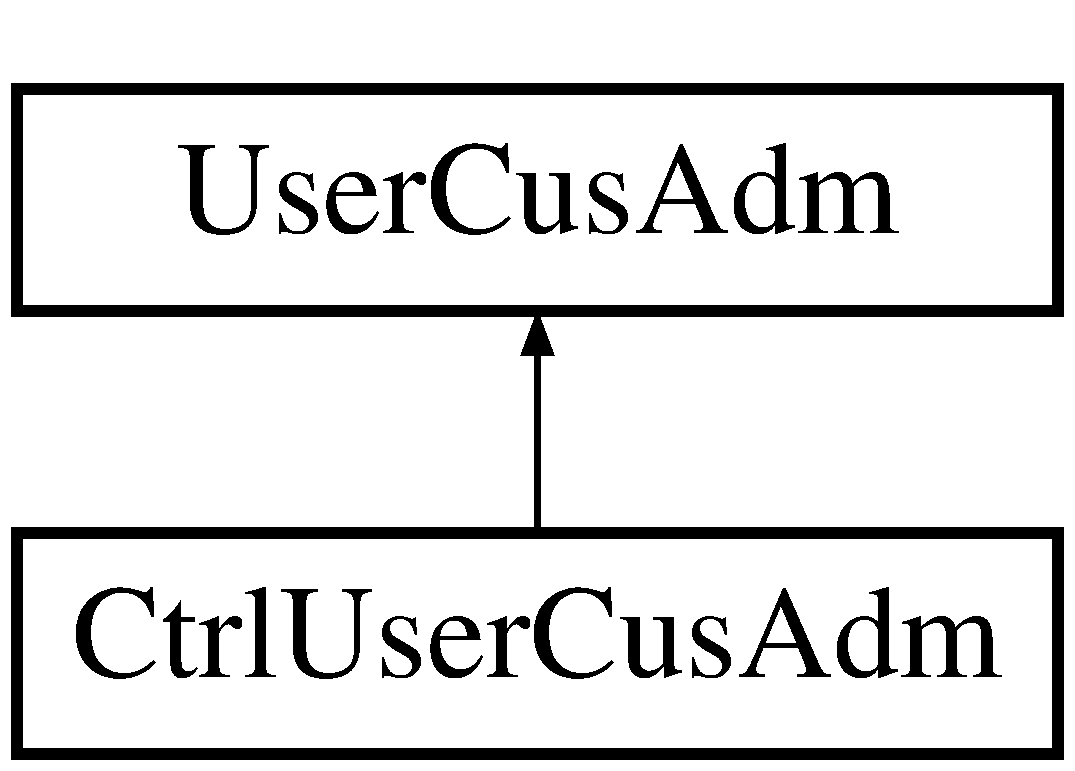
\includegraphics[height=2.000000cm]{d8/d93/classCtrlUserCusAdm}
\end{center}
\end{figure}
\subsubsection*{Public Member Functions}
\begin{DoxyCompactItemize}
\item 
void \hyperlink{classCtrlUserCusAdm_a824dda2b1f70cb6c855b0f0741cf1ae3}{change\-Password} (\hyperlink{classUsrId}{Usr\-Id}, \hyperlink{classUsrPassword}{Usr\-Password} $\ast$)  throw (\-Pers\-Error)
\begin{DoxyCompactList}\small\item\em Modifica a senha do cliente. \end{DoxyCompactList}\item 
\hyperlink{classUsrId}{Usr\-Id} \hyperlink{classCtrlUserCusAdm_acaef9cd1fb9a32deff009e1ddc2c7a5f}{create\-Customer} (\hyperlink{classUsrName}{Usr\-Name} $\ast$, \hyperlink{classUsrPassword}{Usr\-Password} $\ast$)  throw (invalid\-\_\-argument, Pers\-Error)
\begin{DoxyCompactList}\small\item\em Cria um cliente. \end{DoxyCompactList}\item 
void \hyperlink{classCtrlUserCusAdm_a4155af77de74ea82bcd54cd2ac23daed}{edit\-Cus\-Name} (\hyperlink{classUsrId}{Usr\-Id} $\ast$, \hyperlink{classUsrName}{Usr\-Name} $\ast$)  throw (invalid\-\_\-argument, Pers\-Error)
\begin{DoxyCompactList}\small\item\em Edita o nome do cliente. \end{DoxyCompactList}\item 
\hyperlink{classCustomer}{Customer} \hyperlink{classCtrlUserCusAdm_a63722fe2ad890dfbafc6bf8104ab51f2}{fetch\-Customer} (\hyperlink{classUsrId}{Usr\-Id})  throw (\-Pers\-Error)
\begin{DoxyCompactList}\small\item\em Recupera so dados do cliente. \end{DoxyCompactList}\end{DoxyCompactItemize}


\subsubsection{Detailed Description}
Classe de negócio responsável por administrar dados de clientes. 

Definition at line 159 of file User\-Unit.\-h.



\subsubsection{Member Function Documentation}
\hypertarget{classCtrlUserCusAdm_a824dda2b1f70cb6c855b0f0741cf1ae3}{\index{Ctrl\-User\-Cus\-Adm@{Ctrl\-User\-Cus\-Adm}!change\-Password@{change\-Password}}
\index{change\-Password@{change\-Password}!CtrlUserCusAdm@{Ctrl\-User\-Cus\-Adm}}
\paragraph[{change\-Password}]{\setlength{\rightskip}{0pt plus 5cm}void Ctrl\-User\-Cus\-Adm\-::change\-Password (
\begin{DoxyParamCaption}
\item[{{\bf Usr\-Id}}]{, }
\item[{{\bf Usr\-Password} $\ast$}]{}
\end{DoxyParamCaption}
)  throw ({\bf Pers\-Error})\hspace{0.3cm}{\ttfamily [virtual]}}}\label{d8/d93/classCtrlUserCusAdm_a824dda2b1f70cb6c855b0f0741cf1ae3}


Modifica a senha do cliente. 



Implements \hyperlink{classUserCusAdm_aed6d785e91a48c205df8c64736dbf3cf}{User\-Cus\-Adm}.



Definition at line 403 of file User\-Unit.\-cpp.

\hypertarget{classCtrlUserCusAdm_acaef9cd1fb9a32deff009e1ddc2c7a5f}{\index{Ctrl\-User\-Cus\-Adm@{Ctrl\-User\-Cus\-Adm}!create\-Customer@{create\-Customer}}
\index{create\-Customer@{create\-Customer}!CtrlUserCusAdm@{Ctrl\-User\-Cus\-Adm}}
\paragraph[{create\-Customer}]{\setlength{\rightskip}{0pt plus 5cm}{\bf Usr\-Id} Ctrl\-User\-Cus\-Adm\-::create\-Customer (
\begin{DoxyParamCaption}
\item[{{\bf Usr\-Name} $\ast$}]{, }
\item[{{\bf Usr\-Password} $\ast$}]{}
\end{DoxyParamCaption}
)  throw (invalid\-\_\-argument, {\bf Pers\-Error})\hspace{0.3cm}{\ttfamily [virtual]}}}\label{d8/d93/classCtrlUserCusAdm_acaef9cd1fb9a32deff009e1ddc2c7a5f}


Cria um cliente. 



Implements \hyperlink{classUserCusAdm_a4775bb30caf44192349db204b95b2b2f}{User\-Cus\-Adm}.



Definition at line 410 of file User\-Unit.\-cpp.

\hypertarget{classCtrlUserCusAdm_a4155af77de74ea82bcd54cd2ac23daed}{\index{Ctrl\-User\-Cus\-Adm@{Ctrl\-User\-Cus\-Adm}!edit\-Cus\-Name@{edit\-Cus\-Name}}
\index{edit\-Cus\-Name@{edit\-Cus\-Name}!CtrlUserCusAdm@{Ctrl\-User\-Cus\-Adm}}
\paragraph[{edit\-Cus\-Name}]{\setlength{\rightskip}{0pt plus 5cm}void Ctrl\-User\-Cus\-Adm\-::edit\-Cus\-Name (
\begin{DoxyParamCaption}
\item[{{\bf Usr\-Id} $\ast$}]{, }
\item[{{\bf Usr\-Name} $\ast$}]{}
\end{DoxyParamCaption}
)  throw (invalid\-\_\-argument, {\bf Pers\-Error})\hspace{0.3cm}{\ttfamily [virtual]}}}\label{d8/d93/classCtrlUserCusAdm_a4155af77de74ea82bcd54cd2ac23daed}


Edita o nome do cliente. 



Implements \hyperlink{classUserCusAdm_a2fffe3697904fb67ca285261276e1252}{User\-Cus\-Adm}.



Definition at line 435 of file User\-Unit.\-cpp.

\hypertarget{classCtrlUserCusAdm_a63722fe2ad890dfbafc6bf8104ab51f2}{\index{Ctrl\-User\-Cus\-Adm@{Ctrl\-User\-Cus\-Adm}!fetch\-Customer@{fetch\-Customer}}
\index{fetch\-Customer@{fetch\-Customer}!CtrlUserCusAdm@{Ctrl\-User\-Cus\-Adm}}
\paragraph[{fetch\-Customer}]{\setlength{\rightskip}{0pt plus 5cm}{\bf Customer} Ctrl\-User\-Cus\-Adm\-::fetch\-Customer (
\begin{DoxyParamCaption}
\item[{{\bf Usr\-Id}}]{}
\end{DoxyParamCaption}
)  throw ({\bf Pers\-Error})\hspace{0.3cm}{\ttfamily [virtual]}}}\label{d8/d93/classCtrlUserCusAdm_a63722fe2ad890dfbafc6bf8104ab51f2}


Recupera so dados do cliente. 



Implements \hyperlink{classUserCusAdm_a8a67bf25c965e931be912f33449e0f8a}{User\-Cus\-Adm}.



Definition at line 447 of file User\-Unit.\-cpp.



The documentation for this class was generated from the following files\-:\begin{DoxyCompactItemize}
\item 
User\-Unit.\-h\item 
User\-Unit.\-cpp\end{DoxyCompactItemize}

\hypertarget{classCtrlUserLogin}{\subsection{Ctrl\-User\-Login Class Reference}
\label{d0/d43/classCtrlUserLogin}\index{Ctrl\-User\-Login@{Ctrl\-User\-Login}}
}


Classe de negócio responsável por controlar os dados de login.  




{\ttfamily \#include $<$User\-Unit.\-h$>$}

Inheritance diagram for Ctrl\-User\-Login\-:\begin{figure}[H]
\begin{center}
\leavevmode
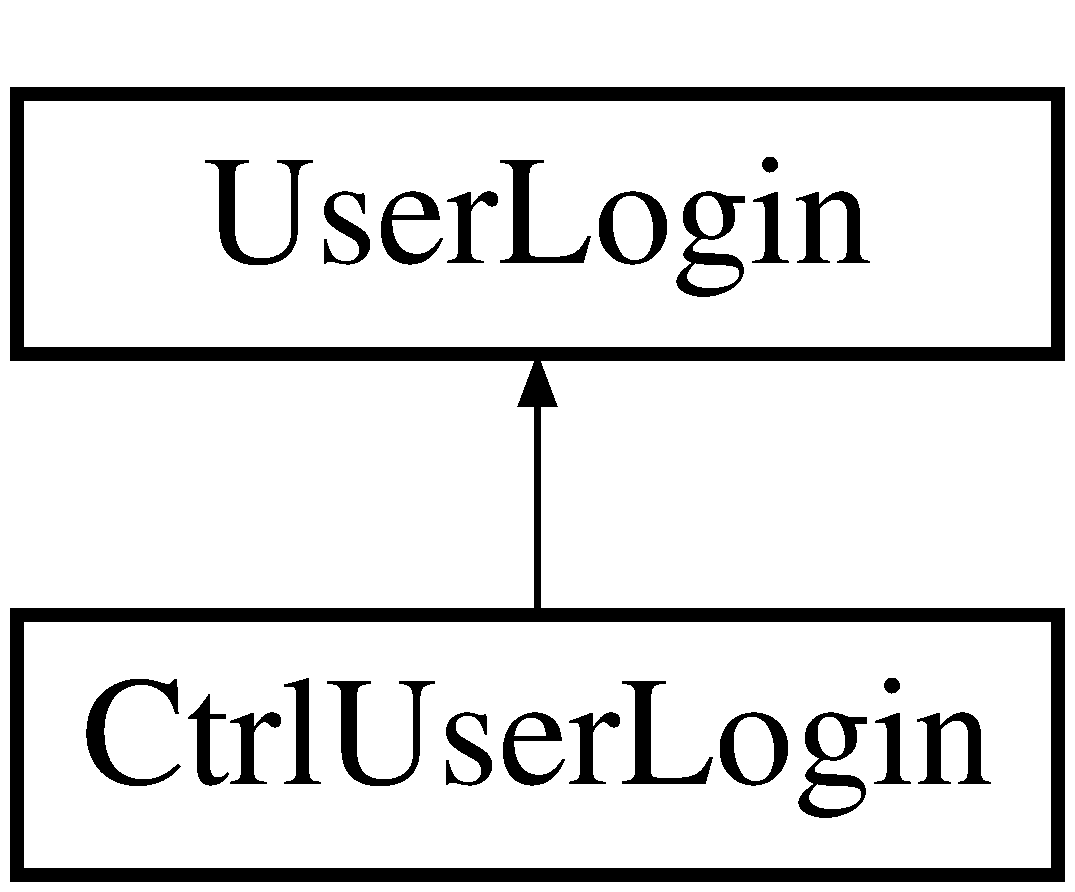
\includegraphics[height=2.000000cm]{d0/d43/classCtrlUserLogin}
\end{center}
\end{figure}
\subsubsection*{Public Member Functions}
\begin{DoxyCompactItemize}
\item 
\hyperlink{classUsrType}{Man\-Type} \hyperlink{classCtrlUserLogin_a023e4356e844e4824158ece586dbb07f}{autent} (\hyperlink{classUsrMatric}{Usr\-Matric} $\ast$, \hyperlink{classUsrPassword}{Usr\-Password} $\ast$)  throw (invalid\-\_\-argument, Pers\-Error)
\begin{DoxyCompactList}\small\item\em Autentica um administrador / gerente. \end{DoxyCompactList}\item 
void \hyperlink{classCtrlUserLogin_ae590a9174f5519037f92a7de7a2f9784}{autent} (\hyperlink{classAccNumber}{Acc\-Number} $\ast$, \hyperlink{classUsrPassword}{Usr\-Password} $\ast$)  throw (invalid\-\_\-argument, Pers\-Error)
\begin{DoxyCompactList}\small\item\em Autentica um cliente. \end{DoxyCompactList}\end{DoxyCompactItemize}


\subsubsection{Detailed Description}
Classe de negócio responsável por controlar os dados de login. 

Definition at line 21 of file User\-Unit.\-h.



\subsubsection{Member Function Documentation}
\hypertarget{classCtrlUserLogin_a023e4356e844e4824158ece586dbb07f}{\index{Ctrl\-User\-Login@{Ctrl\-User\-Login}!autent@{autent}}
\index{autent@{autent}!CtrlUserLogin@{Ctrl\-User\-Login}}
\paragraph[{autent}]{\setlength{\rightskip}{0pt plus 5cm}{\bf Man\-Type} Ctrl\-User\-Login\-::autent (
\begin{DoxyParamCaption}
\item[{{\bf Usr\-Matric} $\ast$}]{, }
\item[{{\bf Usr\-Password} $\ast$}]{}
\end{DoxyParamCaption}
)  throw (invalid\-\_\-argument, {\bf Pers\-Error})\hspace{0.3cm}{\ttfamily [virtual]}}}\label{d0/d43/classCtrlUserLogin_a023e4356e844e4824158ece586dbb07f}


Autentica um administrador / gerente. 



Implements \hyperlink{classUserLogin_a15141f463faedae30e40115658fcc0b9}{User\-Login}.



Definition at line 9 of file User\-Unit.\-cpp.

\hypertarget{classCtrlUserLogin_ae590a9174f5519037f92a7de7a2f9784}{\index{Ctrl\-User\-Login@{Ctrl\-User\-Login}!autent@{autent}}
\index{autent@{autent}!CtrlUserLogin@{Ctrl\-User\-Login}}
\paragraph[{autent}]{\setlength{\rightskip}{0pt plus 5cm}void Ctrl\-User\-Login\-::autent (
\begin{DoxyParamCaption}
\item[{{\bf Acc\-Number} $\ast$}]{, }
\item[{{\bf Usr\-Password} $\ast$}]{}
\end{DoxyParamCaption}
)  throw (invalid\-\_\-argument, {\bf Pers\-Error})\hspace{0.3cm}{\ttfamily [virtual]}}}\label{d0/d43/classCtrlUserLogin_ae590a9174f5519037f92a7de7a2f9784}


Autentica um cliente. 



Implements \hyperlink{classUserLogin_a7163b2b97915fd0e3e5d3f76c2af44da}{User\-Login}.



Definition at line 22 of file User\-Unit.\-cpp.



The documentation for this class was generated from the following files\-:\begin{DoxyCompactItemize}
\item 
User\-Unit.\-h\item 
User\-Unit.\-cpp\end{DoxyCompactItemize}

\hypertarget{classCtrlUserManAdm}{\subsection{Ctrl\-User\-Man\-Adm Class Reference}
\label{d4/d17/classCtrlUserManAdm}\index{Ctrl\-User\-Man\-Adm@{Ctrl\-User\-Man\-Adm}}
}


Classe de negócio para administração de dados de Gerentes e Administradores.  




{\ttfamily \#include $<$User\-Unit.\-h$>$}

Inheritance diagram for Ctrl\-User\-Man\-Adm\-:\begin{figure}[H]
\begin{center}
\leavevmode
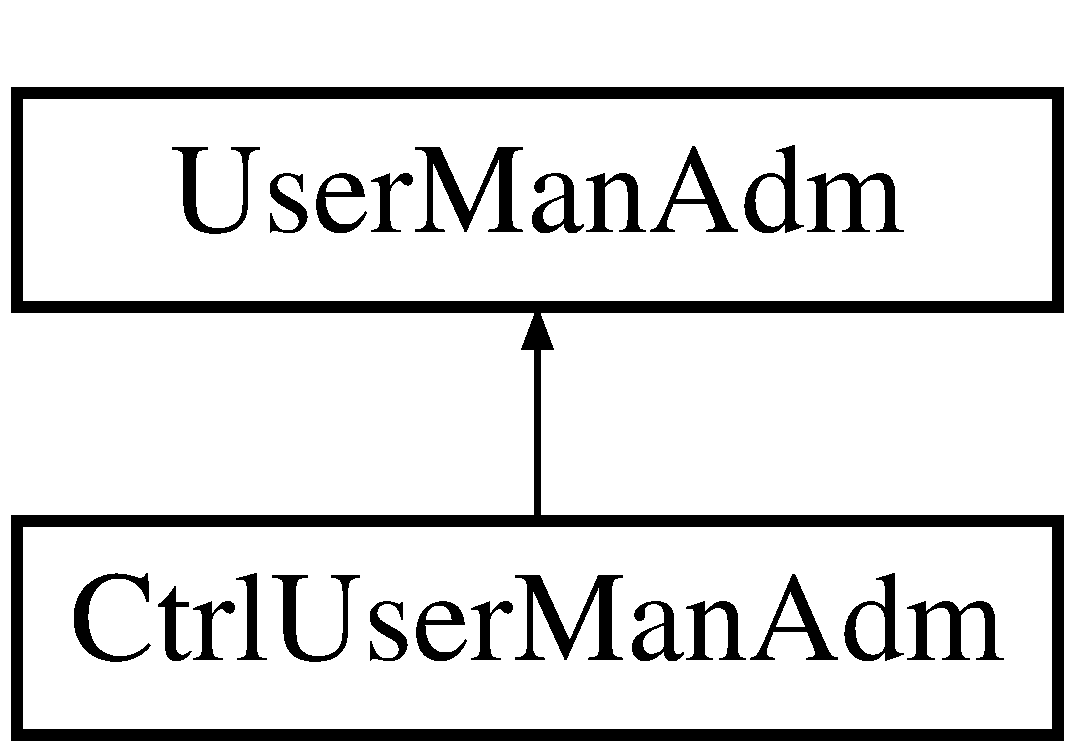
\includegraphics[height=2.000000cm]{d4/d17/classCtrlUserManAdm}
\end{center}
\end{figure}
\subsubsection*{Public Member Functions}
\begin{DoxyCompactItemize}
\item 
void \hyperlink{classCtrlUserManAdm_a90fe4e0ab40e70992e28b0f56bcd76ac}{change\-Password} (\hyperlink{classUsrMatric}{Usr\-Matric}, \hyperlink{classUsrPassword}{Usr\-Password} $\ast$)  throw (\-Pers\-Error)
\begin{DoxyCompactList}\small\item\em Modifica a senha do usuário. \end{DoxyCompactList}\item 
void \hyperlink{classCtrlUserManAdm_ade392e40cc2b451590ef12b2af83674a}{create\-Manager} (\hyperlink{classUsrName}{Usr\-Name} $\ast$, \hyperlink{classUsrPassword}{Usr\-Password} $\ast$)  throw (\-Pers\-Error)
\begin{DoxyCompactList}\small\item\em Cria um novo Gerente. \end{DoxyCompactList}\item 
list$<$ \hyperlink{classManager}{Manager} $>$ \hyperlink{classCtrlUserManAdm_a65dc2eb59bff96b49f6b3bb06ee52fba}{fetch\-Manager} (void)  throw (\-Pers\-Error)
\begin{DoxyCompactList}\small\item\em Recupera uma lista com todos os gerentes registrados no sistema. \end{DoxyCompactList}\item 
\hyperlink{classManager}{Manager} \hyperlink{classCtrlUserManAdm_a45eba11162e5e9090575a8189184bb74}{fetch\-Manager} (\hyperlink{classUsrMatric}{Usr\-Matric})  throw (\-Pers\-Error)
\begin{DoxyCompactList}\small\item\em Recupera os dados de um gerente em específico. \end{DoxyCompactList}\item 
void \hyperlink{classCtrlUserManAdm_a114bc87d024079d6670f8880bd41c908}{edit\-Man\-Name} (\hyperlink{classUsrMatric}{Usr\-Matric} $\ast$, \hyperlink{classUsrName}{Usr\-Name} $\ast$)  throw (invalid\-\_\-argument, Pers\-Error)
\begin{DoxyCompactList}\small\item\em Edita o nome de um gerente. \end{DoxyCompactList}\item 
void \hyperlink{classCtrlUserManAdm_ab8a2c5188f0f90de9bf86d0e50a726e5}{delete\-Manager} (\hyperlink{classUsrMatric}{Usr\-Matric} $\ast$)  throw (invalid\-\_\-argument, Pers\-Error)
\begin{DoxyCompactList}\small\item\em Deleta os dados de um gerente. \end{DoxyCompactList}\end{DoxyCompactItemize}


\subsubsection{Detailed Description}
Classe de negócio para administração de dados de Gerentes e Administradores. 

Definition at line 117 of file User\-Unit.\-h.



\subsubsection{Member Function Documentation}
\hypertarget{classCtrlUserManAdm_a90fe4e0ab40e70992e28b0f56bcd76ac}{\index{Ctrl\-User\-Man\-Adm@{Ctrl\-User\-Man\-Adm}!change\-Password@{change\-Password}}
\index{change\-Password@{change\-Password}!CtrlUserManAdm@{Ctrl\-User\-Man\-Adm}}
\paragraph[{change\-Password}]{\setlength{\rightskip}{0pt plus 5cm}void Ctrl\-User\-Man\-Adm\-::change\-Password (
\begin{DoxyParamCaption}
\item[{{\bf Usr\-Matric}}]{, }
\item[{{\bf Usr\-Password} $\ast$}]{}
\end{DoxyParamCaption}
)  throw ({\bf Pers\-Error})\hspace{0.3cm}{\ttfamily [virtual]}}}\label{d4/d17/classCtrlUserManAdm_a90fe4e0ab40e70992e28b0f56bcd76ac}


Modifica a senha do usuário. 



Implements \hyperlink{classUserManAdm_a063745d21053a5e071ce1f4c6a1c3c55}{User\-Man\-Adm}.



Definition at line 264 of file User\-Unit.\-cpp.

\hypertarget{classCtrlUserManAdm_ade392e40cc2b451590ef12b2af83674a}{\index{Ctrl\-User\-Man\-Adm@{Ctrl\-User\-Man\-Adm}!create\-Manager@{create\-Manager}}
\index{create\-Manager@{create\-Manager}!CtrlUserManAdm@{Ctrl\-User\-Man\-Adm}}
\paragraph[{create\-Manager}]{\setlength{\rightskip}{0pt plus 5cm}void Ctrl\-User\-Man\-Adm\-::create\-Manager (
\begin{DoxyParamCaption}
\item[{{\bf Usr\-Name} $\ast$}]{, }
\item[{{\bf Usr\-Password} $\ast$}]{}
\end{DoxyParamCaption}
)  throw ({\bf Pers\-Error})\hspace{0.3cm}{\ttfamily [virtual]}}}\label{d4/d17/classCtrlUserManAdm_ade392e40cc2b451590ef12b2af83674a}


Cria um novo Gerente. 



Implements \hyperlink{classUserManAdm_a4c1d61e8190867eb786cdf97083ba289}{User\-Man\-Adm}.



Definition at line 271 of file User\-Unit.\-cpp.

\hypertarget{classCtrlUserManAdm_ab8a2c5188f0f90de9bf86d0e50a726e5}{\index{Ctrl\-User\-Man\-Adm@{Ctrl\-User\-Man\-Adm}!delete\-Manager@{delete\-Manager}}
\index{delete\-Manager@{delete\-Manager}!CtrlUserManAdm@{Ctrl\-User\-Man\-Adm}}
\paragraph[{delete\-Manager}]{\setlength{\rightskip}{0pt plus 5cm}void Ctrl\-User\-Man\-Adm\-::delete\-Manager (
\begin{DoxyParamCaption}
\item[{{\bf Usr\-Matric} $\ast$}]{}
\end{DoxyParamCaption}
)  throw (invalid\-\_\-argument, {\bf Pers\-Error})\hspace{0.3cm}{\ttfamily [virtual]}}}\label{d4/d17/classCtrlUserManAdm_ab8a2c5188f0f90de9bf86d0e50a726e5}


Deleta os dados de um gerente. 



Implements \hyperlink{classUserManAdm_a3fd6ddb6b71743fe5ece3100206023c3}{User\-Man\-Adm}.



Definition at line 319 of file User\-Unit.\-cpp.

\hypertarget{classCtrlUserManAdm_a114bc87d024079d6670f8880bd41c908}{\index{Ctrl\-User\-Man\-Adm@{Ctrl\-User\-Man\-Adm}!edit\-Man\-Name@{edit\-Man\-Name}}
\index{edit\-Man\-Name@{edit\-Man\-Name}!CtrlUserManAdm@{Ctrl\-User\-Man\-Adm}}
\paragraph[{edit\-Man\-Name}]{\setlength{\rightskip}{0pt plus 5cm}void Ctrl\-User\-Man\-Adm\-::edit\-Man\-Name (
\begin{DoxyParamCaption}
\item[{{\bf Usr\-Matric} $\ast$}]{, }
\item[{{\bf Usr\-Name} $\ast$}]{}
\end{DoxyParamCaption}
)  throw (invalid\-\_\-argument, {\bf Pers\-Error})\hspace{0.3cm}{\ttfamily [virtual]}}}\label{d4/d17/classCtrlUserManAdm_a114bc87d024079d6670f8880bd41c908}


Edita o nome de um gerente. 

Sua matrícula não será afetada 

Implements \hyperlink{classUserManAdm_a0440de1c9d712a8dac1aa4e526d0fe9b}{User\-Man\-Adm}.



Definition at line 306 of file User\-Unit.\-cpp.

\hypertarget{classCtrlUserManAdm_a65dc2eb59bff96b49f6b3bb06ee52fba}{\index{Ctrl\-User\-Man\-Adm@{Ctrl\-User\-Man\-Adm}!fetch\-Manager@{fetch\-Manager}}
\index{fetch\-Manager@{fetch\-Manager}!CtrlUserManAdm@{Ctrl\-User\-Man\-Adm}}
\paragraph[{fetch\-Manager}]{\setlength{\rightskip}{0pt plus 5cm}list$<$ {\bf Manager} $>$ Ctrl\-User\-Man\-Adm\-::fetch\-Manager (
\begin{DoxyParamCaption}
\item[{void}]{}
\end{DoxyParamCaption}
)  throw ({\bf Pers\-Error})\hspace{0.3cm}{\ttfamily [virtual]}}}\label{d4/d17/classCtrlUserManAdm_a65dc2eb59bff96b49f6b3bb06ee52fba}


Recupera uma lista com todos os gerentes registrados no sistema. 



Implements \hyperlink{classUserManAdm_a05b8b4f5b1e42b7b9f77d6a40b90dbb2}{User\-Man\-Adm}.



Definition at line 288 of file User\-Unit.\-cpp.

\hypertarget{classCtrlUserManAdm_a45eba11162e5e9090575a8189184bb74}{\index{Ctrl\-User\-Man\-Adm@{Ctrl\-User\-Man\-Adm}!fetch\-Manager@{fetch\-Manager}}
\index{fetch\-Manager@{fetch\-Manager}!CtrlUserManAdm@{Ctrl\-User\-Man\-Adm}}
\paragraph[{fetch\-Manager}]{\setlength{\rightskip}{0pt plus 5cm}{\bf Manager} Ctrl\-User\-Man\-Adm\-::fetch\-Manager (
\begin{DoxyParamCaption}
\item[{{\bf Usr\-Matric}}]{}
\end{DoxyParamCaption}
)  throw ({\bf Pers\-Error})\hspace{0.3cm}{\ttfamily [virtual]}}}\label{d4/d17/classCtrlUserManAdm_a45eba11162e5e9090575a8189184bb74}


Recupera os dados de um gerente em específico. 



Implements \hyperlink{classUserManAdm_a62e826d1c11061df021016e94e88f9ba}{User\-Man\-Adm}.



Definition at line 297 of file User\-Unit.\-cpp.



The documentation for this class was generated from the following files\-:\begin{DoxyCompactItemize}
\item 
User\-Unit.\-h\item 
User\-Unit.\-cpp\end{DoxyCompactItemize}

\hypertarget{classCustomer}{\subsection{Customer Class Reference}
\label{d9/d12/classCustomer}\index{Customer@{Customer}}
}


Cliente; Onde ficarão armazenados os dados do usuário padrão do sistema.  




{\ttfamily \#include $<$Entity\-Unit.\-h$>$}

Inheritance diagram for Customer\-:\begin{figure}[H]
\begin{center}
\leavevmode
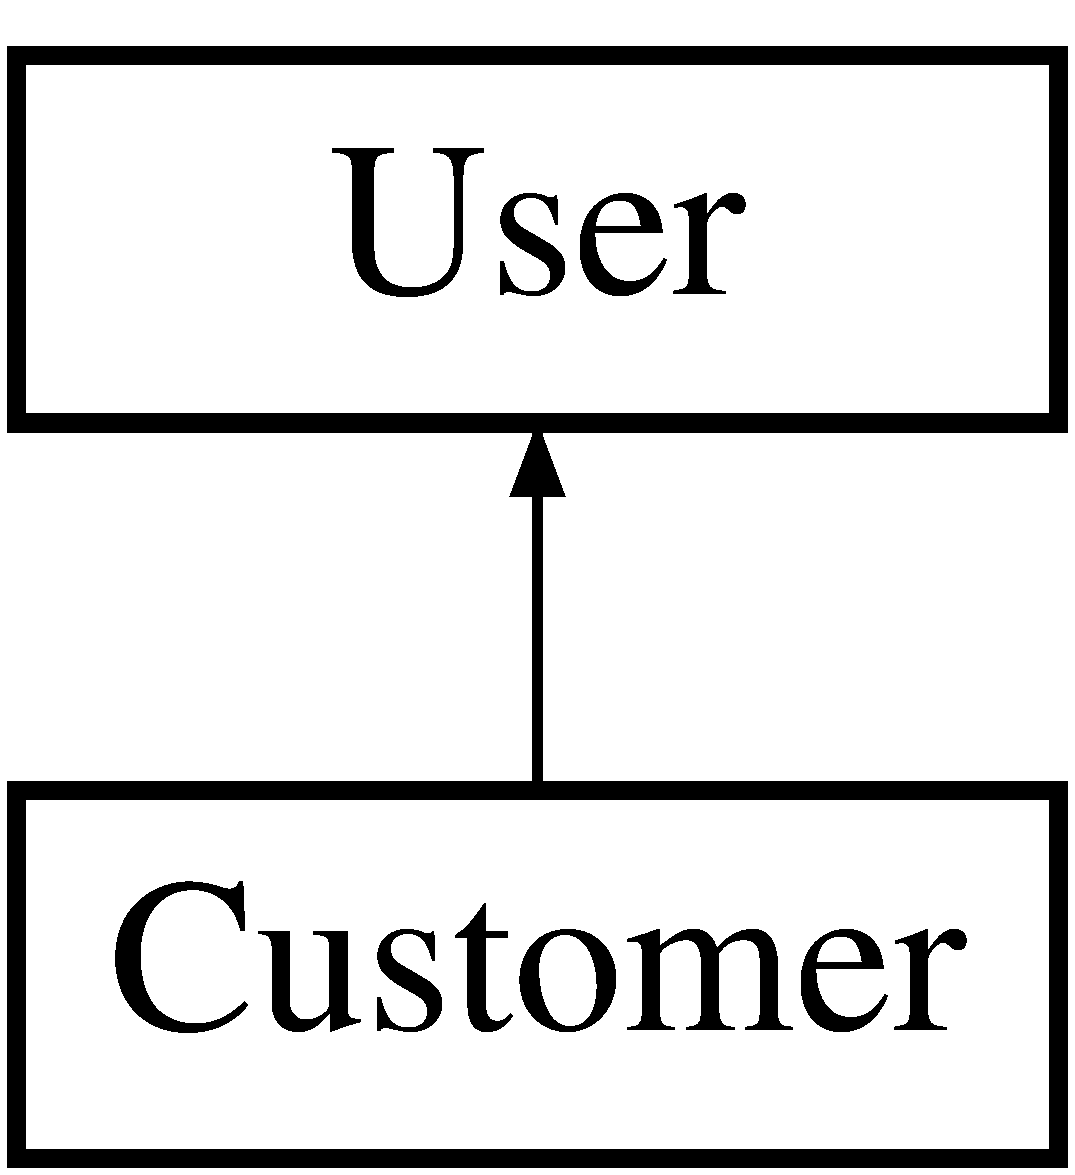
\includegraphics[height=2.000000cm]{d9/d12/classCustomer}
\end{center}
\end{figure}
\subsubsection*{Public Member Functions}
\begin{DoxyCompactItemize}
\item 
\hyperlink{classCustomer_a3f3be282d21b234e1e72f645d8fdc362}{Customer} (const \hyperlink{classUsrName}{Usr\-Name} \&, const \hyperlink{classUsrPassword}{Usr\-Password} \&, const \hyperlink{classUsrId}{Usr\-Id} \&)
\begin{DoxyCompactList}\small\item\em Construtor base de \hyperlink{classCustomer}{Customer}. \end{DoxyCompactList}\item 
\hyperlink{classUsrId}{Usr\-Id} \hyperlink{classCustomer_a76d325591ef27599cb1d7f3e4b77b8d4}{get\-Usr\-Id} () const 
\begin{DoxyCompactList}\small\item\em Método que recupera o valor contido no campo usr\-Id. \end{DoxyCompactList}\item 
void \hyperlink{classCustomer_a89b74269a4750193d61b305b13df82fa}{set\-Usr\-Id} (const \hyperlink{classUsrId}{Usr\-Id} \&)
\begin{DoxyCompactList}\small\item\em Método que define o valor do atributo usr\-Id. \end{DoxyCompactList}\end{DoxyCompactItemize}
\subsubsection*{Additional Inherited Members}


\subsubsection{Detailed Description}
Cliente; Onde ficarão armazenados os dados do usuário padrão do sistema. 

O \hyperlink{classCustomer}{Customer} (Cliente) terá acesso a uma ou mais contas através de um \hyperlink{classUsrId}{Usr\-Id} único. Através dessa(s) conta(s), é capaz de realizar transações. 

Definition at line 40 of file Entity\-Unit.\-h.



\subsubsection{Constructor \& Destructor Documentation}
\hypertarget{classCustomer_a3f3be282d21b234e1e72f645d8fdc362}{\index{Customer@{Customer}!Customer@{Customer}}
\index{Customer@{Customer}!Customer@{Customer}}
\paragraph[{Customer}]{\setlength{\rightskip}{0pt plus 5cm}Customer\-::\-Customer (
\begin{DoxyParamCaption}
\item[{const {\bf Usr\-Name} \&}]{name, }
\item[{const {\bf Usr\-Password} \&}]{password, }
\item[{const {\bf Usr\-Id} \&}]{usr\-Id}
\end{DoxyParamCaption}
)}}\label{d9/d12/classCustomer_a3f3be282d21b234e1e72f645d8fdc362}


Construtor base de \hyperlink{classCustomer}{Customer}. 

Define os valores internos da classe automaticamente. 

Definition at line 17 of file Entity\-Unit.\-cpp.



\subsubsection{Member Function Documentation}
\hypertarget{classCustomer_a76d325591ef27599cb1d7f3e4b77b8d4}{\index{Customer@{Customer}!get\-Usr\-Id@{get\-Usr\-Id}}
\index{get\-Usr\-Id@{get\-Usr\-Id}!Customer@{Customer}}
\paragraph[{get\-Usr\-Id}]{\setlength{\rightskip}{0pt plus 5cm}{\bf Usr\-Id} Customer\-::get\-Usr\-Id (
\begin{DoxyParamCaption}
{}
\end{DoxyParamCaption}
) const\hspace{0.3cm}{\ttfamily [inline]}}}\label{d9/d12/classCustomer_a76d325591ef27599cb1d7f3e4b77b8d4}


Método que recupera o valor contido no campo usr\-Id. 

O valor é retornado, e o atributo não é modificado no processo. 

Definition at line 59 of file Entity\-Unit.\-h.

\hypertarget{classCustomer_a89b74269a4750193d61b305b13df82fa}{\index{Customer@{Customer}!set\-Usr\-Id@{set\-Usr\-Id}}
\index{set\-Usr\-Id@{set\-Usr\-Id}!Customer@{Customer}}
\paragraph[{set\-Usr\-Id}]{\setlength{\rightskip}{0pt plus 5cm}void Customer\-::set\-Usr\-Id (
\begin{DoxyParamCaption}
\item[{const {\bf Usr\-Id} \&}]{usr\-Id}
\end{DoxyParamCaption}
)}}\label{d9/d12/classCustomer_a89b74269a4750193d61b305b13df82fa}


Método que define o valor do atributo usr\-Id. 



Definition at line 24 of file Entity\-Unit.\-cpp.



The documentation for this class was generated from the following files\-:\begin{DoxyCompactItemize}
\item 
Entity\-Unit.\-h\item 
Entity\-Unit.\-cpp\end{DoxyCompactItemize}

\hypertarget{classMainAdmMenu}{\section{Main\-Adm\-Menu Class Reference}
\label{d9/d86/classMainAdmMenu}\index{Main\-Adm\-Menu@{Main\-Adm\-Menu}}
}


Menu principal para administradores.  




{\ttfamily \#include $<$Main\-Unit.\-h$>$}

Inheritance diagram for Main\-Adm\-Menu\-:\begin{figure}[H]
\begin{center}
\leavevmode
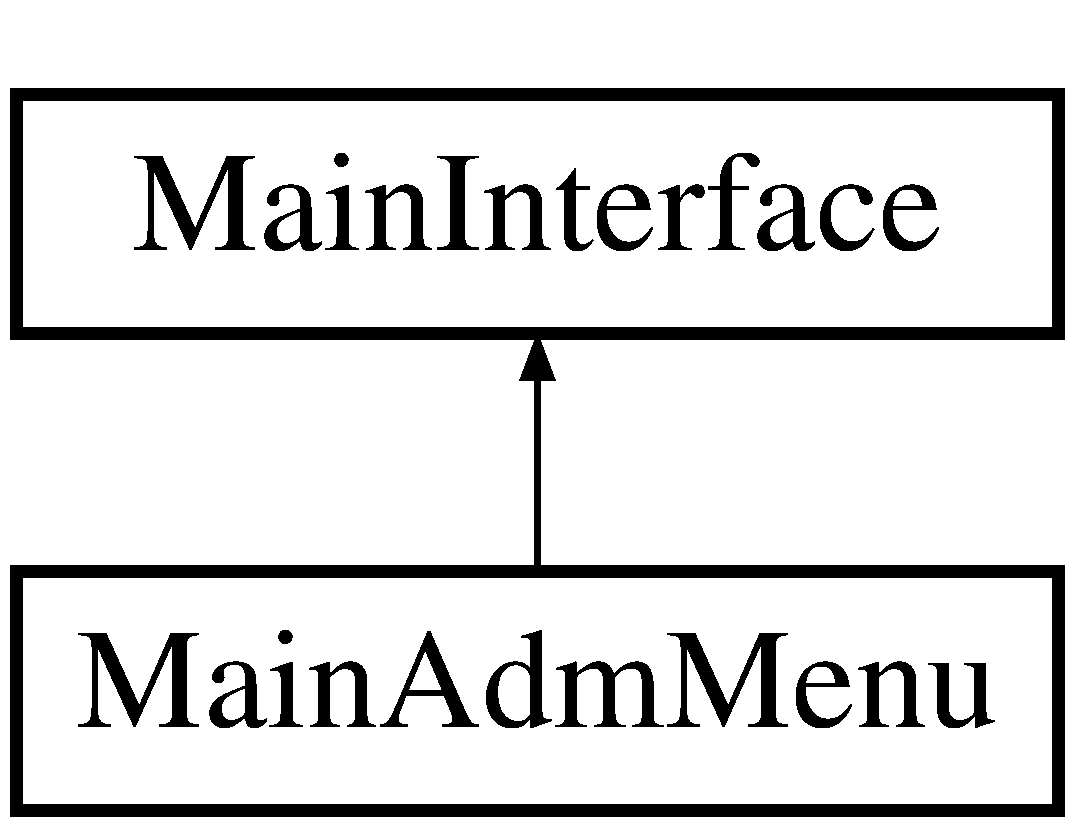
\includegraphics[height=2.000000cm]{d9/d86/classMainAdmMenu}
\end{center}
\end{figure}
\subsection*{Public Member Functions}
\begin{DoxyCompactItemize}
\item 
void \hyperlink{classMainAdmMenu_aa0c46ea4cc61cddfc75e7eb03f549832}{execute} ()
\begin{DoxyCompactList}\small\item\em Passa o controle do programa para a classe em questão. \end{DoxyCompactList}\item 
void \hyperlink{classMainAdmMenu_a86c57f1f8d9762ee6efbadef3f990f67}{set\-User\-Adm} (\hyperlink{classUserManAdm}{User\-Man\-Adm} $\ast$)
\begin{DoxyCompactList}\small\item\em Define o objeto de negócio. \end{DoxyCompactList}\end{DoxyCompactItemize}


\subsection{Detailed Description}
Menu principal para administradores. 

Através dele tem-\/se acesso aos dados cadastrais de todos os gerentes. 

\subsection{Member Function Documentation}
\hypertarget{classMainAdmMenu_aa0c46ea4cc61cddfc75e7eb03f549832}{\index{Main\-Adm\-Menu@{Main\-Adm\-Menu}!execute@{execute}}
\index{execute@{execute}!MainAdmMenu@{Main\-Adm\-Menu}}
\subsubsection[{execute}]{\setlength{\rightskip}{0pt plus 5cm}void Main\-Adm\-Menu\-::execute (
\begin{DoxyParamCaption}
{}
\end{DoxyParamCaption}
)\hspace{0.3cm}{\ttfamily [virtual]}}}\label{d9/d86/classMainAdmMenu_aa0c46ea4cc61cddfc75e7eb03f549832}


Passa o controle do programa para a classe em questão. 



Implements \hyperlink{classMainInterface_a9cf3c80db93173916d14a996d9a29398}{Main\-Interface}.

\hypertarget{classMainAdmMenu_a86c57f1f8d9762ee6efbadef3f990f67}{\index{Main\-Adm\-Menu@{Main\-Adm\-Menu}!set\-User\-Adm@{set\-User\-Adm}}
\index{set\-User\-Adm@{set\-User\-Adm}!MainAdmMenu@{Main\-Adm\-Menu}}
\subsubsection[{set\-User\-Adm}]{\setlength{\rightskip}{0pt plus 5cm}void Main\-Adm\-Menu\-::set\-User\-Adm (
\begin{DoxyParamCaption}
\item[{{\bf User\-Man\-Adm} $\ast$}]{user\-Adm}
\end{DoxyParamCaption}
)\hspace{0.3cm}{\ttfamily [inline]}}}\label{d9/d86/classMainAdmMenu_a86c57f1f8d9762ee6efbadef3f990f67}


Define o objeto de negócio. 



The documentation for this class was generated from the following files\-:\begin{DoxyCompactItemize}
\item 
Main\-Unit.\-h\item 
Main\-Unit.\-cpp\end{DoxyCompactItemize}

\hypertarget{classMainCusMenu}{\section{Main\-Cus\-Menu Class Reference}
\label{dc/d35/classMainCusMenu}\index{Main\-Cus\-Menu@{Main\-Cus\-Menu}}
}


Menu principal para Clientes.  




{\ttfamily \#include $<$Main\-Unit.\-h$>$}

Inheritance diagram for Main\-Cus\-Menu\-:\begin{figure}[H]
\begin{center}
\leavevmode
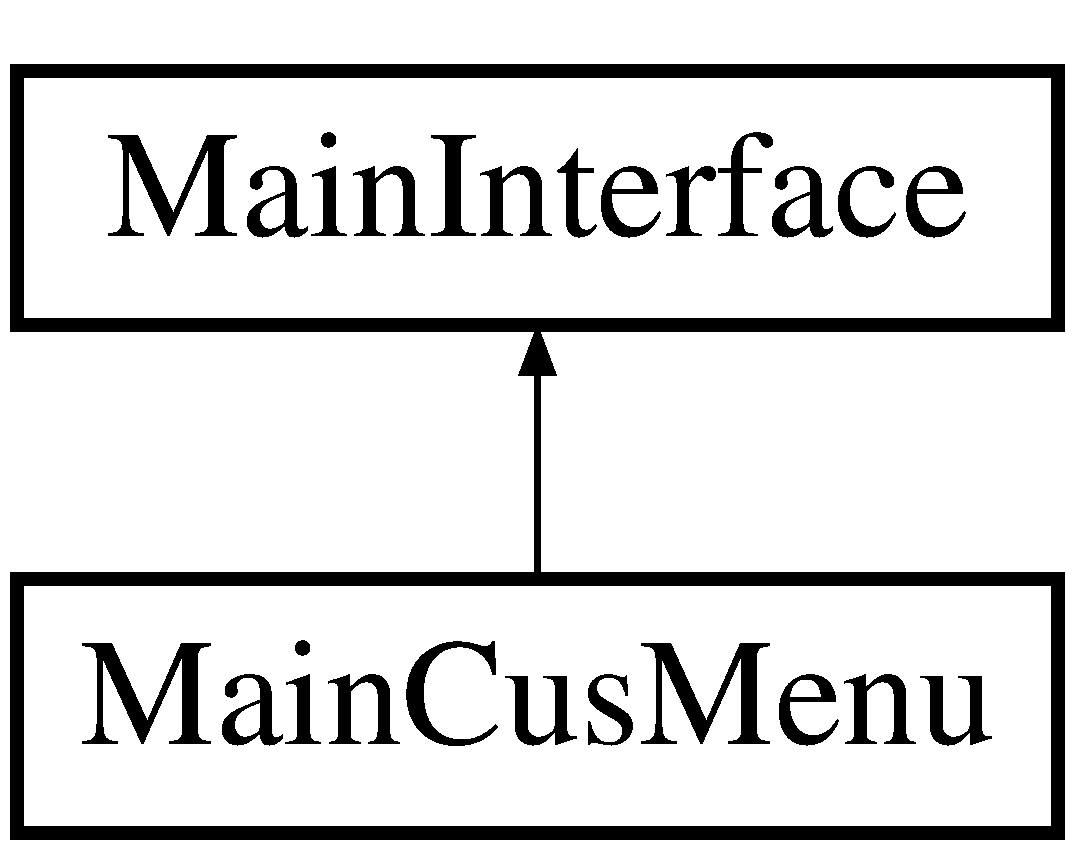
\includegraphics[height=2.000000cm]{dc/d35/classMainCusMenu}
\end{center}
\end{figure}
\subsection*{Public Member Functions}
\begin{DoxyCompactItemize}
\item 
void \hyperlink{classMainCusMenu_a91a3ffa75a1deb30dfc6eb604f1a1a2d}{execute} ()
\begin{DoxyCompactList}\small\item\em Passa o controle do programa para a classe em questão. \end{DoxyCompactList}\item 
void \hyperlink{classMainCusMenu_aea07e41b2f2c24496e3ce7a8f55b5332}{set\-User\-Adm} (\hyperlink{classUserCusAdm}{User\-Cus\-Adm} $\ast$)
\begin{DoxyCompactList}\small\item\em Define a classe responsável pela edição de dados de clientes. \end{DoxyCompactList}\item 
void \hyperlink{classMainCusMenu_acaa0828f9ac38816e5a6068f1781f9be}{set\-Acc\-Adm} (\hyperlink{classUserAccAdm}{User\-Acc\-Adm} $\ast$)
\begin{DoxyCompactList}\small\item\em Define a classe responsável pela edição de dados de contas. \end{DoxyCompactList}\item 
void \hyperlink{classMainCusMenu_aa338655efeeb61c43a8089c5577ce47b}{set\-Transac\-Adm} (\hyperlink{classTransacAdm}{Transac\-Adm} $\ast$)
\begin{DoxyCompactList}\small\item\em Define a classe responsável pelo intermédio de transações entre contas. \end{DoxyCompactList}\end{DoxyCompactItemize}


\subsection{Detailed Description}
Menu principal para Clientes. 

Através dele tem-\/se acesso aos pagamentos e dinheiro associados à conta do cliente logado. 

\subsection{Member Function Documentation}
\hypertarget{classMainCusMenu_a91a3ffa75a1deb30dfc6eb604f1a1a2d}{\index{Main\-Cus\-Menu@{Main\-Cus\-Menu}!execute@{execute}}
\index{execute@{execute}!MainCusMenu@{Main\-Cus\-Menu}}
\subsubsection[{execute}]{\setlength{\rightskip}{0pt plus 5cm}void Main\-Cus\-Menu\-::execute (
\begin{DoxyParamCaption}
{}
\end{DoxyParamCaption}
)\hspace{0.3cm}{\ttfamily [virtual]}}}\label{dc/d35/classMainCusMenu_a91a3ffa75a1deb30dfc6eb604f1a1a2d}


Passa o controle do programa para a classe em questão. 



Implements \hyperlink{classMainInterface_a9cf3c80db93173916d14a996d9a29398}{Main\-Interface}.

\hypertarget{classMainCusMenu_acaa0828f9ac38816e5a6068f1781f9be}{\index{Main\-Cus\-Menu@{Main\-Cus\-Menu}!set\-Acc\-Adm@{set\-Acc\-Adm}}
\index{set\-Acc\-Adm@{set\-Acc\-Adm}!MainCusMenu@{Main\-Cus\-Menu}}
\subsubsection[{set\-Acc\-Adm}]{\setlength{\rightskip}{0pt plus 5cm}void Main\-Cus\-Menu\-::set\-Acc\-Adm (
\begin{DoxyParamCaption}
\item[{{\bf User\-Acc\-Adm} $\ast$}]{acc\-Adm}
\end{DoxyParamCaption}
)\hspace{0.3cm}{\ttfamily [inline]}}}\label{dc/d35/classMainCusMenu_acaa0828f9ac38816e5a6068f1781f9be}


Define a classe responsável pela edição de dados de contas. 

\hypertarget{classMainCusMenu_aa338655efeeb61c43a8089c5577ce47b}{\index{Main\-Cus\-Menu@{Main\-Cus\-Menu}!set\-Transac\-Adm@{set\-Transac\-Adm}}
\index{set\-Transac\-Adm@{set\-Transac\-Adm}!MainCusMenu@{Main\-Cus\-Menu}}
\subsubsection[{set\-Transac\-Adm}]{\setlength{\rightskip}{0pt plus 5cm}void Main\-Cus\-Menu\-::set\-Transac\-Adm (
\begin{DoxyParamCaption}
\item[{{\bf Transac\-Adm} $\ast$}]{transac\-Adm}
\end{DoxyParamCaption}
)\hspace{0.3cm}{\ttfamily [inline]}}}\label{dc/d35/classMainCusMenu_aa338655efeeb61c43a8089c5577ce47b}


Define a classe responsável pelo intermédio de transações entre contas. 

\hypertarget{classMainCusMenu_aea07e41b2f2c24496e3ce7a8f55b5332}{\index{Main\-Cus\-Menu@{Main\-Cus\-Menu}!set\-User\-Adm@{set\-User\-Adm}}
\index{set\-User\-Adm@{set\-User\-Adm}!MainCusMenu@{Main\-Cus\-Menu}}
\subsubsection[{set\-User\-Adm}]{\setlength{\rightskip}{0pt plus 5cm}void Main\-Cus\-Menu\-::set\-User\-Adm (
\begin{DoxyParamCaption}
\item[{{\bf User\-Cus\-Adm} $\ast$}]{user\-Adm}
\end{DoxyParamCaption}
)\hspace{0.3cm}{\ttfamily [inline]}}}\label{dc/d35/classMainCusMenu_aea07e41b2f2c24496e3ce7a8f55b5332}


Define a classe responsável pela edição de dados de clientes. 



The documentation for this class was generated from the following files\-:\begin{DoxyCompactItemize}
\item 
Main\-Unit.\-h\item 
Main\-Unit.\-cpp\end{DoxyCompactItemize}

\hypertarget{classMainInterface}{\section{Main\-Interface Class Reference}
\label{d2/da2/classMainInterface}\index{Main\-Interface@{Main\-Interface}}
}


Interface base para criação das classes da camada de apresentação.  




{\ttfamily \#include $<$Main\-Unit.\-h$>$}

Inheritance diagram for Main\-Interface\-:\begin{figure}[H]
\begin{center}
\leavevmode
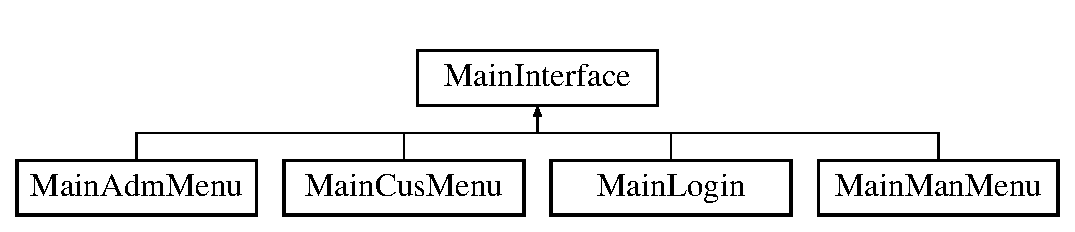
\includegraphics[height=2.000000cm]{d2/da2/classMainInterface}
\end{center}
\end{figure}
\subsection*{Public Member Functions}
\begin{DoxyCompactItemize}
\item 
virtual void \hyperlink{classMainInterface_a9cf3c80db93173916d14a996d9a29398}{execute} ()=0
\begin{DoxyCompactList}\small\item\em Passa o controle do programa para a classe em questão. \end{DoxyCompactList}\end{DoxyCompactItemize}


\subsection{Detailed Description}
Interface base para criação das classes da camada de apresentação. 



\subsection{Member Function Documentation}
\hypertarget{classMainInterface_a9cf3c80db93173916d14a996d9a29398}{\index{Main\-Interface@{Main\-Interface}!execute@{execute}}
\index{execute@{execute}!MainInterface@{Main\-Interface}}
\subsubsection[{execute}]{\setlength{\rightskip}{0pt plus 5cm}virtual void Main\-Interface\-::execute (
\begin{DoxyParamCaption}
{}
\end{DoxyParamCaption}
)\hspace{0.3cm}{\ttfamily [pure virtual]}}}\label{d2/da2/classMainInterface_a9cf3c80db93173916d14a996d9a29398}


Passa o controle do programa para a classe em questão. 



Implemented in \hyperlink{classMainLogin_ab0149573d015f41f401cfb28aea35509}{Main\-Login}, \hyperlink{classMainCusMenu_a91a3ffa75a1deb30dfc6eb604f1a1a2d}{Main\-Cus\-Menu}, \hyperlink{classMainManMenu_ac864c18863c5f308d0b9c52c223b4b9c}{Main\-Man\-Menu}, and \hyperlink{classMainAdmMenu_aa0c46ea4cc61cddfc75e7eb03f549832}{Main\-Adm\-Menu}.



The documentation for this class was generated from the following file\-:\begin{DoxyCompactItemize}
\item 
Main\-Unit.\-h\end{DoxyCompactItemize}

\hypertarget{classMainLogin}{\subsection{Main\-Login Class Reference}
\label{db/df3/classMainLogin}\index{Main\-Login@{Main\-Login}}
}


Responsável pela execução do login do usuário.  




{\ttfamily \#include $<$Main\-Unit.\-h$>$}

Inheritance diagram for Main\-Login\-:\begin{figure}[H]
\begin{center}
\leavevmode
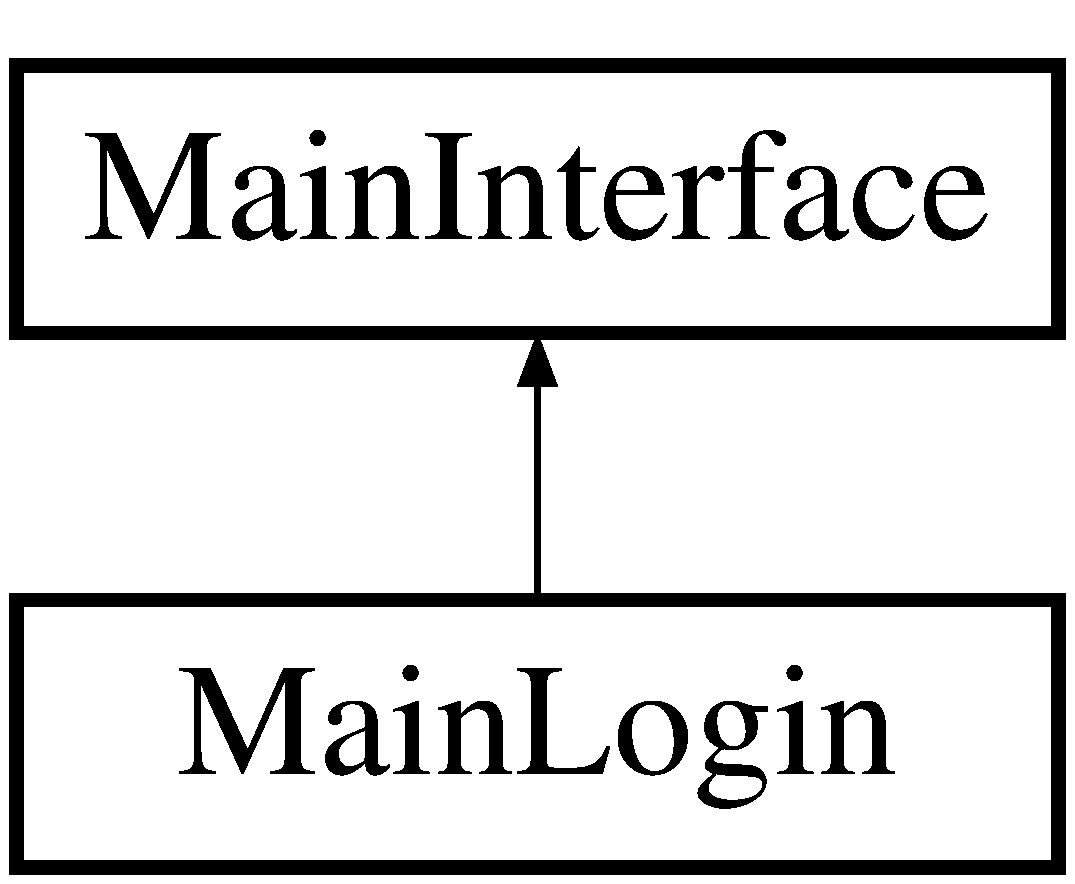
\includegraphics[height=2.000000cm]{db/df3/classMainLogin}
\end{center}
\end{figure}
\subsubsection*{Public Member Functions}
\begin{DoxyCompactItemize}
\item 
void \hyperlink{classMainLogin_ab0149573d015f41f401cfb28aea35509}{execute} ()
\begin{DoxyCompactList}\small\item\em Passa o controle do programa para a classe em questão. \end{DoxyCompactList}\item 
void \hyperlink{classMainLogin_a286c0703647c7c252093bf7589f63c64}{set\-User\-Login} (\hyperlink{classUserLogin}{User\-Login} $\ast$)
\begin{DoxyCompactList}\small\item\em Define a classe responsável pelo negócio. \end{DoxyCompactList}\item 
void \hyperlink{classMainLogin_a0161cf5b7b4d5d829292a38e4059abb5}{set\-Main\-Adm\-Menu} (\hyperlink{classMainAdmMenu}{Main\-Adm\-Menu} $\ast$)
\begin{DoxyCompactList}\small\item\em Define a classe responsável pela execução do menu de Administrador. \end{DoxyCompactList}\item 
void \hyperlink{classMainLogin_a4561c5838a48ad8436cd8d0b1749511a}{set\-Main\-Man\-Menu} (\hyperlink{classMainManMenu}{Main\-Man\-Menu} $\ast$)
\begin{DoxyCompactList}\small\item\em Define a classe responsável pela execução do menu de Gerente. \end{DoxyCompactList}\item 
void \hyperlink{classMainLogin_a2302b88c01b0ea4b29e4a824c5b7f185}{set\-Main\-Cus\-Menu} (\hyperlink{classMainCusMenu}{Main\-Cus\-Menu} $\ast$)
\begin{DoxyCompactList}\small\item\em Define a classe responsável pela execução do menu de Clinete. \end{DoxyCompactList}\end{DoxyCompactItemize}


\subsubsection{Detailed Description}
Responsável pela execução do login do usuário. 



Definition at line 220 of file Main\-Unit.\-h.



\subsubsection{Member Function Documentation}
\hypertarget{classMainLogin_ab0149573d015f41f401cfb28aea35509}{\index{Main\-Login@{Main\-Login}!execute@{execute}}
\index{execute@{execute}!MainLogin@{Main\-Login}}
\paragraph[{execute}]{\setlength{\rightskip}{0pt plus 5cm}void Main\-Login\-::execute (
\begin{DoxyParamCaption}
{}
\end{DoxyParamCaption}
)\hspace{0.3cm}{\ttfamily [virtual]}}}\label{db/df3/classMainLogin_ab0149573d015f41f401cfb28aea35509}


Passa o controle do programa para a classe em questão. 



Implements \hyperlink{classMainInterface_a9cf3c80db93173916d14a996d9a29398}{Main\-Interface}.



Definition at line 63 of file Main\-Unit.\-cpp.

\hypertarget{classMainLogin_a0161cf5b7b4d5d829292a38e4059abb5}{\index{Main\-Login@{Main\-Login}!set\-Main\-Adm\-Menu@{set\-Main\-Adm\-Menu}}
\index{set\-Main\-Adm\-Menu@{set\-Main\-Adm\-Menu}!MainLogin@{Main\-Login}}
\paragraph[{set\-Main\-Adm\-Menu}]{\setlength{\rightskip}{0pt plus 5cm}void Main\-Login\-::set\-Main\-Adm\-Menu (
\begin{DoxyParamCaption}
\item[{{\bf Main\-Adm\-Menu} $\ast$}]{adm\-Menu}
\end{DoxyParamCaption}
)\hspace{0.3cm}{\ttfamily [inline]}}}\label{db/df3/classMainLogin_a0161cf5b7b4d5d829292a38e4059abb5}


Define a classe responsável pela execução do menu de Administrador. 



Definition at line 259 of file Main\-Unit.\-h.

\hypertarget{classMainLogin_a2302b88c01b0ea4b29e4a824c5b7f185}{\index{Main\-Login@{Main\-Login}!set\-Main\-Cus\-Menu@{set\-Main\-Cus\-Menu}}
\index{set\-Main\-Cus\-Menu@{set\-Main\-Cus\-Menu}!MainLogin@{Main\-Login}}
\paragraph[{set\-Main\-Cus\-Menu}]{\setlength{\rightskip}{0pt plus 5cm}void Main\-Login\-::set\-Main\-Cus\-Menu (
\begin{DoxyParamCaption}
\item[{{\bf Main\-Cus\-Menu} $\ast$}]{cus\-Menu}
\end{DoxyParamCaption}
)\hspace{0.3cm}{\ttfamily [inline]}}}\label{db/df3/classMainLogin_a2302b88c01b0ea4b29e4a824c5b7f185}


Define a classe responsável pela execução do menu de Clinete. 



Definition at line 269 of file Main\-Unit.\-h.

\hypertarget{classMainLogin_a4561c5838a48ad8436cd8d0b1749511a}{\index{Main\-Login@{Main\-Login}!set\-Main\-Man\-Menu@{set\-Main\-Man\-Menu}}
\index{set\-Main\-Man\-Menu@{set\-Main\-Man\-Menu}!MainLogin@{Main\-Login}}
\paragraph[{set\-Main\-Man\-Menu}]{\setlength{\rightskip}{0pt plus 5cm}void Main\-Login\-::set\-Main\-Man\-Menu (
\begin{DoxyParamCaption}
\item[{{\bf Main\-Man\-Menu} $\ast$}]{man\-Menu}
\end{DoxyParamCaption}
)\hspace{0.3cm}{\ttfamily [inline]}}}\label{db/df3/classMainLogin_a4561c5838a48ad8436cd8d0b1749511a}


Define a classe responsável pela execução do menu de Gerente. 



Definition at line 264 of file Main\-Unit.\-h.

\hypertarget{classMainLogin_a286c0703647c7c252093bf7589f63c64}{\index{Main\-Login@{Main\-Login}!set\-User\-Login@{set\-User\-Login}}
\index{set\-User\-Login@{set\-User\-Login}!MainLogin@{Main\-Login}}
\paragraph[{set\-User\-Login}]{\setlength{\rightskip}{0pt plus 5cm}void Main\-Login\-::set\-User\-Login (
\begin{DoxyParamCaption}
\item[{{\bf User\-Login} $\ast$}]{user\-Login}
\end{DoxyParamCaption}
)\hspace{0.3cm}{\ttfamily [inline]}}}\label{db/df3/classMainLogin_a286c0703647c7c252093bf7589f63c64}


Define a classe responsável pelo negócio. 



Definition at line 254 of file Main\-Unit.\-h.



The documentation for this class was generated from the following files\-:\begin{DoxyCompactItemize}
\item 
Main\-Unit.\-h\item 
Main\-Unit.\-cpp\end{DoxyCompactItemize}

\hypertarget{classMainManMenu}{\subsection{Main\-Man\-Menu Class Reference}
\label{d0/d1d/classMainManMenu}\index{Main\-Man\-Menu@{Main\-Man\-Menu}}
}


Menu principal para Gerentes.  




{\ttfamily \#include $<$Main\-Unit.\-h$>$}

Inheritance diagram for Main\-Man\-Menu\-:\begin{figure}[H]
\begin{center}
\leavevmode
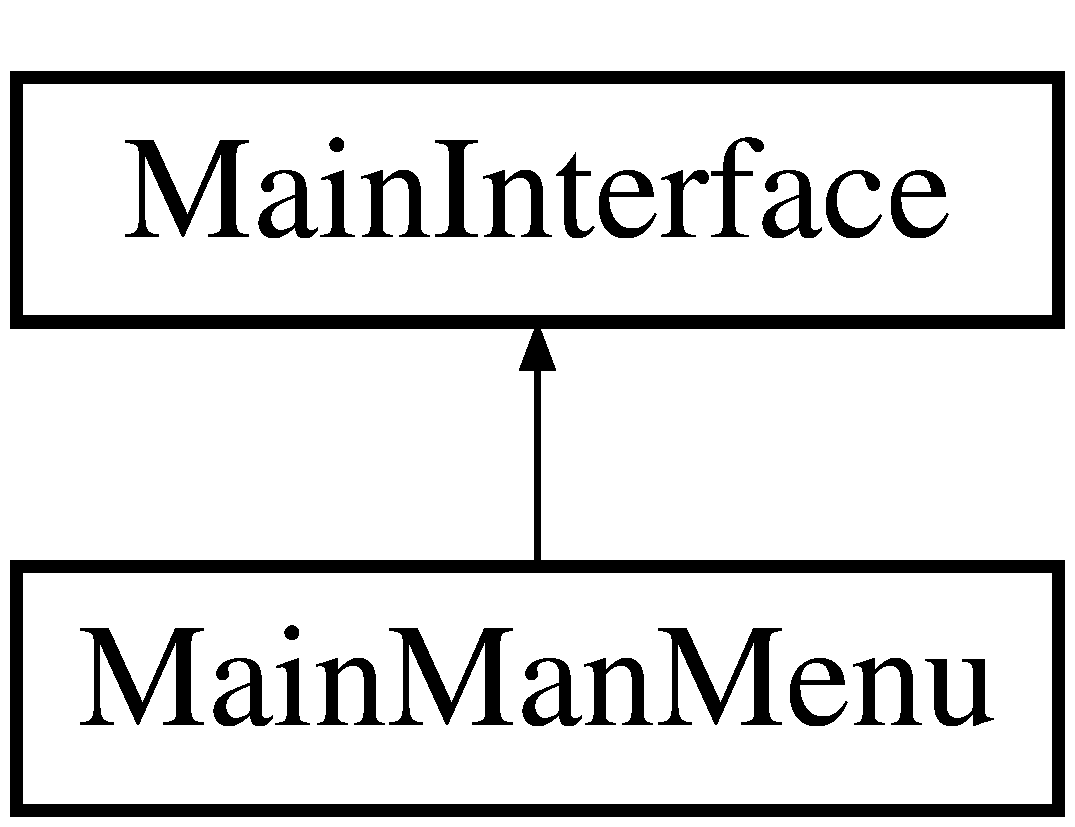
\includegraphics[height=2.000000cm]{d0/d1d/classMainManMenu}
\end{center}
\end{figure}
\subsubsection*{Public Member Functions}
\begin{DoxyCompactItemize}
\item 
void \hyperlink{classMainManMenu_ac864c18863c5f308d0b9c52c223b4b9c}{execute} ()
\begin{DoxyCompactList}\small\item\em Passa o controle do programa para a classe em questão. \end{DoxyCompactList}\item 
void \hyperlink{classMainManMenu_aa4174687e0614fd63783c39340dfc17e}{set\-User\-Adm} (\hyperlink{classUserManAdm}{User\-Man\-Adm} $\ast$)
\begin{DoxyCompactList}\small\item\em Define o objeto de negócio para administração de dados de gerente. \end{DoxyCompactList}\item 
void \hyperlink{classMainManMenu_a507ebea41371d58e137ece5a11bb63bf}{set\-Acc\-Adm} (\hyperlink{classUserAccAdm}{User\-Acc\-Adm} $\ast$)
\begin{DoxyCompactList}\small\item\em Define o objeto de negócio para administração de dados de conta. \end{DoxyCompactList}\item 
void \hyperlink{classMainManMenu_a94b488d911497cf9453e9277806d5241}{set\-Cus\-Adm} (\hyperlink{classUserCusAdm}{User\-Cus\-Adm} $\ast$)
\begin{DoxyCompactList}\small\item\em Define o objeto de negócio para administração de dados de cliente. \end{DoxyCompactList}\end{DoxyCompactItemize}


\subsubsection{Detailed Description}
Menu principal para Gerentes. 

Através dele tem-\/se acesso aos dados cadastrais de todas as contas. 

Definition at line 83 of file Main\-Unit.\-h.



\subsubsection{Member Function Documentation}
\hypertarget{classMainManMenu_ac864c18863c5f308d0b9c52c223b4b9c}{\index{Main\-Man\-Menu@{Main\-Man\-Menu}!execute@{execute}}
\index{execute@{execute}!MainManMenu@{Main\-Man\-Menu}}
\paragraph[{execute}]{\setlength{\rightskip}{0pt plus 5cm}void Main\-Man\-Menu\-::execute (
\begin{DoxyParamCaption}
{}
\end{DoxyParamCaption}
)\hspace{0.3cm}{\ttfamily [virtual]}}}\label{d0/d1d/classMainManMenu_ac864c18863c5f308d0b9c52c223b4b9c}


Passa o controle do programa para a classe em questão. 



Implements \hyperlink{classMainInterface_a9cf3c80db93173916d14a996d9a29398}{Main\-Interface}.



Definition at line 490 of file Main\-Unit.\-cpp.

\hypertarget{classMainManMenu_a507ebea41371d58e137ece5a11bb63bf}{\index{Main\-Man\-Menu@{Main\-Man\-Menu}!set\-Acc\-Adm@{set\-Acc\-Adm}}
\index{set\-Acc\-Adm@{set\-Acc\-Adm}!MainManMenu@{Main\-Man\-Menu}}
\paragraph[{set\-Acc\-Adm}]{\setlength{\rightskip}{0pt plus 5cm}void Main\-Man\-Menu\-::set\-Acc\-Adm (
\begin{DoxyParamCaption}
\item[{{\bf User\-Acc\-Adm} $\ast$}]{acc\-Adm}
\end{DoxyParamCaption}
)\hspace{0.3cm}{\ttfamily [inline]}}}\label{d0/d1d/classMainManMenu_a507ebea41371d58e137ece5a11bb63bf}


Define o objeto de negócio para administração de dados de conta. 



Definition at line 139 of file Main\-Unit.\-h.

\hypertarget{classMainManMenu_a94b488d911497cf9453e9277806d5241}{\index{Main\-Man\-Menu@{Main\-Man\-Menu}!set\-Cus\-Adm@{set\-Cus\-Adm}}
\index{set\-Cus\-Adm@{set\-Cus\-Adm}!MainManMenu@{Main\-Man\-Menu}}
\paragraph[{set\-Cus\-Adm}]{\setlength{\rightskip}{0pt plus 5cm}void Main\-Man\-Menu\-::set\-Cus\-Adm (
\begin{DoxyParamCaption}
\item[{{\bf User\-Cus\-Adm} $\ast$}]{cus\-Adm}
\end{DoxyParamCaption}
)\hspace{0.3cm}{\ttfamily [inline]}}}\label{d0/d1d/classMainManMenu_a94b488d911497cf9453e9277806d5241}


Define o objeto de negócio para administração de dados de cliente. 



Definition at line 144 of file Main\-Unit.\-h.

\hypertarget{classMainManMenu_aa4174687e0614fd63783c39340dfc17e}{\index{Main\-Man\-Menu@{Main\-Man\-Menu}!set\-User\-Adm@{set\-User\-Adm}}
\index{set\-User\-Adm@{set\-User\-Adm}!MainManMenu@{Main\-Man\-Menu}}
\paragraph[{set\-User\-Adm}]{\setlength{\rightskip}{0pt plus 5cm}void Main\-Man\-Menu\-::set\-User\-Adm (
\begin{DoxyParamCaption}
\item[{{\bf User\-Man\-Adm} $\ast$}]{user\-Adm}
\end{DoxyParamCaption}
)\hspace{0.3cm}{\ttfamily [inline]}}}\label{d0/d1d/classMainManMenu_aa4174687e0614fd63783c39340dfc17e}


Define o objeto de negócio para administração de dados de gerente. 



Definition at line 134 of file Main\-Unit.\-h.



The documentation for this class was generated from the following files\-:\begin{DoxyCompactItemize}
\item 
Main\-Unit.\-h\item 
Main\-Unit.\-cpp\end{DoxyCompactItemize}

\hypertarget{classManager}{\section{Manager Class Reference}
\label{classManager}\index{Manager@{Manager}}
}


Gerente; Onde ficarão armazenados os dados de usuários com privilégios administrativos sobre o sistema.  




{\ttfamily \#include $<$Entity\-Unit.\-h$>$}

Inheritance diagram for Manager\-:\begin{figure}[H]
\begin{center}
\leavevmode
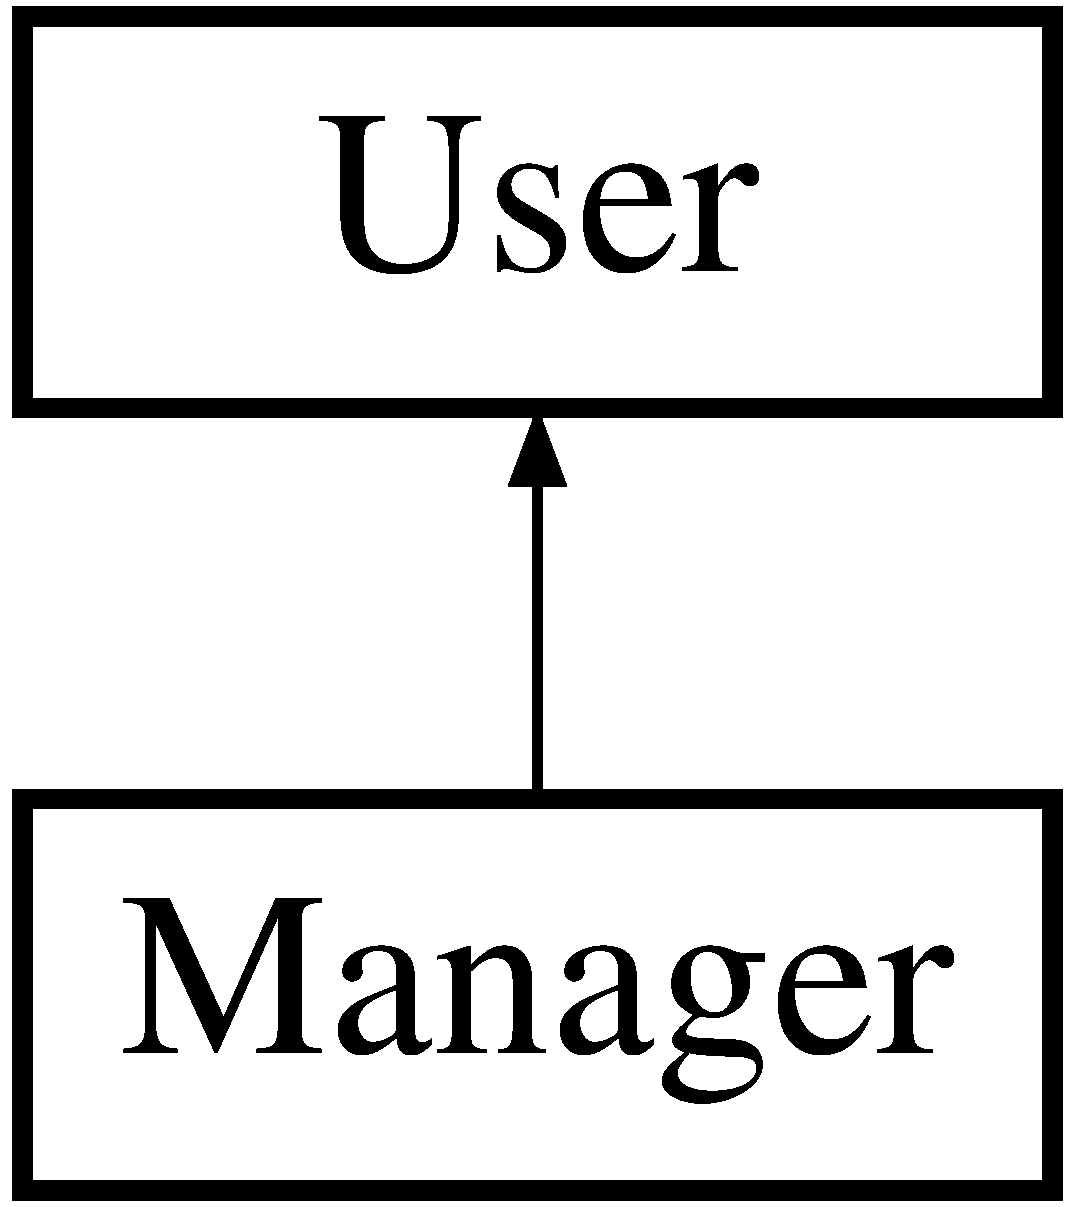
\includegraphics[height=2.000000cm]{classManager}
\end{center}
\end{figure}
\subsection*{Public Member Functions}
\begin{DoxyCompactItemize}
\item 
\hypertarget{classManager_ad2ee8089f5e80bc03fabcf9a493d045b}{{\bfseries Manager} (const \hyperlink{classUsrName}{Usr\-Name} \&, const \hyperlink{classUsrPassword}{Usr\-Password} \&, const \hyperlink{classUsrType}{Man\-Type} \&, const \hyperlink{classUsrMatric}{Usr\-Matric} \&)  throw (invalid\-\_\-argument)}\label{classManager_ad2ee8089f5e80bc03fabcf9a493d045b}

\item 
\hypertarget{classManager_a255ac6a7e2112631001296fa8db3811b}{\hyperlink{classUsrType}{Man\-Type} {\bfseries get\-Man\-Type} () const }\label{classManager_a255ac6a7e2112631001296fa8db3811b}

\item 
\hypertarget{classManager_a3d4e9cb6cc0e8d9be47fcc086b4e584e}{void {\bfseries set\-Man\-Type} (const \hyperlink{classUsrType}{Man\-Type} \&)}\label{classManager_a3d4e9cb6cc0e8d9be47fcc086b4e584e}

\item 
\hypertarget{classManager_a462f3704b016b57e087db417df73f07a}{\hyperlink{classUsrMatric}{Usr\-Matric} {\bfseries get\-Usr\-Matric} () const }\label{classManager_a462f3704b016b57e087db417df73f07a}

\item 
\hypertarget{classManager_a93309a0dde84dd0b5fe90d9e1da49822}{void {\bfseries set\-Usr\-Matric} (const \hyperlink{classUsrMatric}{Usr\-Matric} \&)}\label{classManager_a93309a0dde84dd0b5fe90d9e1da49822}

\end{DoxyCompactItemize}
\subsection*{Additional Inherited Members}


\subsection{Detailed Description}
Gerente; Onde ficarão armazenados os dados de usuários com privilégios administrativos sobre o sistema. 

Através desta classe é possível acessar o módulo de Usr\-Manage e modificar dados de outros usuários. 

The documentation for this class was generated from the following files\-:\begin{DoxyCompactItemize}
\item 
Entity\-Unit.\-h\item 
Entity\-Unit.\-cpp\end{DoxyCompactItemize}

\hypertarget{classMoney}{\section{Money Class Reference}
\label{classMoney}\index{Money@{Money}}
}


Define o limite da conta de um \hyperlink{classCustomer}{Customer} (Cliente).  




{\ttfamily \#include $<$Base\-Unit.\-h$>$}

Inheritance diagram for Money\-:\begin{figure}[H]
\begin{center}
\leavevmode
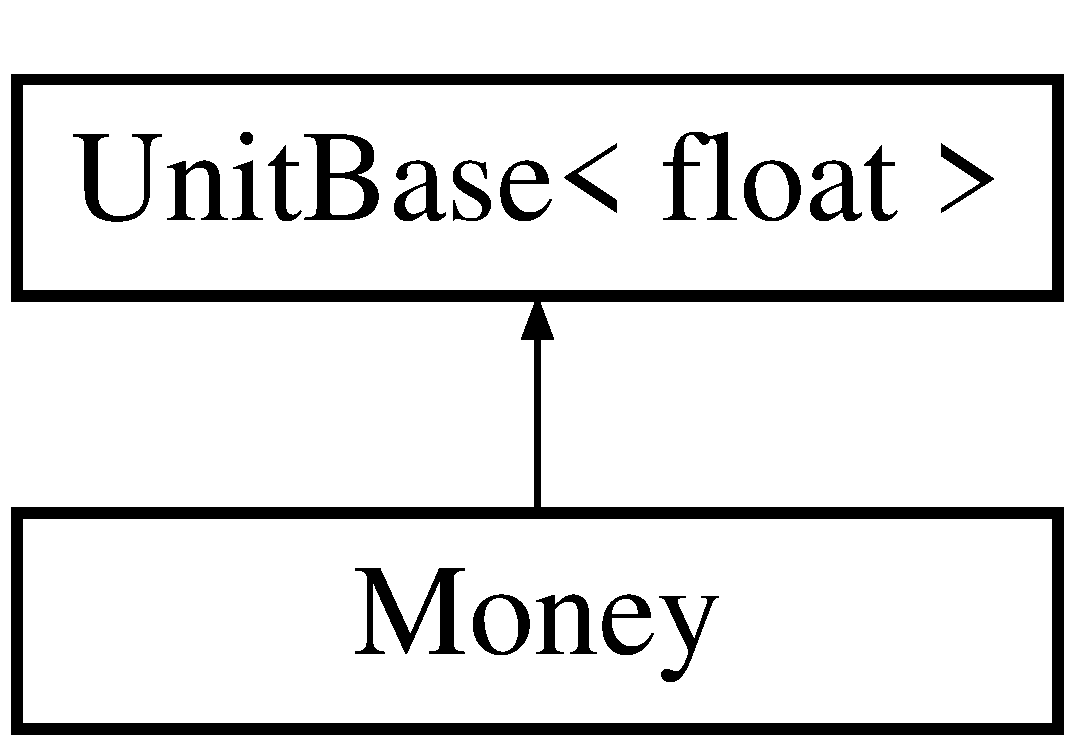
\includegraphics[height=2.000000cm]{classMoney}
\end{center}
\end{figure}
\subsection*{Public Member Functions}
\begin{DoxyCompactItemize}
\item 
\hypertarget{classMoney_a33986736e7432883ebd61584815b6681}{{\bfseries Money} (const float \&)  throw (invalid\-\_\-argument)}\label{classMoney_a33986736e7432883ebd61584815b6681}

\end{DoxyCompactItemize}
\subsection*{Additional Inherited Members}


\subsection{Detailed Description}
Define o limite da conta de um \hyperlink{classCustomer}{Customer} (Cliente). 

Atribui a cada conta um limite, limitando a utilização do crédito junto ao banco. 

The documentation for this class was generated from the following files\-:\begin{DoxyCompactItemize}
\item 
Base\-Unit.\-h\item 
Base\-Unit.\-cpp\end{DoxyCompactItemize}

\hypertarget{classPayCode}{\section{Pay\-Code Class Reference}
\label{classPayCode}\index{Pay\-Code@{Pay\-Code}}
}


Define um número de identificação para cada pagamento.  




{\ttfamily \#include $<$Base\-Unit.\-h$>$}

Inheritance diagram for Pay\-Code\-:\begin{figure}[H]
\begin{center}
\leavevmode
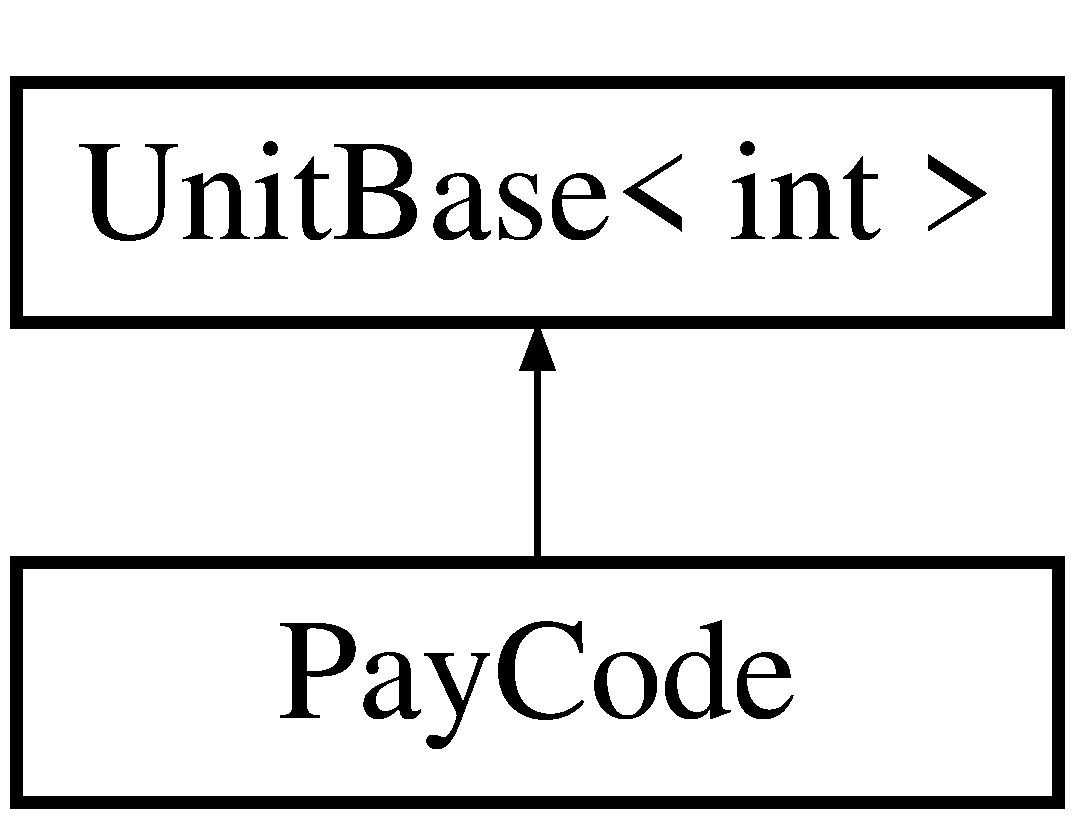
\includegraphics[height=2.000000cm]{classPayCode}
\end{center}
\end{figure}
\subsection*{Public Member Functions}
\begin{DoxyCompactItemize}
\item 
\hypertarget{classPayCode_a919ab6e420b9bd55e8c470ea411aa97e}{{\bfseries Pay\-Code} (const int \&)  throw (invalid\-\_\-argument)}\label{classPayCode_a919ab6e420b9bd55e8c470ea411aa97e}

\end{DoxyCompactItemize}
\subsection*{Additional Inherited Members}


\subsection{Detailed Description}
Define um número de identificação para cada pagamento. 

Atribui a cada pagamento um código, de forma a identificá-\/lo. 

The documentation for this class was generated from the following files\-:\begin{DoxyCompactItemize}
\item 
Base\-Unit.\-h\item 
Base\-Unit.\-cpp\end{DoxyCompactItemize}

\hypertarget{classPayDay}{\subsection{Pay\-Day Class Reference}
\label{dc/d17/classPayDay}\index{Pay\-Day@{Pay\-Day}}
}


Define a data do pagamento.  




{\ttfamily \#include $<$Base\-Unit.\-h$>$}

Inheritance diagram for Pay\-Day\-:\begin{figure}[H]
\begin{center}
\leavevmode
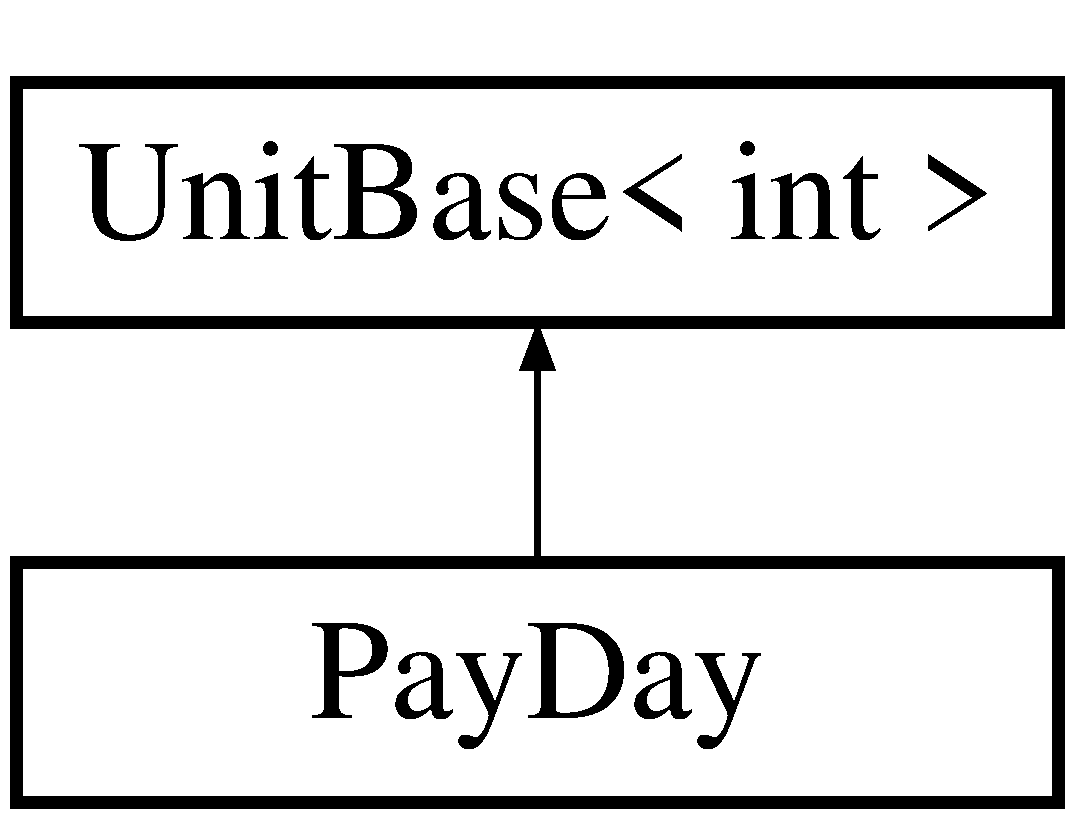
\includegraphics[height=2.000000cm]{dc/d17/classPayDay}
\end{center}
\end{figure}
\subsubsection*{Public Member Functions}
\begin{DoxyCompactItemize}
\item 
\hyperlink{classPayDay_a6da36cea0b2ac9a53106552aad00996a}{Pay\-Day} ()
\begin{DoxyCompactList}\small\item\em Construtor padrão de \hyperlink{classPayDay}{Pay\-Day}. \end{DoxyCompactList}\item 
\hyperlink{classPayDay_aa11abdfdb58bbd93f68bc02a7496e1c4}{Pay\-Day} (const int \&)  throw (invalid\-\_\-argument)
\begin{DoxyCompactList}\small\item\em Construtor base de \hyperlink{classPayDay}{Pay\-Day}. \end{DoxyCompactList}\item 
int \hyperlink{classPayDay_a297ce892f49aa9f3a504d514f171ed1d}{day} ()
\begin{DoxyCompactList}\small\item\em Método que retorna o dia contido na data. \end{DoxyCompactList}\item 
int \hyperlink{classPayDay_ada65e8834c142a95cd35ca2b399fbcde}{month} ()
\begin{DoxyCompactList}\small\item\em Método que retorna o mês contido na data. \end{DoxyCompactList}\item 
int \hyperlink{classPayDay_a962960925f9e6eaaac0fef5eb96849ec}{year} ()
\begin{DoxyCompactList}\small\item\em Método que retorna o ano contido na data. \end{DoxyCompactList}\end{DoxyCompactItemize}
\subsubsection*{Additional Inherited Members}


\subsubsection{Detailed Description}
Define a data do pagamento. 

Guarda a data de um pagamento num inteiro de formato D\-D\-M\-M\-A\-A\-A\-A. Dia, mês e ano devem ser acessados através dos atributos day, month, year. 

Definition at line 196 of file Base\-Unit.\-h.



\subsubsection{Constructor \& Destructor Documentation}
\hypertarget{classPayDay_a6da36cea0b2ac9a53106552aad00996a}{\index{Pay\-Day@{Pay\-Day}!Pay\-Day@{Pay\-Day}}
\index{Pay\-Day@{Pay\-Day}!PayDay@{Pay\-Day}}
\paragraph[{Pay\-Day}]{\setlength{\rightskip}{0pt plus 5cm}Pay\-Day\-::\-Pay\-Day (
\begin{DoxyParamCaption}
{}
\end{DoxyParamCaption}
)}}\label{dc/d17/classPayDay_a6da36cea0b2ac9a53106552aad00996a}


Construtor padrão de \hyperlink{classPayDay}{Pay\-Day}. 

Define o valor 0 como valor de não-\/inicialização deste tipo básico. 

Definition at line 173 of file Base\-Unit.\-cpp.

\hypertarget{classPayDay_aa11abdfdb58bbd93f68bc02a7496e1c4}{\index{Pay\-Day@{Pay\-Day}!Pay\-Day@{Pay\-Day}}
\index{Pay\-Day@{Pay\-Day}!PayDay@{Pay\-Day}}
\paragraph[{Pay\-Day}]{\setlength{\rightskip}{0pt plus 5cm}Pay\-Day\-::\-Pay\-Day (
\begin{DoxyParamCaption}
\item[{const int \&}]{date}
\end{DoxyParamCaption}
)  throw (invalid\-\_\-argument)}}\label{dc/d17/classPayDay_aa11abdfdb58bbd93f68bc02a7496e1c4}


Construtor base de \hyperlink{classPayDay}{Pay\-Day}. 

É preferível que se utilize este construtor pois ele já faz a validação automática do valor a ser definido. 

Definition at line 178 of file Base\-Unit.\-cpp.



\subsubsection{Member Function Documentation}
\hypertarget{classPayDay_a297ce892f49aa9f3a504d514f171ed1d}{\index{Pay\-Day@{Pay\-Day}!day@{day}}
\index{day@{day}!PayDay@{Pay\-Day}}
\paragraph[{day}]{\setlength{\rightskip}{0pt plus 5cm}int Pay\-Day\-::day (
\begin{DoxyParamCaption}
{}
\end{DoxyParamCaption}
)\hspace{0.3cm}{\ttfamily [inline]}}}\label{dc/d17/classPayDay_a297ce892f49aa9f3a504d514f171ed1d}


Método que retorna o dia contido na data. 

Extrai do inteiro contido no objeto o dia a que ele se refere. 

Definition at line 231 of file Base\-Unit.\-h.

\hypertarget{classPayDay_ada65e8834c142a95cd35ca2b399fbcde}{\index{Pay\-Day@{Pay\-Day}!month@{month}}
\index{month@{month}!PayDay@{Pay\-Day}}
\paragraph[{month}]{\setlength{\rightskip}{0pt plus 5cm}int Pay\-Day\-::month (
\begin{DoxyParamCaption}
{}
\end{DoxyParamCaption}
)\hspace{0.3cm}{\ttfamily [inline]}}}\label{dc/d17/classPayDay_ada65e8834c142a95cd35ca2b399fbcde}


Método que retorna o mês contido na data. 

Extrai do inteiro contido no objeto o mês a que ele se refere. 

Definition at line 226 of file Base\-Unit.\-h.

\hypertarget{classPayDay_a962960925f9e6eaaac0fef5eb96849ec}{\index{Pay\-Day@{Pay\-Day}!year@{year}}
\index{year@{year}!PayDay@{Pay\-Day}}
\paragraph[{year}]{\setlength{\rightskip}{0pt plus 5cm}int Pay\-Day\-::year (
\begin{DoxyParamCaption}
{}
\end{DoxyParamCaption}
)\hspace{0.3cm}{\ttfamily [inline]}}}\label{dc/d17/classPayDay_a962960925f9e6eaaac0fef5eb96849ec}


Método que retorna o ano contido na data. 

Extrai do inteiro contido no objeto o ano a que ele se refere. 

Definition at line 221 of file Base\-Unit.\-h.



The documentation for this class was generated from the following files\-:\begin{DoxyCompactItemize}
\item 
Base\-Unit.\-h\item 
Base\-Unit.\-cpp\end{DoxyCompactItemize}

\hypertarget{classPayment}{\section{Payment Class Reference}
\label{d5/d5e/classPayment}\index{Payment@{Payment}}
}


Pagamento; Onde ficarão armazenados dados sobre pagamentos a serem realizados.  




{\ttfamily \#include $<$Entity\-Unit.\-h$>$}

\subsection*{Public Member Functions}
\begin{DoxyCompactItemize}
\item 
\hyperlink{classPayment_a91b7742c5f9b4617e4a3bce6507cce49}{Payment} (const \hyperlink{classAccNumber}{Acc\-Number} \&, const \hyperlink{classPayDay}{Pay\-Day} \&, const \hyperlink{classMoney}{Money} \&)  throw (invalid\-\_\-argument)
\begin{DoxyCompactList}\small\item\em Construtor base de \hyperlink{classPayment}{Payment}. \end{DoxyCompactList}\item 
\hyperlink{classPayCode}{Pay\-Code} \hyperlink{classPayment_a1d71998fa33e757bb350eb40895865ae}{get\-Pay\-Code} () const 
\begin{DoxyCompactList}\small\item\em Método que recupera o valor contido no atributo pay\-Code. \end{DoxyCompactList}\item 
const \hyperlink{classPayCode}{Pay\-Code} \hyperlink{classPayment_adf458db6331e53948a473a04a0d622a4}{set\-Pay\-Code} (const \hyperlink{classPayCode}{Pay\-Code} \&)
\begin{DoxyCompactList}\small\item\em Método que define o valor no atributo pay\-Code. \end{DoxyCompactList}\item 
\hyperlink{classAccNumber}{Acc\-Number} \hyperlink{classPayment_a66c51330aef2e045884e25618a194904}{get\-Acc\-Number} () const 
\begin{DoxyCompactList}\small\item\em Método que recupera o valor contido no atributo acc\-Number. \end{DoxyCompactList}\item 
void \hyperlink{classPayment_a5d0e83f83f090acf4b33bc81f5391ca0}{set\-Acc\-Number} (const \hyperlink{classAccNumber}{Acc\-Number} \&)
\begin{DoxyCompactList}\small\item\em Método que define o valor no atributo pay\-Code. \end{DoxyCompactList}\item 
\hyperlink{classPayDay}{Pay\-Day} \hyperlink{classPayment_a22ee22d04f3f5757f115386aa3337c51}{get\-Pay\-Day} () const 
\begin{DoxyCompactList}\small\item\em Método que recupera o valor contido no atributo pay\-Day. \end{DoxyCompactList}\item 
void \hyperlink{classPayment_aaadd94e11ab24629d536809da691efc5}{set\-Pay\-Day} (const \hyperlink{classPayDay}{Pay\-Day} \&)
\begin{DoxyCompactList}\small\item\em Método que define o valor no atributo pay\-Code. \end{DoxyCompactList}\item 
\hyperlink{classMoney}{Money} \hyperlink{classPayment_a3a2d6a8dc3f6b63e924504e1994ae556}{get\-Pay\-Value} () const 
\begin{DoxyCompactList}\small\item\em Método que recupera o valor contido no atributo pay\-Value. \end{DoxyCompactList}\item 
void \hyperlink{classPayment_ace63ad77804d5a19ace50aa1a7335050}{set\-Pay\-Value} (const \hyperlink{classMoney}{Money} \&)
\begin{DoxyCompactList}\small\item\em Método que define o valor no atributo pay\-Code. \end{DoxyCompactList}\end{DoxyCompactItemize}


\subsection{Detailed Description}
Pagamento; Onde ficarão armazenados dados sobre pagamentos a serem realizados. 

Esta classe armazenará os dados de conta bem como a data agendada de pagamentos futuros. 

\subsection{Constructor \& Destructor Documentation}
\hypertarget{classPayment_a91b7742c5f9b4617e4a3bce6507cce49}{\index{Payment@{Payment}!Payment@{Payment}}
\index{Payment@{Payment}!Payment@{Payment}}
\subsubsection[{Payment}]{\setlength{\rightskip}{0pt plus 5cm}Payment\-::\-Payment (
\begin{DoxyParamCaption}
\item[{const {\bf Acc\-Number} \&}]{acc\-Number, }
\item[{const {\bf Pay\-Day} \&}]{pay\-Day, }
\item[{const {\bf Money} \&}]{pay\-Value}
\end{DoxyParamCaption}
)  throw (invalid\-\_\-argument)}}\label{d5/d5e/classPayment_a91b7742c5f9b4617e4a3bce6507cce49}


Construtor base de \hyperlink{classPayment}{Payment}. 

Define todos os atributos internos à classe automaticamente. 

\subsection{Member Function Documentation}
\hypertarget{classPayment_a66c51330aef2e045884e25618a194904}{\index{Payment@{Payment}!get\-Acc\-Number@{get\-Acc\-Number}}
\index{get\-Acc\-Number@{get\-Acc\-Number}!Payment@{Payment}}
\subsubsection[{get\-Acc\-Number}]{\setlength{\rightskip}{0pt plus 5cm}{\bf Acc\-Number} Payment\-::get\-Acc\-Number (
\begin{DoxyParamCaption}
{}
\end{DoxyParamCaption}
) const\hspace{0.3cm}{\ttfamily [inline]}}}\label{d5/d5e/classPayment_a66c51330aef2e045884e25618a194904}


Método que recupera o valor contido no atributo acc\-Number. 

O valor será retornado e o atributo não sofrerá nenhum tipo de alteração. \hypertarget{classPayment_a1d71998fa33e757bb350eb40895865ae}{\index{Payment@{Payment}!get\-Pay\-Code@{get\-Pay\-Code}}
\index{get\-Pay\-Code@{get\-Pay\-Code}!Payment@{Payment}}
\subsubsection[{get\-Pay\-Code}]{\setlength{\rightskip}{0pt plus 5cm}{\bf Pay\-Code} Payment\-::get\-Pay\-Code (
\begin{DoxyParamCaption}
{}
\end{DoxyParamCaption}
) const\hspace{0.3cm}{\ttfamily [inline]}}}\label{d5/d5e/classPayment_a1d71998fa33e757bb350eb40895865ae}


Método que recupera o valor contido no atributo pay\-Code. 

O valor será retornado e o atributo não sofrerá nenhum tipo de alteração. \hypertarget{classPayment_a22ee22d04f3f5757f115386aa3337c51}{\index{Payment@{Payment}!get\-Pay\-Day@{get\-Pay\-Day}}
\index{get\-Pay\-Day@{get\-Pay\-Day}!Payment@{Payment}}
\subsubsection[{get\-Pay\-Day}]{\setlength{\rightskip}{0pt plus 5cm}{\bf Pay\-Day} Payment\-::get\-Pay\-Day (
\begin{DoxyParamCaption}
{}
\end{DoxyParamCaption}
) const\hspace{0.3cm}{\ttfamily [inline]}}}\label{d5/d5e/classPayment_a22ee22d04f3f5757f115386aa3337c51}


Método que recupera o valor contido no atributo pay\-Day. 

O valor será retornado e o atributo não sofrerá nenhum tipo de alteração. \hypertarget{classPayment_a3a2d6a8dc3f6b63e924504e1994ae556}{\index{Payment@{Payment}!get\-Pay\-Value@{get\-Pay\-Value}}
\index{get\-Pay\-Value@{get\-Pay\-Value}!Payment@{Payment}}
\subsubsection[{get\-Pay\-Value}]{\setlength{\rightskip}{0pt plus 5cm}{\bf Money} Payment\-::get\-Pay\-Value (
\begin{DoxyParamCaption}
{}
\end{DoxyParamCaption}
) const}}\label{d5/d5e/classPayment_a3a2d6a8dc3f6b63e924504e1994ae556}


Método que recupera o valor contido no atributo pay\-Value. 

O valor será retornado e o atributo não sofrerá nenhum tipo de alteração. \hypertarget{classPayment_a5d0e83f83f090acf4b33bc81f5391ca0}{\index{Payment@{Payment}!set\-Acc\-Number@{set\-Acc\-Number}}
\index{set\-Acc\-Number@{set\-Acc\-Number}!Payment@{Payment}}
\subsubsection[{set\-Acc\-Number}]{\setlength{\rightskip}{0pt plus 5cm}void Payment\-::set\-Acc\-Number (
\begin{DoxyParamCaption}
\item[{const {\bf Acc\-Number} \&}]{acc\-Number}
\end{DoxyParamCaption}
)}}\label{d5/d5e/classPayment_a5d0e83f83f090acf4b33bc81f5391ca0}


Método que define o valor no atributo pay\-Code. 

\hypertarget{classPayment_adf458db6331e53948a473a04a0d622a4}{\index{Payment@{Payment}!set\-Pay\-Code@{set\-Pay\-Code}}
\index{set\-Pay\-Code@{set\-Pay\-Code}!Payment@{Payment}}
\subsubsection[{set\-Pay\-Code}]{\setlength{\rightskip}{0pt plus 5cm}const {\bf Pay\-Code} Payment\-::set\-Pay\-Code (
\begin{DoxyParamCaption}
\item[{const {\bf Pay\-Code} \&}]{}
\end{DoxyParamCaption}
)}}\label{d5/d5e/classPayment_adf458db6331e53948a473a04a0d622a4}


Método que define o valor no atributo pay\-Code. 

\hypertarget{classPayment_aaadd94e11ab24629d536809da691efc5}{\index{Payment@{Payment}!set\-Pay\-Day@{set\-Pay\-Day}}
\index{set\-Pay\-Day@{set\-Pay\-Day}!Payment@{Payment}}
\subsubsection[{set\-Pay\-Day}]{\setlength{\rightskip}{0pt plus 5cm}void Payment\-::set\-Pay\-Day (
\begin{DoxyParamCaption}
\item[{const {\bf Pay\-Day} \&}]{pay\-Day}
\end{DoxyParamCaption}
)}}\label{d5/d5e/classPayment_aaadd94e11ab24629d536809da691efc5}


Método que define o valor no atributo pay\-Code. 

\hypertarget{classPayment_ace63ad77804d5a19ace50aa1a7335050}{\index{Payment@{Payment}!set\-Pay\-Value@{set\-Pay\-Value}}
\index{set\-Pay\-Value@{set\-Pay\-Value}!Payment@{Payment}}
\subsubsection[{set\-Pay\-Value}]{\setlength{\rightskip}{0pt plus 5cm}void Payment\-::set\-Pay\-Value (
\begin{DoxyParamCaption}
\item[{const {\bf Money} \&}]{pay\-Value}
\end{DoxyParamCaption}
)}}\label{d5/d5e/classPayment_ace63ad77804d5a19ace50aa1a7335050}


Método que define o valor no atributo pay\-Code. 



The documentation for this class was generated from the following files\-:\begin{DoxyCompactItemize}
\item 
Entity\-Unit.\-h\item 
Entity\-Unit.\-cpp\end{DoxyCompactItemize}

\hypertarget{classPersBlkAccount}{\subsection{Pers\-Blk\-Account Class Reference}
\label{d6/d7d/classPersBlkAccount}\index{Pers\-Blk\-Account@{Pers\-Blk\-Account}}
}
Inheritance diagram for Pers\-Blk\-Account\-:\begin{figure}[H]
\begin{center}
\leavevmode
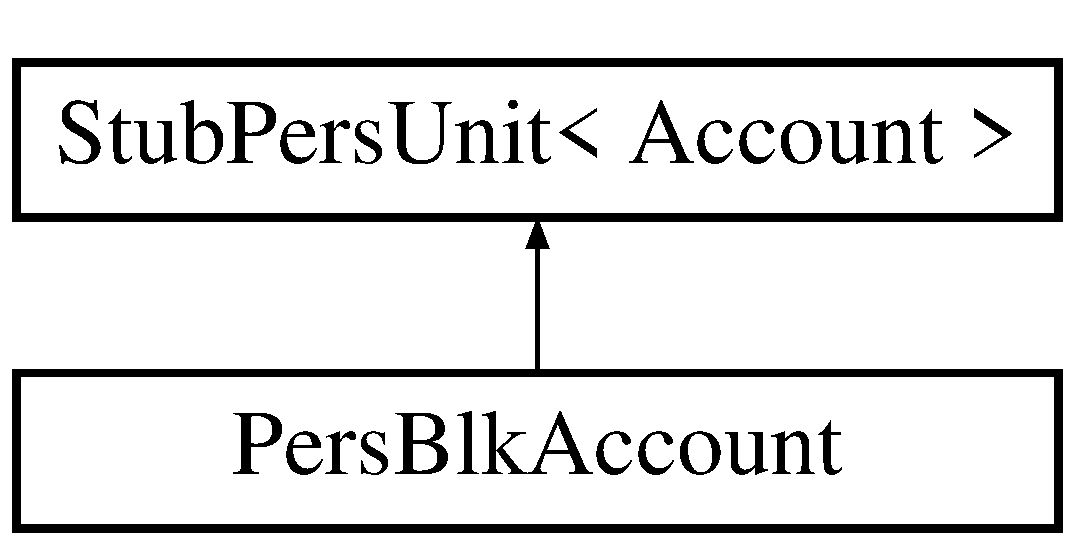
\includegraphics[height=2.000000cm]{d6/d7d/classPersBlkAccount}
\end{center}
\end{figure}
\subsubsection*{Public Member Functions}
\begin{DoxyCompactItemize}
\item 
\hypertarget{classPersBlkAccount_ac194c547436f62695c246d1f32e7574c}{void {\bfseries execute} (\hyperlink{classAccNumber}{Acc\-Number} $\ast$)  throw (\-Pers\-Error)}\label{d6/d7d/classPersBlkAccount_ac194c547436f62695c246d1f32e7574c}

\end{DoxyCompactItemize}
\subsubsection*{Additional Inherited Members}


\subsubsection{Detailed Description}


Definition at line 129 of file Pers\-Unit.\-h.



The documentation for this class was generated from the following files\-:\begin{DoxyCompactItemize}
\item 
Pers\-Unit.\-h\item 
Pers\-Unit.\-cpp\end{DoxyCompactItemize}

\hypertarget{classPersDelAccount}{\subsection{Pers\-Del\-Account Class Reference}
\label{d6/d74/classPersDelAccount}\index{Pers\-Del\-Account@{Pers\-Del\-Account}}
}
Inheritance diagram for Pers\-Del\-Account\-:\begin{figure}[H]
\begin{center}
\leavevmode
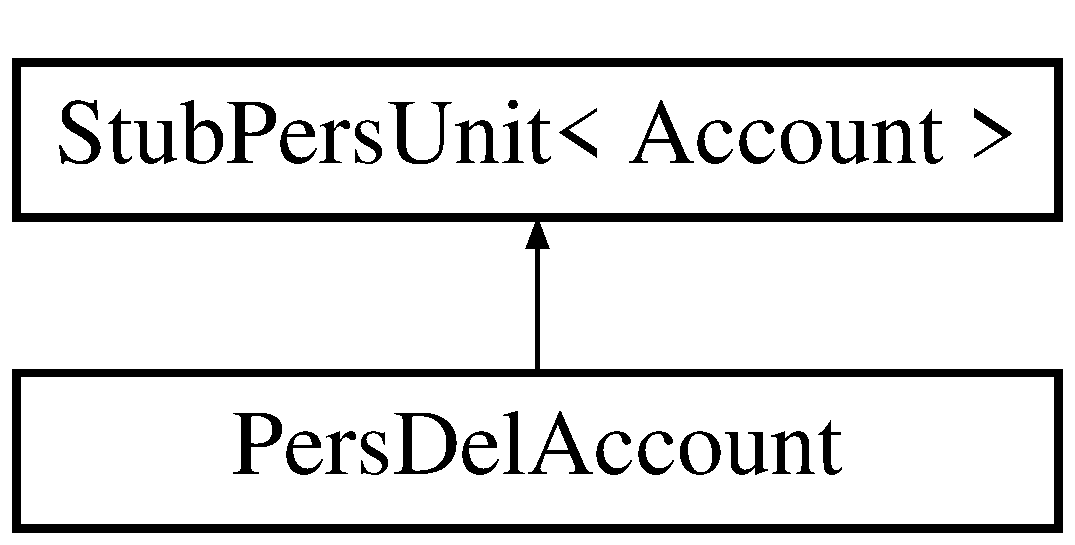
\includegraphics[height=2.000000cm]{d6/d74/classPersDelAccount}
\end{center}
\end{figure}
\subsubsection*{Public Member Functions}
\begin{DoxyCompactItemize}
\item 
\hypertarget{classPersDelAccount_a711d6dc413c1bc56ec70225ca6734c67}{void {\bfseries execute} (\hyperlink{classAccNumber}{Acc\-Number} $\ast$)  throw (\-Pers\-Error)}\label{d6/d74/classPersDelAccount_a711d6dc413c1bc56ec70225ca6734c67}

\end{DoxyCompactItemize}
\subsubsection*{Additional Inherited Members}


\subsubsection{Detailed Description}


Definition at line 117 of file Pers\-Unit.\-h.



The documentation for this class was generated from the following files\-:\begin{DoxyCompactItemize}
\item 
Pers\-Unit.\-h\item 
Pers\-Unit.\-cpp\end{DoxyCompactItemize}

\hypertarget{classPersDelManager}{\subsection{Pers\-Del\-Manager Class Reference}
\label{d6/d2b/classPersDelManager}\index{Pers\-Del\-Manager@{Pers\-Del\-Manager}}
}
Inheritance diagram for Pers\-Del\-Manager\-:\begin{figure}[H]
\begin{center}
\leavevmode
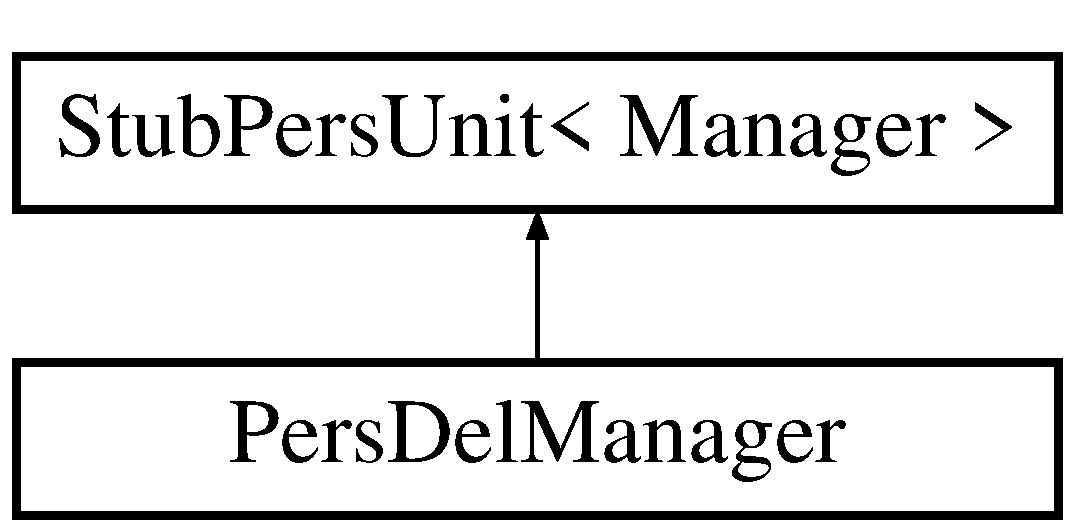
\includegraphics[height=2.000000cm]{d6/d2b/classPersDelManager}
\end{center}
\end{figure}
\subsubsection*{Public Member Functions}
\begin{DoxyCompactItemize}
\item 
\hypertarget{classPersDelManager_acd2f4ba61e71dee6f71fe8c5e37535a7}{void {\bfseries execute} (\hyperlink{classUsrMatric}{Usr\-Matric} $\ast$)  throw (\-Pers\-Error)}\label{d6/d2b/classPersDelManager_acd2f4ba61e71dee6f71fe8c5e37535a7}

\end{DoxyCompactItemize}
\subsubsection*{Additional Inherited Members}


\subsubsection{Detailed Description}


Definition at line 253 of file Pers\-Unit.\-h.



The documentation for this class was generated from the following files\-:\begin{DoxyCompactItemize}
\item 
Pers\-Unit.\-h\item 
Pers\-Unit.\-cpp\end{DoxyCompactItemize}

\hypertarget{classPersDelPayment}{\subsection{Pers\-Del\-Payment Class Reference}
\label{da/d8c/classPersDelPayment}\index{Pers\-Del\-Payment@{Pers\-Del\-Payment}}
}


Classe Command que deleta o registro de \hyperlink{classPayment}{Payment} relativo ao \hyperlink{classPayCode}{Pay\-Code} recebido.  




{\ttfamily \#include $<$Pers\-Unit.\-h$>$}

Inheritance diagram for Pers\-Del\-Payment\-:\begin{figure}[H]
\begin{center}
\leavevmode
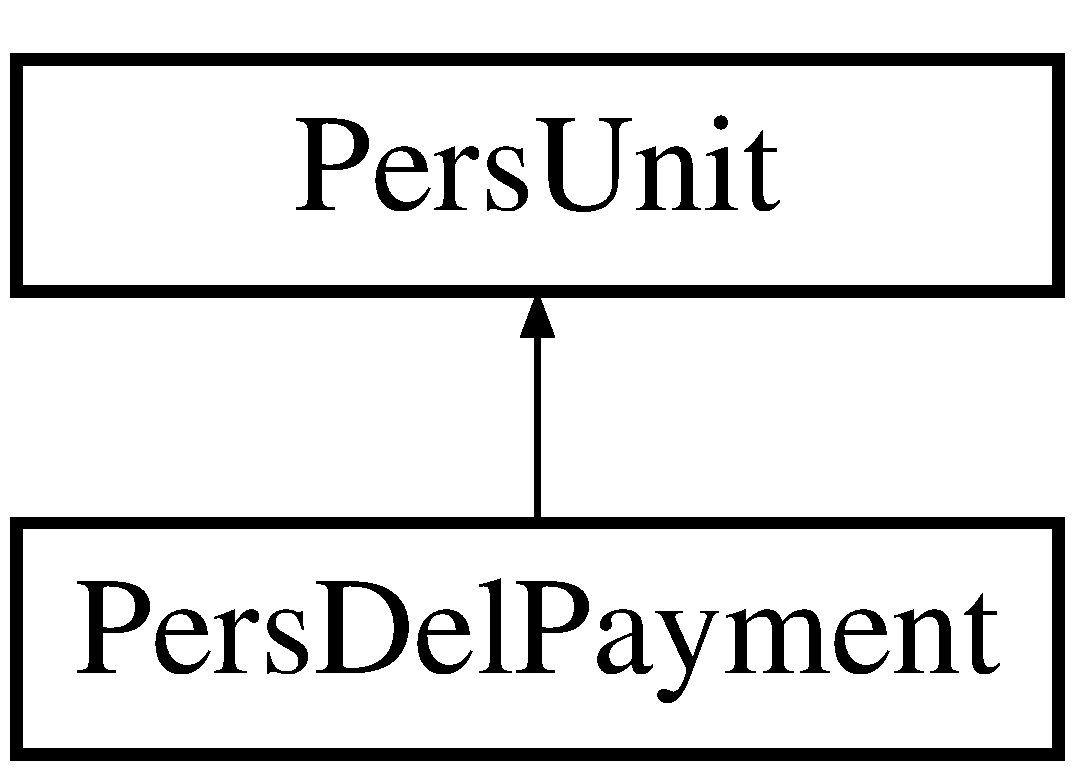
\includegraphics[height=2.000000cm]{da/d8c/classPersDelPayment}
\end{center}
\end{figure}
\subsubsection*{Public Member Functions}
\begin{DoxyCompactItemize}
\item 
\hypertarget{classPersDelPayment_a92f9a6d1cdca92afb3fa71a217026864}{void {\bfseries execute} (\hyperlink{classPayCode}{Pay\-Code} $\ast$)  throw (\-Pers\-Error)}\label{da/d8c/classPersDelPayment_a92f9a6d1cdca92afb3fa71a217026864}

\end{DoxyCompactItemize}
\subsubsection*{Additional Inherited Members}


\subsubsection{Detailed Description}
Classe Command que deleta o registro de \hyperlink{classPayment}{Payment} relativo ao \hyperlink{classPayCode}{Pay\-Code} recebido. 

Definition at line 152 of file Pers\-Unit.\-h.



The documentation for this class was generated from the following files\-:\begin{DoxyCompactItemize}
\item 
Pers\-Unit.\-h\item 
Pers\-Unit.\-cpp\end{DoxyCompactItemize}

\hypertarget{classPersEdtAccount}{\subsection{Pers\-Edt\-Account Class Reference}
\label{d9/d3d/classPersEdtAccount}\index{Pers\-Edt\-Account@{Pers\-Edt\-Account}}
}
Inheritance diagram for Pers\-Edt\-Account\-:\begin{figure}[H]
\begin{center}
\leavevmode
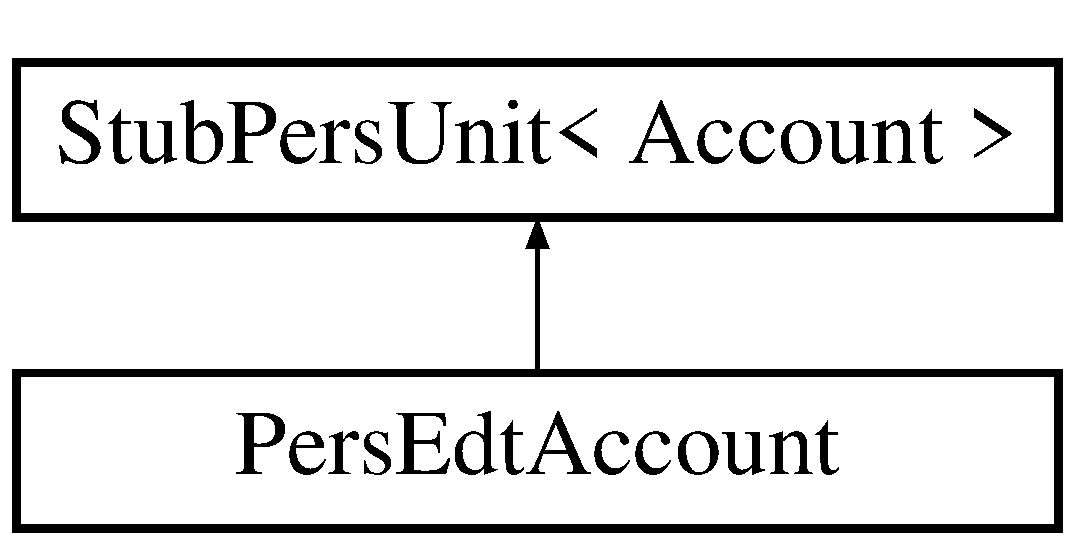
\includegraphics[height=2.000000cm]{d9/d3d/classPersEdtAccount}
\end{center}
\end{figure}
\subsubsection*{Public Member Functions}
\begin{DoxyCompactItemize}
\item 
\hypertarget{classPersEdtAccount_ad6ee8ffd77bd4e6e169c2cc1aca39619}{void {\bfseries execute} (\hyperlink{classAccNumber}{Acc\-Number} $\ast$, \hyperlink{classUsrType}{Acc\-Type} $\ast$)  throw (\-Pers\-Error)}\label{d9/d3d/classPersEdtAccount_ad6ee8ffd77bd4e6e169c2cc1aca39619}

\item 
\hypertarget{classPersEdtAccount_aacdc72e8ee1842be9516d0a17c043460}{void {\bfseries execute} (\hyperlink{classAccNumber}{Acc\-Number} $\ast$, \hyperlink{classMoney}{Money} $\ast$)  throw (\-Pers\-Error)}\label{d9/d3d/classPersEdtAccount_aacdc72e8ee1842be9516d0a17c043460}

\end{DoxyCompactItemize}
\subsubsection*{Additional Inherited Members}


\subsubsection{Detailed Description}


Definition at line 147 of file Pers\-Unit.\-h.



The documentation for this class was generated from the following files\-:\begin{DoxyCompactItemize}
\item 
Pers\-Unit.\-h\item 
Pers\-Unit.\-cpp\end{DoxyCompactItemize}

\hypertarget{classPersEdtCustomer}{\subsection{Pers\-Edt\-Customer Class Reference}
\label{de/d6a/classPersEdtCustomer}\index{Pers\-Edt\-Customer@{Pers\-Edt\-Customer}}
}
Inheritance diagram for Pers\-Edt\-Customer\-:\begin{figure}[H]
\begin{center}
\leavevmode
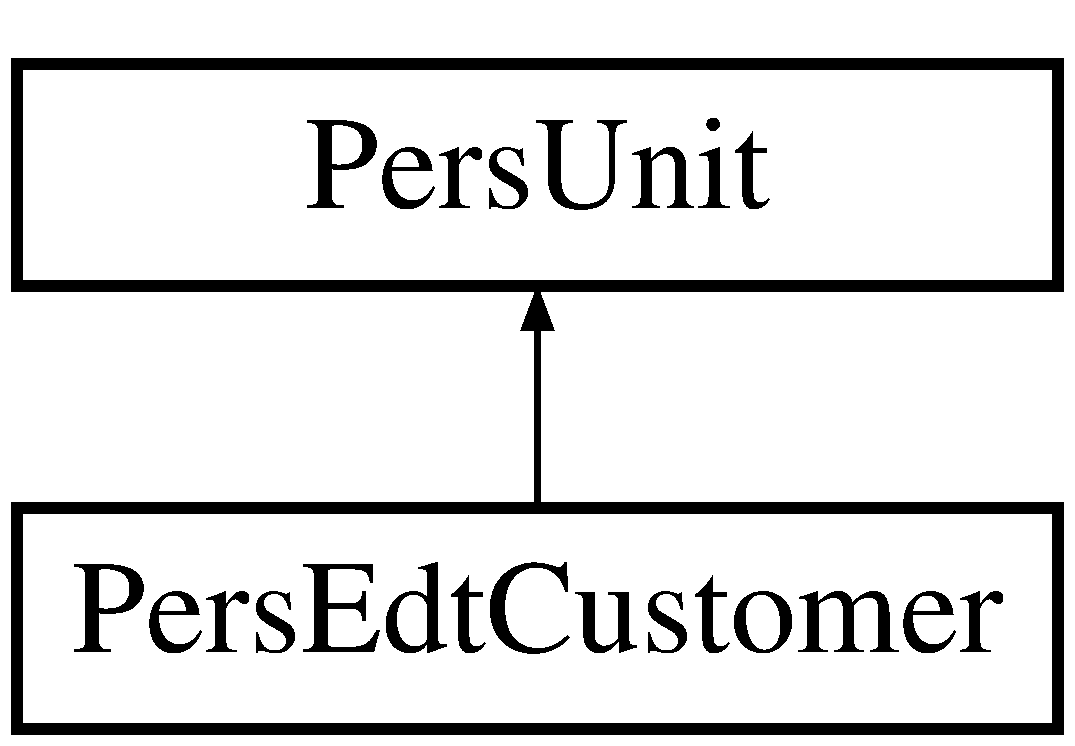
\includegraphics[height=2.000000cm]{de/d6a/classPersEdtCustomer}
\end{center}
\end{figure}
\subsubsection*{Public Member Functions}
\begin{DoxyCompactItemize}
\item 
\hypertarget{classPersEdtCustomer_a5275d925c901c95fbeb2036cd5c8e91e}{void {\bfseries execute} (\hyperlink{classUsrId}{Usr\-Id} $\ast$, \hyperlink{classUsrName}{Usr\-Name} $\ast$)  throw (\-Pers\-Error)}\label{de/d6a/classPersEdtCustomer_a5275d925c901c95fbeb2036cd5c8e91e}

\item 
\hypertarget{classPersEdtCustomer_a317d8e46e20e7bf342125dc6fda3adb9}{void {\bfseries execute} (\hyperlink{classUsrId}{Usr\-Id} \&, \hyperlink{classUsrPassword}{Usr\-Password} \&)  throw (\-Pers\-Error)}\label{de/d6a/classPersEdtCustomer_a317d8e46e20e7bf342125dc6fda3adb9}

\end{DoxyCompactItemize}
\subsubsection*{Additional Inherited Members}


\subsubsection{Detailed Description}


Definition at line 198 of file Pers\-Unit.\-h.



The documentation for this class was generated from the following files\-:\begin{DoxyCompactItemize}
\item 
Pers\-Unit.\-h\item 
Pers\-Unit.\-cpp\end{DoxyCompactItemize}

\hypertarget{classPersEdtManager}{\subsection{Pers\-Edt\-Manager Class Reference}
\label{da/dab/classPersEdtManager}\index{Pers\-Edt\-Manager@{Pers\-Edt\-Manager}}
}
Inheritance diagram for Pers\-Edt\-Manager\-:\begin{figure}[H]
\begin{center}
\leavevmode
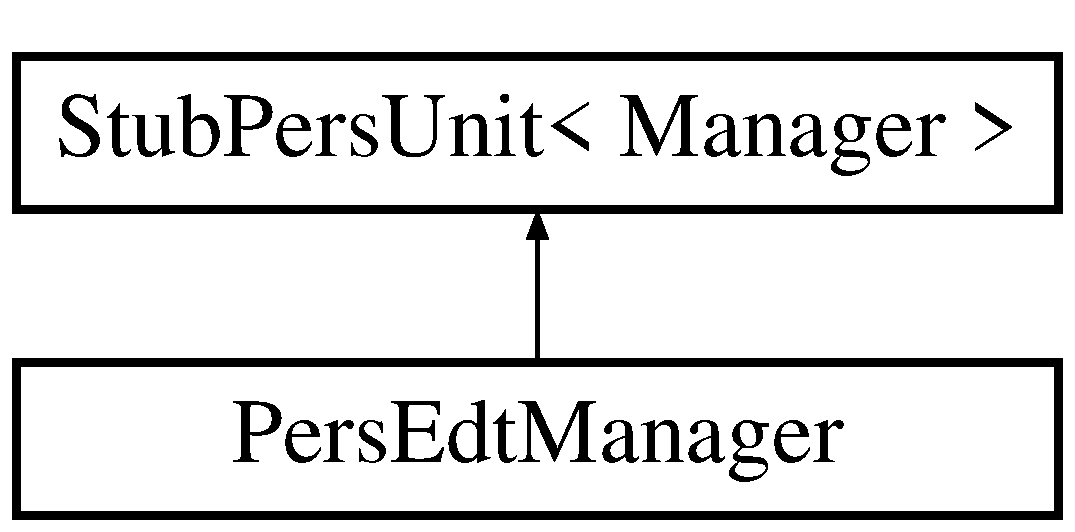
\includegraphics[height=2.000000cm]{da/dab/classPersEdtManager}
\end{center}
\end{figure}
\subsubsection*{Public Member Functions}
\begin{DoxyCompactItemize}
\item 
\hypertarget{classPersEdtManager_a537ffad367877114dc9c159fd1eb346e}{void {\bfseries execute} (\hyperlink{classUsrMatric}{Usr\-Matric} $\ast$, \hyperlink{classUsrName}{Usr\-Name} $\ast$)  throw (\-Pers\-Error)}\label{da/dab/classPersEdtManager_a537ffad367877114dc9c159fd1eb346e}

\item 
\hypertarget{classPersEdtManager_a7fa79580f771a5798e819a55ae5fb815}{void {\bfseries execute} (\hyperlink{classUsrMatric}{Usr\-Matric} $\ast$, \hyperlink{classUsrPassword}{Usr\-Password} $\ast$)  throw (\-Pers\-Error)}\label{da/dab/classPersEdtManager_a7fa79580f771a5798e819a55ae5fb815}

\end{DoxyCompactItemize}
\subsubsection*{Additional Inherited Members}


\subsubsection{Detailed Description}


Definition at line 166 of file Pers\-Unit.\-h.



The documentation for this class was generated from the following files\-:\begin{DoxyCompactItemize}
\item 
Pers\-Unit.\-h\item 
Pers\-Unit.\-cpp\end{DoxyCompactItemize}

\hypertarget{classPersError}{\section{Pers\-Error Class Reference}
\label{da/dcf/classPersError}\index{Pers\-Error@{Pers\-Error}}
}
\subsection*{Public Member Functions}
\begin{DoxyCompactItemize}
\item 
\hypertarget{classPersError_a6c7a979c6ac884b820657e54331d68a6}{{\bfseries Pers\-Error} (string)}\label{da/dcf/classPersError_a6c7a979c6ac884b820657e54331d68a6}

\item 
\hypertarget{classPersError_a92a1000d4105875297edcefb5a78b77c}{string {\bfseries what} ()}\label{da/dcf/classPersError_a92a1000d4105875297edcefb5a78b77c}

\end{DoxyCompactItemize}


The documentation for this class was generated from the following files\-:\begin{DoxyCompactItemize}
\item 
Pers\-Unit.\-h\item 
Pers\-Unit.\-cpp\end{DoxyCompactItemize}

\hypertarget{classPersFetchAccount}{\subsection{Pers\-Fetch\-Account Class Reference}
\label{df/d2b/classPersFetchAccount}\index{Pers\-Fetch\-Account@{Pers\-Fetch\-Account}}
}
Inheritance diagram for Pers\-Fetch\-Account\-:\begin{figure}[H]
\begin{center}
\leavevmode
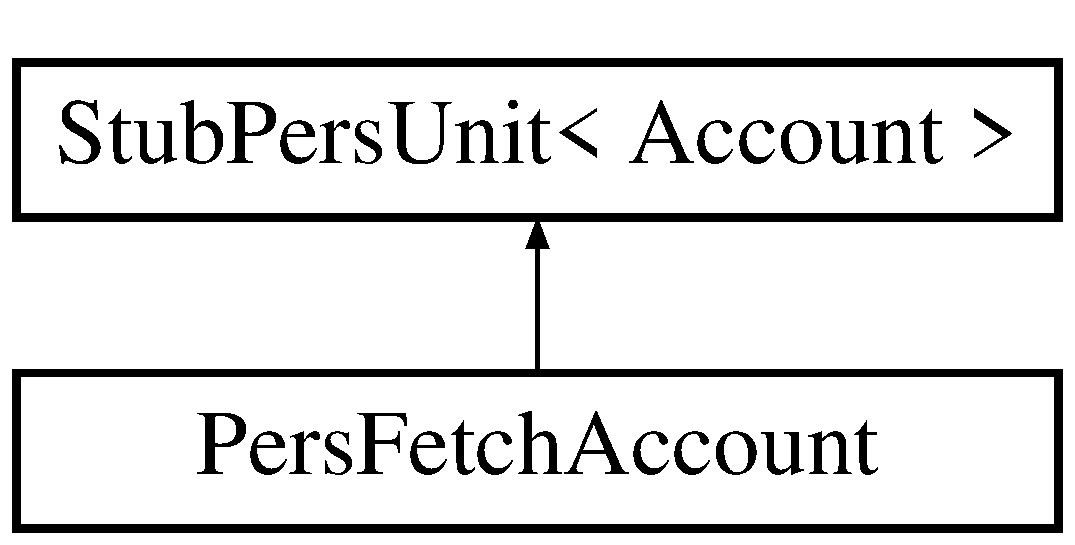
\includegraphics[height=2.000000cm]{df/d2b/classPersFetchAccount}
\end{center}
\end{figure}
\subsubsection*{Public Member Functions}
\begin{DoxyCompactItemize}
\item 
\hypertarget{classPersFetchAccount_a8fb6e7e8a65bebe14be61fb1a3c7f471}{void {\bfseries execute} ()  throw (\-Pers\-Error)}\label{df/d2b/classPersFetchAccount_a8fb6e7e8a65bebe14be61fb1a3c7f471}

\end{DoxyCompactItemize}
\subsubsection*{Additional Inherited Members}


\subsubsection{Detailed Description}


Definition at line 135 of file Pers\-Unit.\-h.



The documentation for this class was generated from the following files\-:\begin{DoxyCompactItemize}
\item 
Pers\-Unit.\-h\item 
Pers\-Unit.\-cpp\end{DoxyCompactItemize}

\hypertarget{classPersFetchManager}{\subsection{Pers\-Fetch\-Manager Class Reference}
\label{d7/de3/classPersFetchManager}\index{Pers\-Fetch\-Manager@{Pers\-Fetch\-Manager}}
}
Inheritance diagram for Pers\-Fetch\-Manager\-:\begin{figure}[H]
\begin{center}
\leavevmode
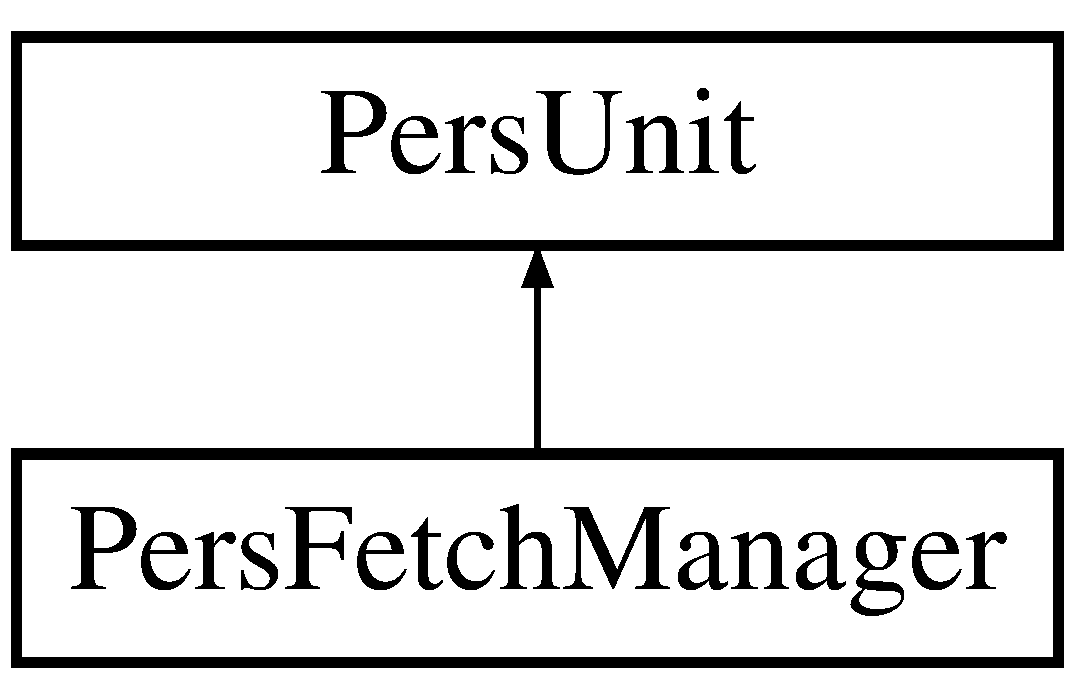
\includegraphics[height=2.000000cm]{d7/de3/classPersFetchManager}
\end{center}
\end{figure}
\subsubsection*{Public Member Functions}
\begin{DoxyCompactItemize}
\item 
\hypertarget{classPersFetchManager_aca78de204167406eb461f932e05d6920}{void {\bfseries execute} ()  throw (\-Pers\-Error)}\label{d7/de3/classPersFetchManager_aca78de204167406eb461f932e05d6920}

\end{DoxyCompactItemize}
\subsubsection*{Additional Inherited Members}


\subsubsection{Detailed Description}


Definition at line 160 of file Pers\-Unit.\-h.



The documentation for this class was generated from the following files\-:\begin{DoxyCompactItemize}
\item 
Pers\-Unit.\-h\item 
Pers\-Unit.\-cpp\end{DoxyCompactItemize}

\hypertarget{classPersFetchPayment}{\subsection{Pers\-Fetch\-Payment Class Reference}
\label{d6/d08/classPersFetchPayment}\index{Pers\-Fetch\-Payment@{Pers\-Fetch\-Payment}}
}


Classe Command que retorna uma lista de pagamentos cadastrados no banco de dados.  




{\ttfamily \#include $<$Pers\-Unit.\-h$>$}

Inheritance diagram for Pers\-Fetch\-Payment\-:\begin{figure}[H]
\begin{center}
\leavevmode
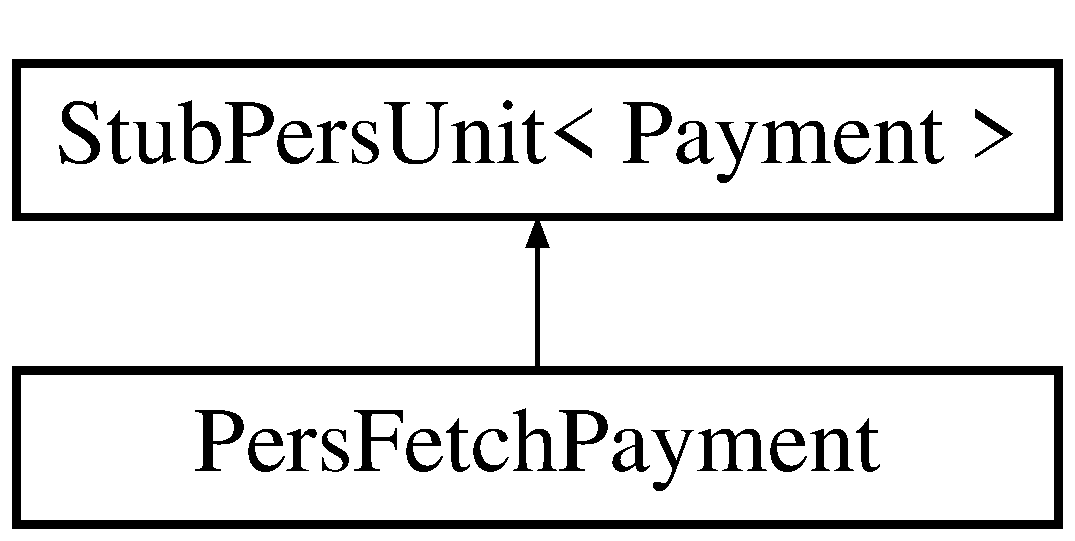
\includegraphics[height=2.000000cm]{d6/d08/classPersFetchPayment}
\end{center}
\end{figure}
\subsubsection*{Public Member Functions}
\begin{DoxyCompactItemize}
\item 
\hypertarget{classPersFetchPayment_a5d2e631be69299b14ee9634cb5fbf56f}{void {\bfseries execute} ()  throw (\-Pers\-Error)}\label{d6/d08/classPersFetchPayment_a5d2e631be69299b14ee9634cb5fbf56f}

\item 
\hypertarget{classPersFetchPayment_a238f366d821711dd7aba421c1a581c0a}{list$<$ \hyperlink{classPayment}{Payment} $>$ {\bfseries get\-Result} ()}\label{d6/d08/classPersFetchPayment_a238f366d821711dd7aba421c1a581c0a}

\end{DoxyCompactItemize}
\subsubsection*{Additional Inherited Members}


\subsubsection{Detailed Description}
Classe Command que retorna uma lista de pagamentos cadastrados no banco de dados. 

Definition at line 159 of file Pers\-Unit.\-h.



The documentation for this class was generated from the following files\-:\begin{DoxyCompactItemize}
\item 
Pers\-Unit.\-h\item 
Pers\-Unit.\-cpp\end{DoxyCompactItemize}

\hypertarget{classPersGetAccount}{\subsection{Pers\-Get\-Account Class Reference}
\label{d1/d40/classPersGetAccount}\index{Pers\-Get\-Account@{Pers\-Get\-Account}}
}
Inheritance diagram for Pers\-Get\-Account\-:\begin{figure}[H]
\begin{center}
\leavevmode
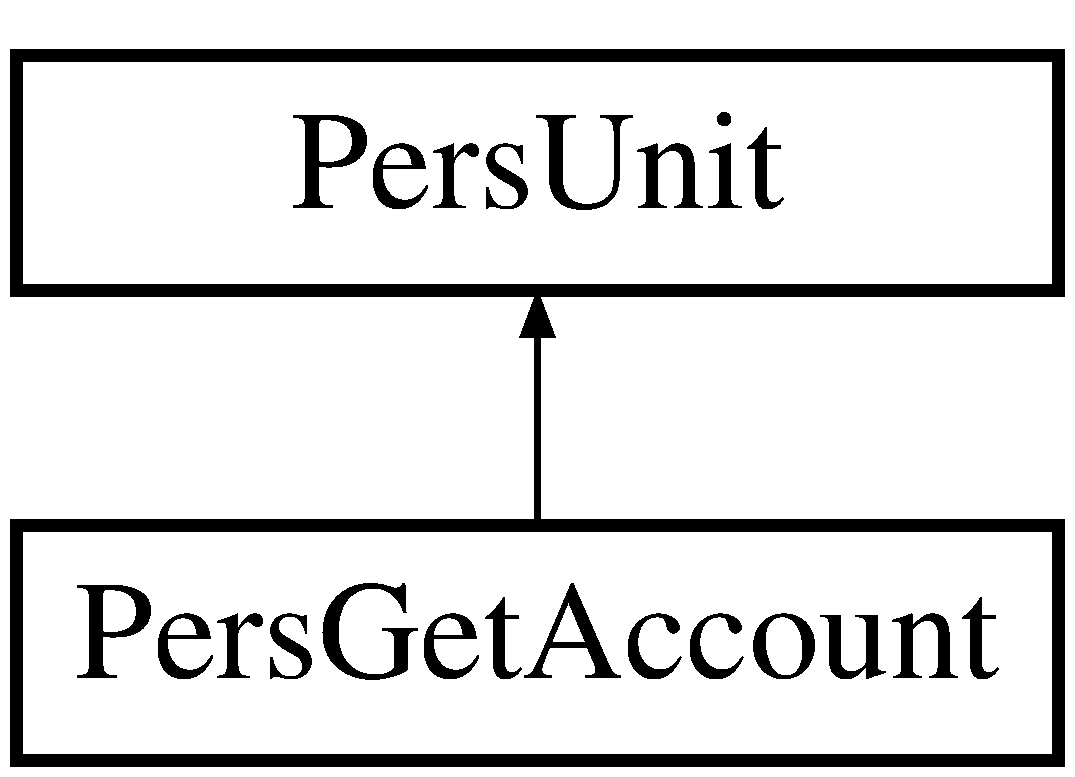
\includegraphics[height=2.000000cm]{d1/d40/classPersGetAccount}
\end{center}
\end{figure}
\subsubsection*{Public Member Functions}
\begin{DoxyCompactItemize}
\item 
\hypertarget{classPersGetAccount_aebcae427483ef6221ca67c07469d7182}{void {\bfseries execute} (\hyperlink{classAccNumber}{Acc\-Number} $\ast$)  throw (\-Pers\-Error)}\label{d1/d40/classPersGetAccount_aebcae427483ef6221ca67c07469d7182}

\end{DoxyCompactItemize}
\subsubsection*{Additional Inherited Members}


\subsubsection{Detailed Description}


Definition at line 99 of file Pers\-Unit.\-h.



The documentation for this class was generated from the following files\-:\begin{DoxyCompactItemize}
\item 
Pers\-Unit.\-h\item 
Pers\-Unit.\-cpp\end{DoxyCompactItemize}

\hypertarget{classPersGetBalance}{\subsection{Pers\-Get\-Balance Class Reference}
\label{d3/d71/classPersGetBalance}\index{Pers\-Get\-Balance@{Pers\-Get\-Balance}}
}


Classe Command que retorna o Balance de uma conta de número \hyperlink{classAccNumber}{Acc\-Number}.  




{\ttfamily \#include $<$Pers\-Unit.\-h$>$}

Inheritance diagram for Pers\-Get\-Balance\-:\begin{figure}[H]
\begin{center}
\leavevmode
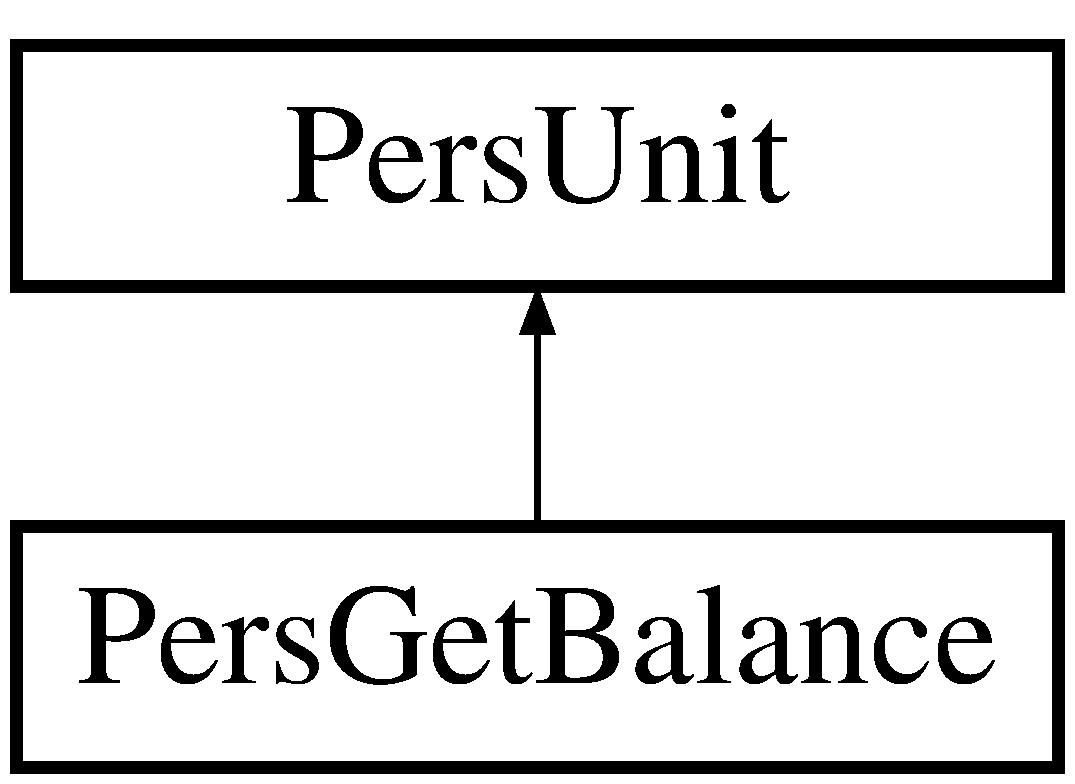
\includegraphics[height=2.000000cm]{d3/d71/classPersGetBalance}
\end{center}
\end{figure}
\subsubsection*{Public Member Functions}
\begin{DoxyCompactItemize}
\item 
\hypertarget{classPersGetBalance_a265f69b7d01b99c252f421eec95dcedb}{void {\bfseries execute} (\hyperlink{classAccNumber}{Acc\-Number})  throw (\-Pers\-Error, invalid\-\_\-argument)}\label{d3/d71/classPersGetBalance_a265f69b7d01b99c252f421eec95dcedb}

\item 
\hypertarget{classPersGetBalance_a4df3579dbede5f9c38d25c1b937c88e7}{\hyperlink{classMoney}{Money} {\bfseries get\-Result} ()}\label{d3/d71/classPersGetBalance_a4df3579dbede5f9c38d25c1b937c88e7}

\end{DoxyCompactItemize}
\subsubsection*{Additional Inherited Members}


\subsubsection{Detailed Description}
Classe Command que retorna o Balance de uma conta de número \hyperlink{classAccNumber}{Acc\-Number}. 

Definition at line 122 of file Pers\-Unit.\-h.



The documentation for this class was generated from the following files\-:\begin{DoxyCompactItemize}
\item 
Pers\-Unit.\-h\item 
Pers\-Unit.\-cpp\end{DoxyCompactItemize}

\hypertarget{classPersGetCustomer}{\subsection{Pers\-Get\-Customer Class Reference}
\label{df/dac/classPersGetCustomer}\index{Pers\-Get\-Customer@{Pers\-Get\-Customer}}
}
Inheritance diagram for Pers\-Get\-Customer\-:\begin{figure}[H]
\begin{center}
\leavevmode
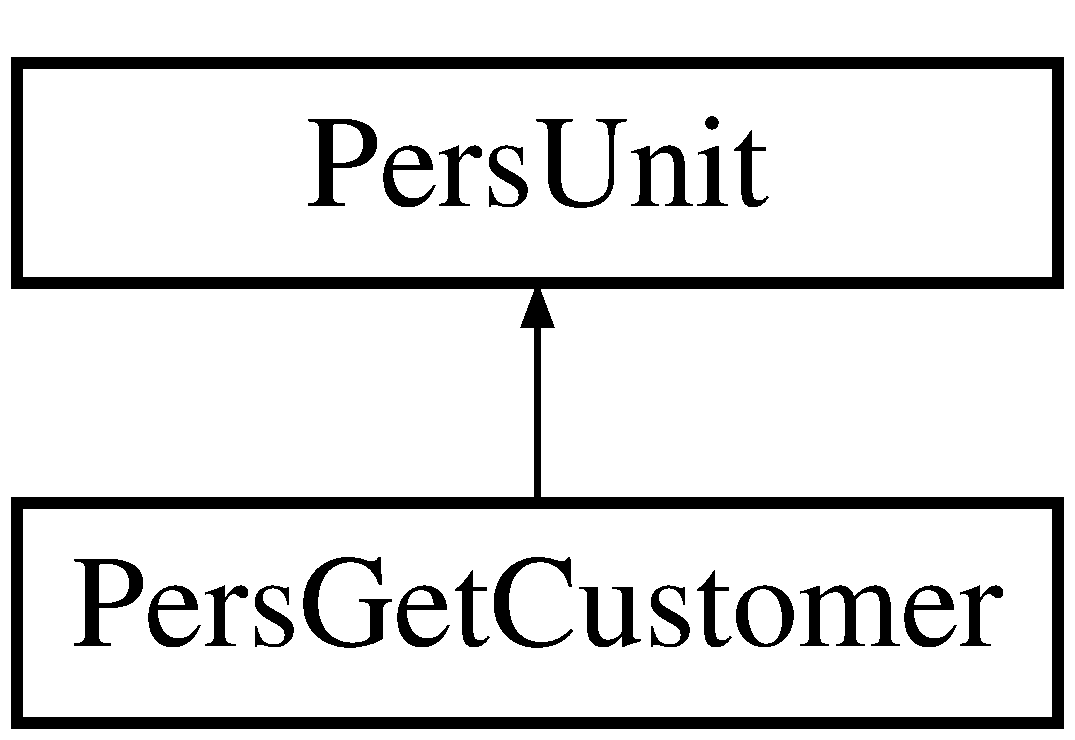
\includegraphics[height=2.000000cm]{df/dac/classPersGetCustomer}
\end{center}
\end{figure}
\subsubsection*{Public Member Functions}
\begin{DoxyCompactItemize}
\item 
\hypertarget{classPersGetCustomer_a67103ecb49882a8287849fa649cc9047}{void {\bfseries execute} (\hyperlink{classUsrId}{Usr\-Id})  throw (\-Pers\-Error)}\label{df/dac/classPersGetCustomer_a67103ecb49882a8287849fa649cc9047}

\item 
\hypertarget{classPersGetCustomer_a8d72d5fab3bc9c78b1e4af33e535b89f}{void {\bfseries execute} (\hyperlink{classUsrName}{Usr\-Name} $\ast$)  throw (\-Pers\-Error)}\label{df/dac/classPersGetCustomer_a8d72d5fab3bc9c78b1e4af33e535b89f}

\end{DoxyCompactItemize}
\subsubsection*{Additional Inherited Members}


\subsubsection{Detailed Description}


Definition at line 179 of file Pers\-Unit.\-h.



The documentation for this class was generated from the following files\-:\begin{DoxyCompactItemize}
\item 
Pers\-Unit.\-h\item 
Pers\-Unit.\-cpp\end{DoxyCompactItemize}

\hypertarget{classPersGetLatestCode}{\subsection{Pers\-Get\-Latest\-Code Class Reference}
\label{d8/d77/classPersGetLatestCode}\index{Pers\-Get\-Latest\-Code@{Pers\-Get\-Latest\-Code}}
}


Classe Command que retorna o menor \hyperlink{classPayCode}{Pay\-Code} disponível para criação de contas.  




{\ttfamily \#include $<$Pers\-Unit.\-h$>$}

Inheritance diagram for Pers\-Get\-Latest\-Code\-:\begin{figure}[H]
\begin{center}
\leavevmode
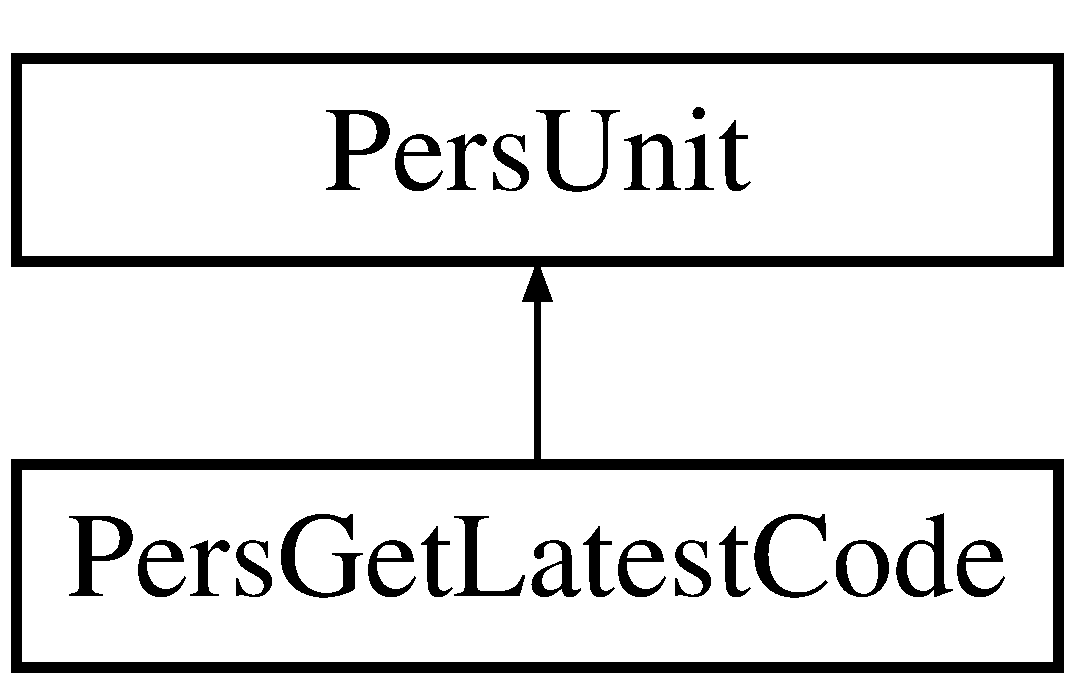
\includegraphics[height=2.000000cm]{d8/d77/classPersGetLatestCode}
\end{center}
\end{figure}
\subsubsection*{Public Member Functions}
\begin{DoxyCompactItemize}
\item 
\hypertarget{classPersGetLatestCode_ad053433ea59b9c3caa4b1baf702add8f}{void {\bfseries execute} ()  throw (\-Pers\-Error)}\label{d8/d77/classPersGetLatestCode_ad053433ea59b9c3caa4b1baf702add8f}

\item 
\hypertarget{classPersGetLatestCode_aa036c4249daec1f19e63c1411f8bd988}{\hyperlink{classPayCode}{Pay\-Code} {\bfseries get\-Result} ()}\label{d8/d77/classPersGetLatestCode_aa036c4249daec1f19e63c1411f8bd988}

\end{DoxyCompactItemize}
\subsubsection*{Additional Inherited Members}


\subsubsection{Detailed Description}
Classe Command que retorna o menor \hyperlink{classPayCode}{Pay\-Code} disponível para criação de contas. 

Definition at line 137 of file Pers\-Unit.\-h.



The documentation for this class was generated from the following files\-:\begin{DoxyCompactItemize}
\item 
Pers\-Unit.\-h\item 
Pers\-Unit.\-cpp\end{DoxyCompactItemize}

\hypertarget{classPersGetLatestId}{\subsection{Pers\-Get\-Latest\-Id Class Reference}
\label{d3/dab/classPersGetLatestId}\index{Pers\-Get\-Latest\-Id@{Pers\-Get\-Latest\-Id}}
}
Inheritance diagram for Pers\-Get\-Latest\-Id\-:\begin{figure}[H]
\begin{center}
\leavevmode
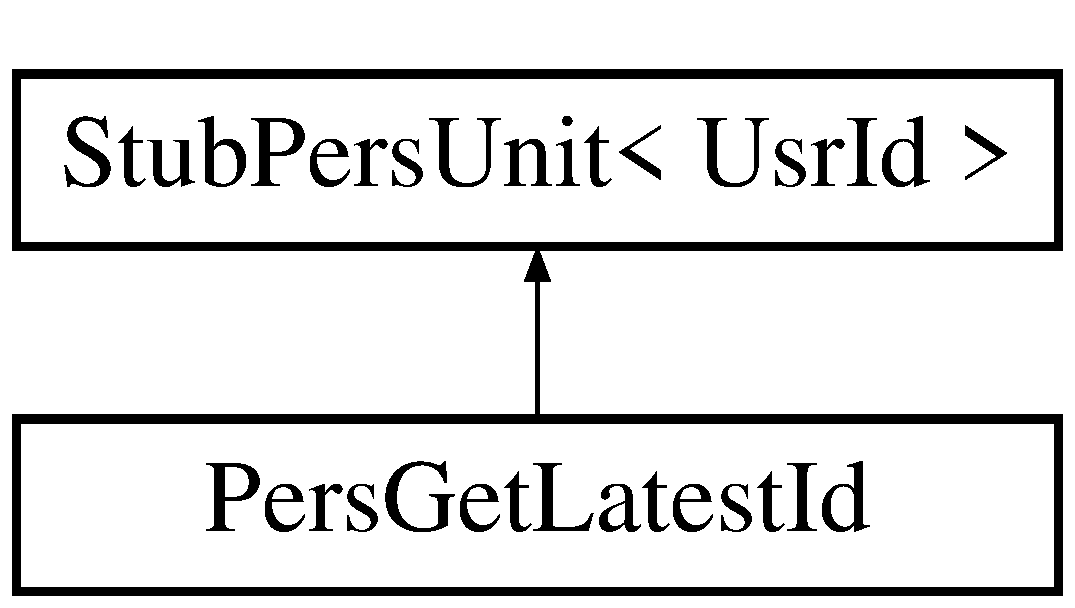
\includegraphics[height=2.000000cm]{d3/dab/classPersGetLatestId}
\end{center}
\end{figure}
\subsubsection*{Public Member Functions}
\begin{DoxyCompactItemize}
\item 
\hypertarget{classPersGetLatestId_a11340d0091a1d8bf164011be400609f7}{void {\bfseries execute} ()  throw (\-Pers\-Error)}\label{d3/dab/classPersGetLatestId_a11340d0091a1d8bf164011be400609f7}

\end{DoxyCompactItemize}
\subsubsection*{Additional Inherited Members}


\subsubsection{Detailed Description}


Definition at line 192 of file Pers\-Unit.\-h.



The documentation for this class was generated from the following files\-:\begin{DoxyCompactItemize}
\item 
Pers\-Unit.\-h\item 
Pers\-Unit.\-cpp\end{DoxyCompactItemize}

\hypertarget{classPersGetLatestMatric}{\subsection{Pers\-Get\-Latest\-Matric Class Reference}
\label{de/d05/classPersGetLatestMatric}\index{Pers\-Get\-Latest\-Matric@{Pers\-Get\-Latest\-Matric}}
}
Inheritance diagram for Pers\-Get\-Latest\-Matric\-:\begin{figure}[H]
\begin{center}
\leavevmode
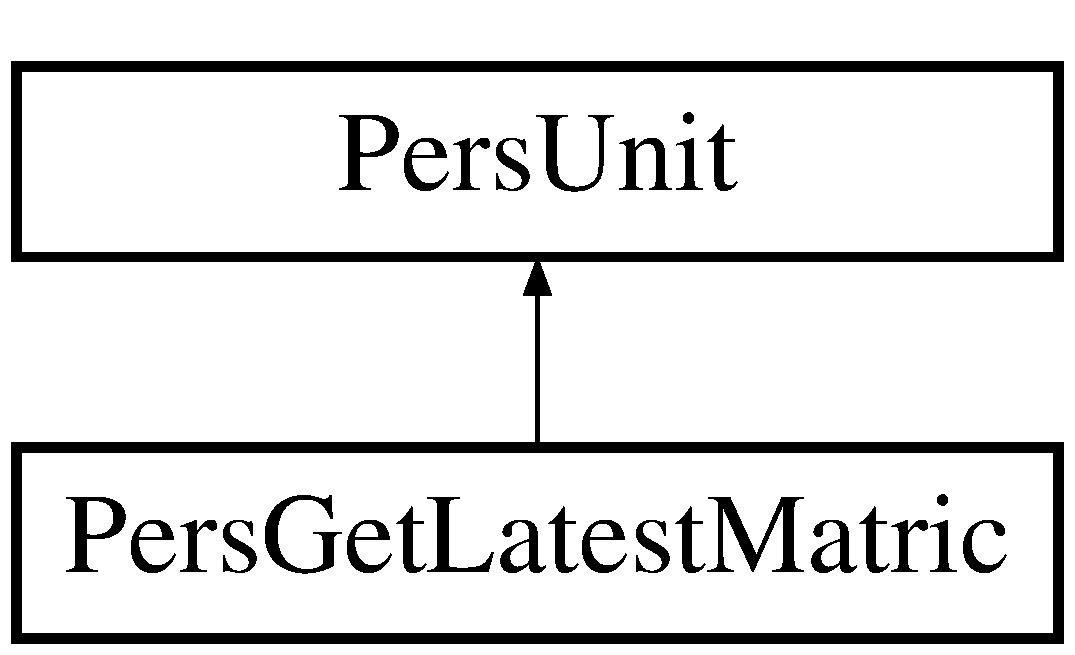
\includegraphics[height=2.000000cm]{de/d05/classPersGetLatestMatric}
\end{center}
\end{figure}
\subsubsection*{Public Member Functions}
\begin{DoxyCompactItemize}
\item 
\hypertarget{classPersGetLatestMatric_aef898ecbe507a95af50cd77dbb48620e}{void {\bfseries execute} ()  throw (\-Pers\-Error)}\label{de/d05/classPersGetLatestMatric_aef898ecbe507a95af50cd77dbb48620e}

\end{DoxyCompactItemize}
\subsubsection*{Additional Inherited Members}


\subsubsection{Detailed Description}


Definition at line 148 of file Pers\-Unit.\-h.



The documentation for this class was generated from the following files\-:\begin{DoxyCompactItemize}
\item 
Pers\-Unit.\-h\item 
Pers\-Unit.\-cpp\end{DoxyCompactItemize}

\hypertarget{classPersGetLatestNum}{\subsection{Pers\-Get\-Latest\-Num Class Reference}
\label{df/dec/classPersGetLatestNum}\index{Pers\-Get\-Latest\-Num@{Pers\-Get\-Latest\-Num}}
}
Inheritance diagram for Pers\-Get\-Latest\-Num\-:\begin{figure}[H]
\begin{center}
\leavevmode
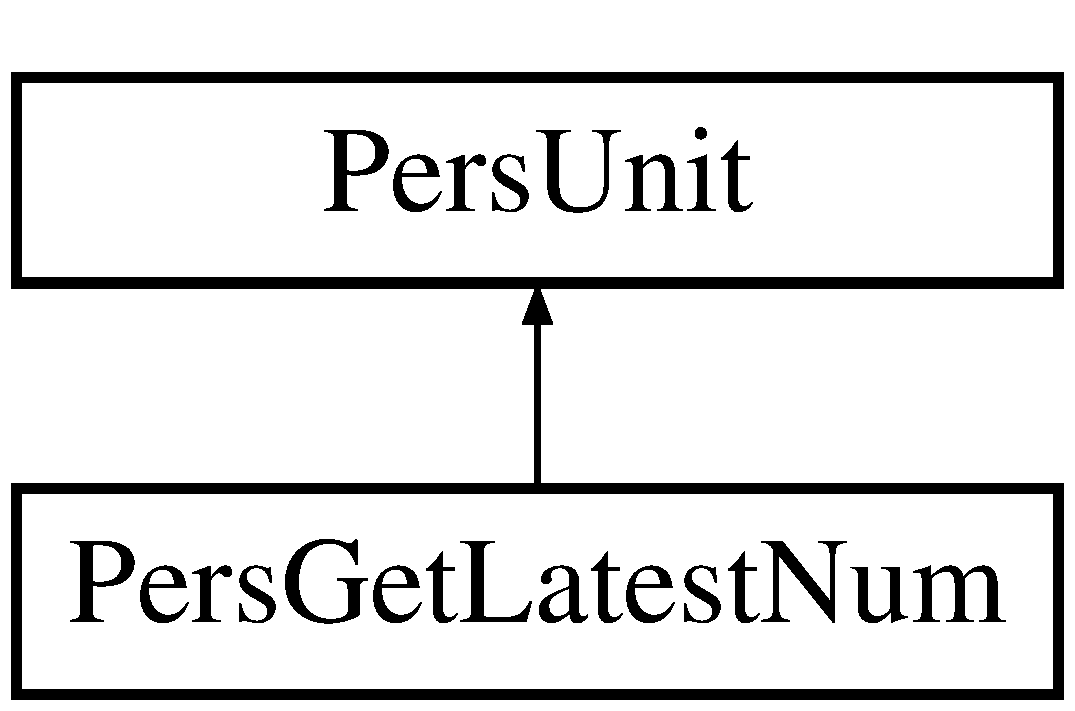
\includegraphics[height=2.000000cm]{df/dec/classPersGetLatestNum}
\end{center}
\end{figure}
\subsubsection*{Public Member Functions}
\begin{DoxyCompactItemize}
\item 
\hypertarget{classPersGetLatestNum_adf7f74e302ac82728b168e28d973ea3e}{void {\bfseries execute} ()  throw (\-Pers\-Error)}\label{df/dec/classPersGetLatestNum_adf7f74e302ac82728b168e28d973ea3e}

\item 
\hypertarget{classPersGetLatestNum_a93913c122245476bdc1cf0dfe1b94c6f}{\hyperlink{classAccNumber}{Acc\-Number} {\bfseries get\-Result} ()}\label{df/dec/classPersGetLatestNum_a93913c122245476bdc1cf0dfe1b94c6f}

\end{DoxyCompactItemize}
\subsubsection*{Additional Inherited Members}


\subsubsection{Detailed Description}


Definition at line 181 of file Pers\-Unit.\-h.



The documentation for this class was generated from the following files\-:\begin{DoxyCompactItemize}
\item 
Pers\-Unit.\-h\item 
Pers\-Unit.\-cpp\end{DoxyCompactItemize}

\hypertarget{classPersGetManager}{\subsection{Pers\-Get\-Manager Class Reference}
\label{db/db6/classPersGetManager}\index{Pers\-Get\-Manager@{Pers\-Get\-Manager}}
}


Classe Command que retorna o Gerente/\-Administrador correspondente cadastrado sob a matrícula fornecida.  




{\ttfamily \#include $<$Pers\-Unit.\-h$>$}

Inheritance diagram for Pers\-Get\-Manager\-:\begin{figure}[H]
\begin{center}
\leavevmode
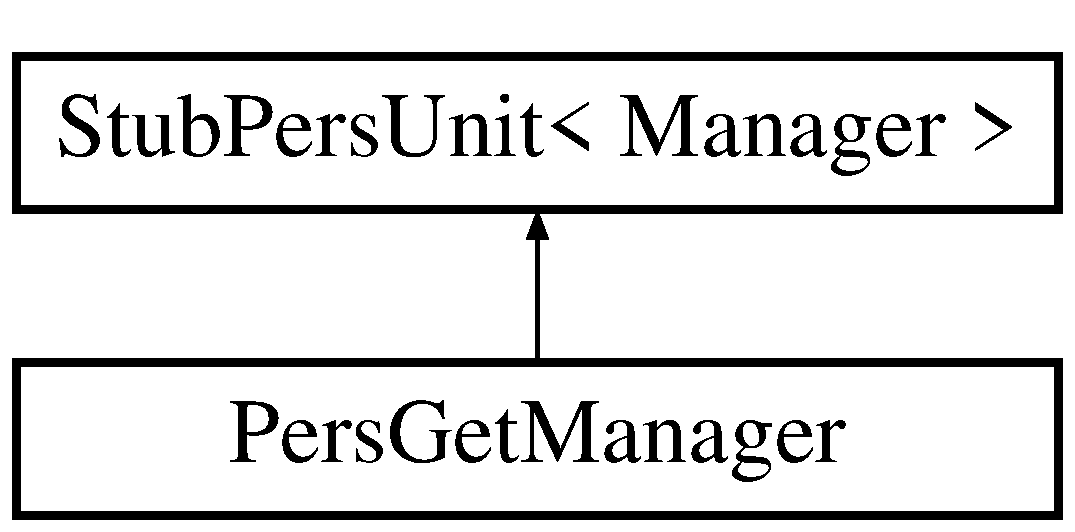
\includegraphics[height=2.000000cm]{db/db6/classPersGetManager}
\end{center}
\end{figure}
\subsubsection*{Public Member Functions}
\begin{DoxyCompactItemize}
\item 
\hypertarget{classPersGetManager_a7bad813d5561b69e2e3dd902d28601d9}{void {\bfseries execute} (\hyperlink{classUsrMatric}{Usr\-Matric} $\ast$)  throw (\-Pers\-Error, invalid\-\_\-argument)}\label{db/db6/classPersGetManager_a7bad813d5561b69e2e3dd902d28601d9}

\item 
\hypertarget{classPersGetManager_aa1a22e73d1763f77871d75fea89b1224}{\hyperlink{classManager}{Manager} {\bfseries get\-Result} ()}\label{db/db6/classPersGetManager_aa1a22e73d1763f77871d75fea89b1224}

\end{DoxyCompactItemize}
\subsubsection*{Additional Inherited Members}


\subsubsection{Detailed Description}
Classe Command que retorna o Gerente/\-Administrador correspondente cadastrado sob a matrícula fornecida. 

Definition at line 167 of file Pers\-Unit.\-h.



The documentation for this class was generated from the following files\-:\begin{DoxyCompactItemize}
\item 
Pers\-Unit.\-h\item 
Pers\-Unit.\-cpp\end{DoxyCompactItemize}

\hypertarget{classPersNewAccount}{\subsection{Pers\-New\-Account Class Reference}
\label{dc/d6d/classPersNewAccount}\index{Pers\-New\-Account@{Pers\-New\-Account}}
}
Inheritance diagram for Pers\-New\-Account\-:\begin{figure}[H]
\begin{center}
\leavevmode
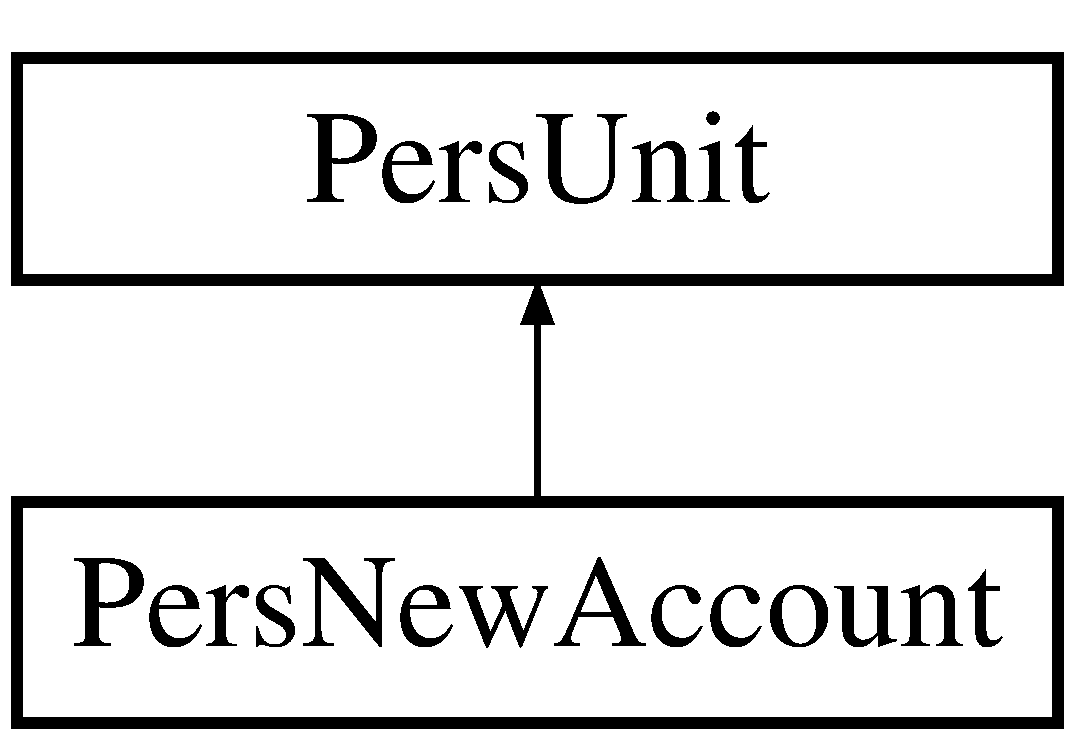
\includegraphics[height=2.000000cm]{dc/d6d/classPersNewAccount}
\end{center}
\end{figure}
\subsubsection*{Public Member Functions}
\begin{DoxyCompactItemize}
\item 
\hypertarget{classPersNewAccount_a87856dc414f6f409b86a9f6120f6e2f1}{void {\bfseries execute} (\hyperlink{classAccount}{Account} $\ast$)  throw (\-Pers\-Error)}\label{dc/d6d/classPersNewAccount_a87856dc414f6f409b86a9f6120f6e2f1}

\end{DoxyCompactItemize}
\subsubsection*{Additional Inherited Members}


\subsubsection{Detailed Description}


Definition at line 188 of file Pers\-Unit.\-h.



The documentation for this class was generated from the following files\-:\begin{DoxyCompactItemize}
\item 
Pers\-Unit.\-h\item 
Pers\-Unit.\-cpp\end{DoxyCompactItemize}

\hypertarget{classPersNewCustomer}{\subsection{Pers\-New\-Customer Class Reference}
\label{d2/df7/classPersNewCustomer}\index{Pers\-New\-Customer@{Pers\-New\-Customer}}
}
Inheritance diagram for Pers\-New\-Customer\-:\begin{figure}[H]
\begin{center}
\leavevmode
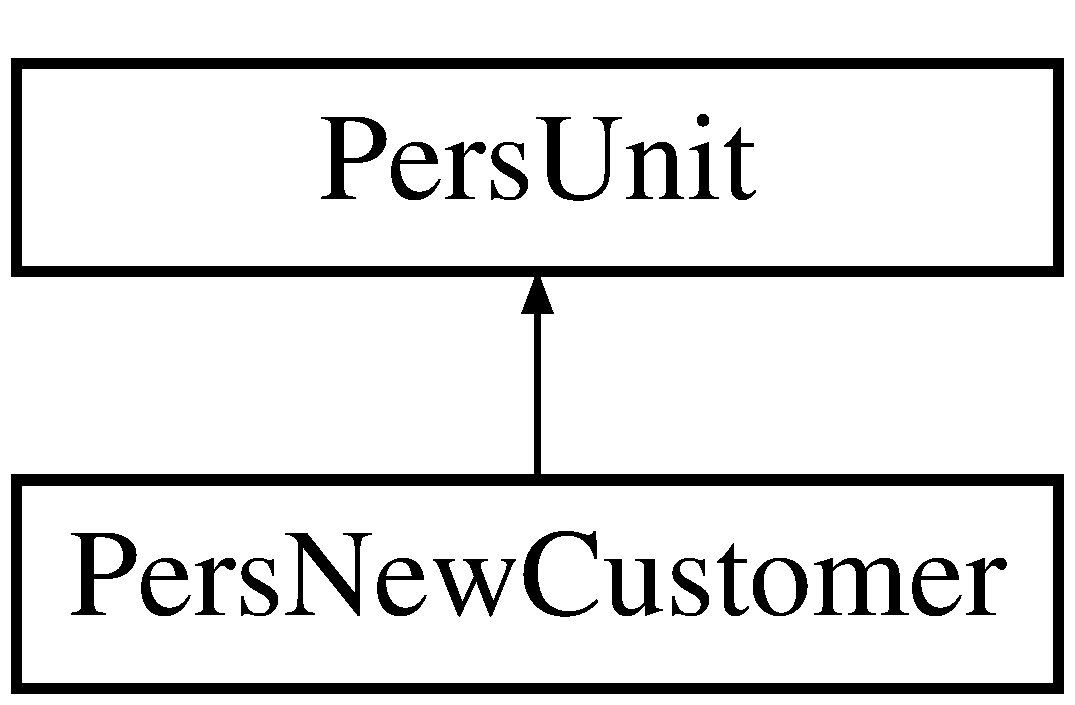
\includegraphics[height=2.000000cm]{d2/df7/classPersNewCustomer}
\end{center}
\end{figure}
\subsubsection*{Public Member Functions}
\begin{DoxyCompactItemize}
\item 
\hypertarget{classPersNewCustomer_ad51534c9c036e6eb8b9294242d5631ea}{void {\bfseries execute} (\hyperlink{classCustomer}{Customer} $\ast$)  throw (\-Pers\-Error)}\label{d2/df7/classPersNewCustomer_ad51534c9c036e6eb8b9294242d5631ea}

\end{DoxyCompactItemize}
\subsubsection*{Additional Inherited Members}


\subsubsection{Detailed Description}


Definition at line 186 of file Pers\-Unit.\-h.



The documentation for this class was generated from the following files\-:\begin{DoxyCompactItemize}
\item 
Pers\-Unit.\-h\item 
Pers\-Unit.\-cpp\end{DoxyCompactItemize}

\hypertarget{classPersNewManager}{\subsection{Pers\-New\-Manager Class Reference}
\label{d5/d99/classPersNewManager}\index{Pers\-New\-Manager@{Pers\-New\-Manager}}
}
Inheritance diagram for Pers\-New\-Manager\-:\begin{figure}[H]
\begin{center}
\leavevmode
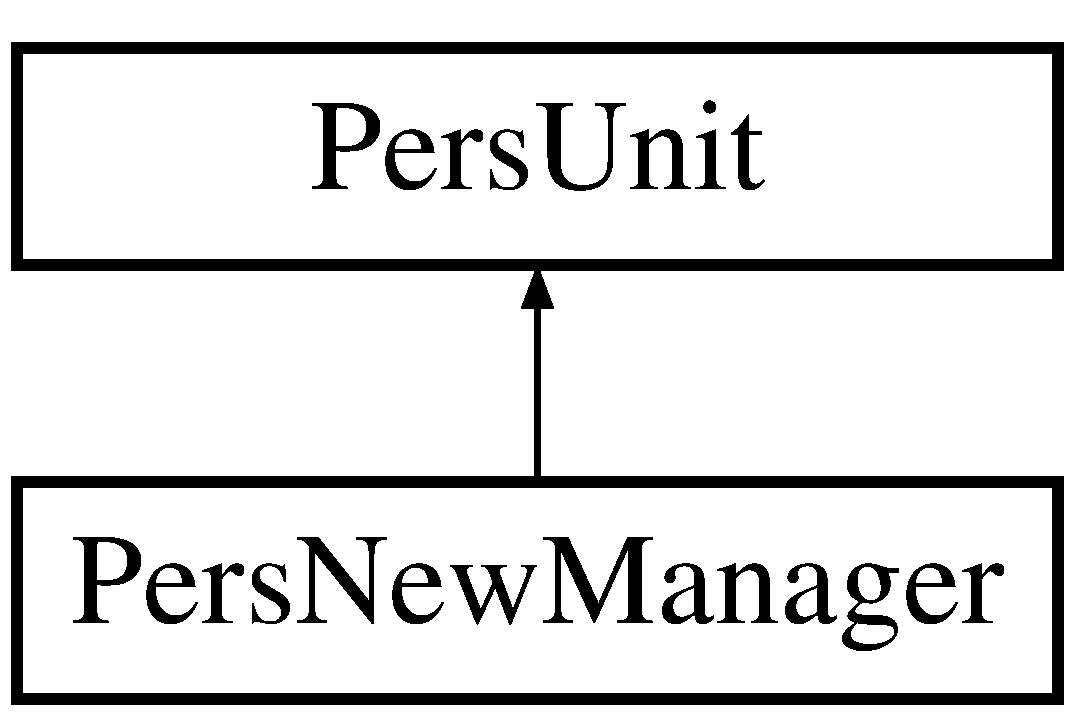
\includegraphics[height=2.000000cm]{d5/d99/classPersNewManager}
\end{center}
\end{figure}
\subsubsection*{Public Member Functions}
\begin{DoxyCompactItemize}
\item 
\hypertarget{classPersNewManager_a2465e298c83cd53a2e418a15fef87a75}{void {\bfseries execute} (\hyperlink{classManager}{Manager} $\ast$)  throw (\-Pers\-Error)}\label{d5/d99/classPersNewManager_a2465e298c83cd53a2e418a15fef87a75}

\end{DoxyCompactItemize}
\subsubsection*{Additional Inherited Members}


\subsubsection{Detailed Description}


Definition at line 233 of file Pers\-Unit.\-h.



The documentation for this class was generated from the following files\-:\begin{DoxyCompactItemize}
\item 
Pers\-Unit.\-h\item 
Pers\-Unit.\-cpp\end{DoxyCompactItemize}

\hypertarget{classPersNewPayment}{\subsection{Pers\-New\-Payment Class Reference}
\label{d5/d21/classPersNewPayment}\index{Pers\-New\-Payment@{Pers\-New\-Payment}}
}


Classe Command que cria um novo registro de \hyperlink{classPayment}{Payment}.  




{\ttfamily \#include $<$Pers\-Unit.\-h$>$}

Inheritance diagram for Pers\-New\-Payment\-:\begin{figure}[H]
\begin{center}
\leavevmode
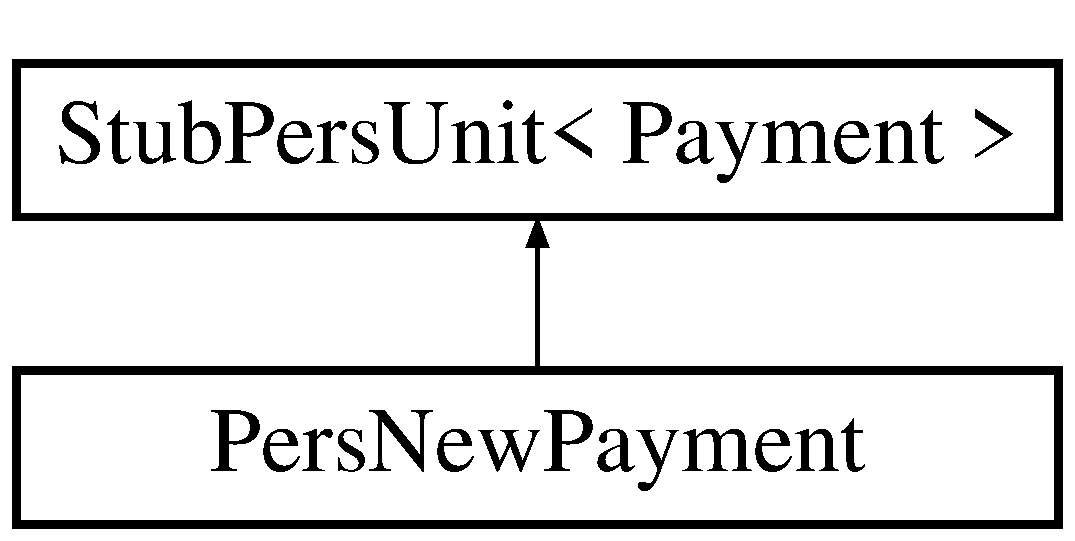
\includegraphics[height=2.000000cm]{d5/d21/classPersNewPayment}
\end{center}
\end{figure}
\subsubsection*{Public Member Functions}
\begin{DoxyCompactItemize}
\item 
\hypertarget{classPersNewPayment_adb33b781580bd87c025d15cdaeafb2f6}{void {\bfseries execute} (\hyperlink{classPayment}{Payment} $\ast$)  throw (\-Pers\-Error)}\label{d5/d21/classPersNewPayment_adb33b781580bd87c025d15cdaeafb2f6}

\end{DoxyCompactItemize}
\subsubsection*{Additional Inherited Members}


\subsubsection{Detailed Description}
Classe Command que cria um novo registro de \hyperlink{classPayment}{Payment}. 

Definition at line 145 of file Pers\-Unit.\-h.



The documentation for this class was generated from the following files\-:\begin{DoxyCompactItemize}
\item 
Pers\-Unit.\-h\item 
Pers\-Unit.\-cpp\end{DoxyCompactItemize}

\hypertarget{classPersSetBalance}{\subsection{Pers\-Set\-Balance Class Reference}
\label{d9/d6f/classPersSetBalance}\index{Pers\-Set\-Balance@{Pers\-Set\-Balance}}
}


Classe Command que define no database o Balance da conta de número \hyperlink{classAccNumber}{Acc\-Number}.  




{\ttfamily \#include $<$Pers\-Unit.\-h$>$}

Inheritance diagram for Pers\-Set\-Balance\-:\begin{figure}[H]
\begin{center}
\leavevmode
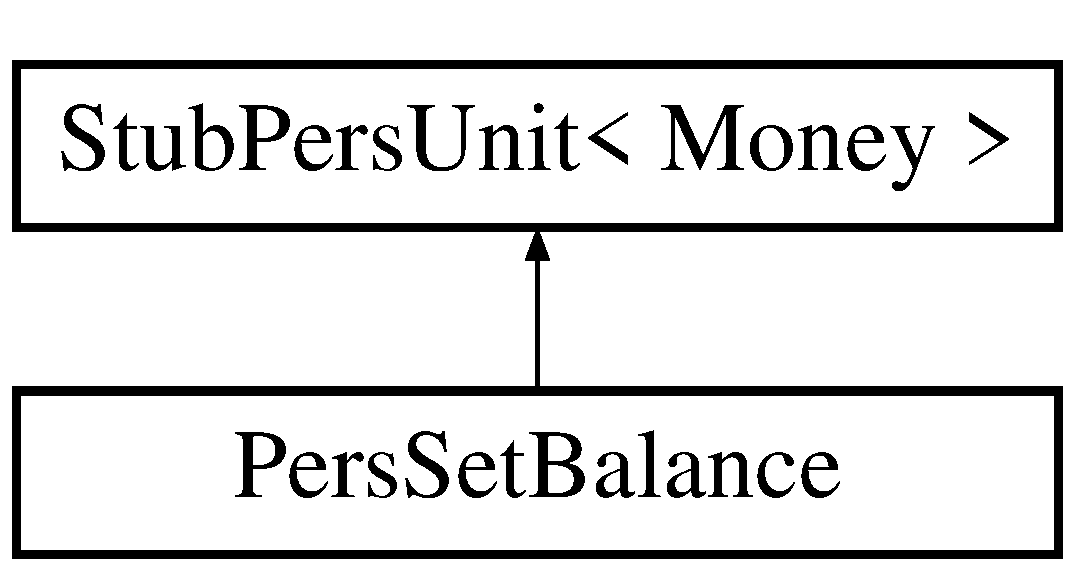
\includegraphics[height=2.000000cm]{d9/d6f/classPersSetBalance}
\end{center}
\end{figure}
\subsubsection*{Public Member Functions}
\begin{DoxyCompactItemize}
\item 
\hypertarget{classPersSetBalance_ac62b70b221a0e04e9e467f6d9e7162d1}{void {\bfseries execute} (\hyperlink{classAccNumber}{Acc\-Number}, \hyperlink{classMoney}{Money} $\ast$)  throw (\-Pers\-Error)}\label{d9/d6f/classPersSetBalance_ac62b70b221a0e04e9e467f6d9e7162d1}

\end{DoxyCompactItemize}
\subsubsection*{Additional Inherited Members}


\subsubsection{Detailed Description}
Classe Command que define no database o Balance da conta de número \hyperlink{classAccNumber}{Acc\-Number}. 

Definition at line 130 of file Pers\-Unit.\-h.



The documentation for this class was generated from the following files\-:\begin{DoxyCompactItemize}
\item 
Pers\-Unit.\-h\item 
Pers\-Unit.\-cpp\end{DoxyCompactItemize}

\hypertarget{classPersUblkAccount}{\subsection{Pers\-Ublk\-Account Class Reference}
\label{d6/d3f/classPersUblkAccount}\index{Pers\-Ublk\-Account@{Pers\-Ublk\-Account}}
}
Inheritance diagram for Pers\-Ublk\-Account\-:\begin{figure}[H]
\begin{center}
\leavevmode
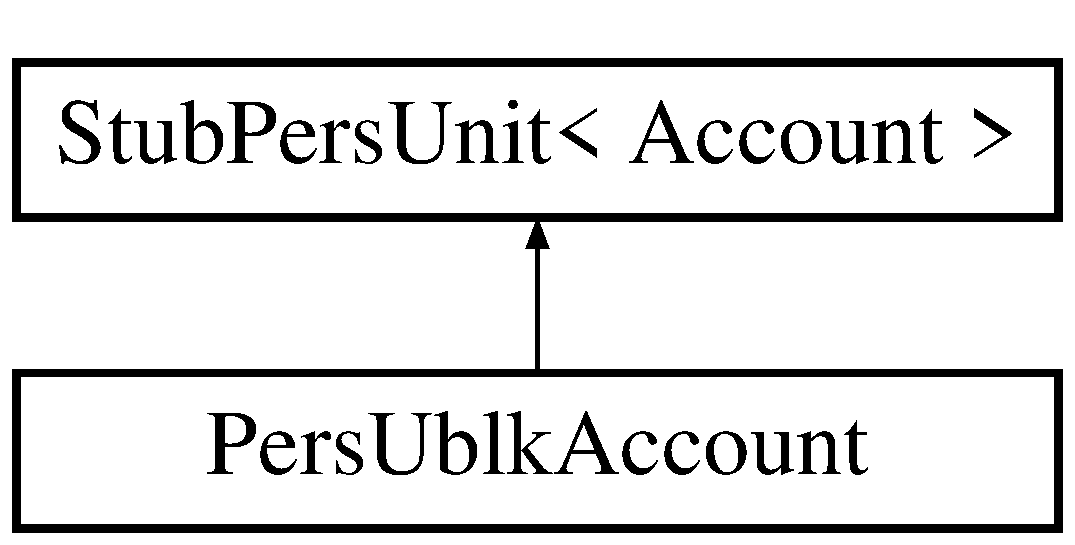
\includegraphics[height=2.000000cm]{d6/d3f/classPersUblkAccount}
\end{center}
\end{figure}
\subsubsection*{Public Member Functions}
\begin{DoxyCompactItemize}
\item 
\hypertarget{classPersUblkAccount_a54c2da815d702cdb200c88cd802f7dd2}{void {\bfseries execute} (\hyperlink{classAccNumber}{Acc\-Number} $\ast$)  throw (\-Pers\-Error)}\label{d6/d3f/classPersUblkAccount_a54c2da815d702cdb200c88cd802f7dd2}

\end{DoxyCompactItemize}
\subsubsection*{Additional Inherited Members}


\subsubsection{Detailed Description}


Definition at line 141 of file Pers\-Unit.\-h.



The documentation for this class was generated from the following files\-:\begin{DoxyCompactItemize}
\item 
Pers\-Unit.\-h\item 
Pers\-Unit.\-cpp\end{DoxyCompactItemize}

\hypertarget{classSession}{\section{Session Class Reference}
\label{de/d41/classSession}\index{Session@{Session}}
}


Classe que armazena, monitora e administra os dados de sessão.  




{\ttfamily \#include $<$Main\-Unit.\-h$>$}

\subsection*{Public Member Functions}
\begin{DoxyCompactItemize}
\item 
\hyperlink{classSession_a216a4f17b0c16bd7e2e5ace3c5500efa}{Session} (\hyperlink{classUsrMatric}{Usr\-Matric} $\ast$, \hyperlink{classUsrPassword}{Usr\-Password} $\ast$)
\begin{DoxyCompactList}\small\item\em Construtor para gerentes ou administradores. \end{DoxyCompactList}\item 
\hyperlink{classSession_ad94e7557f00ffe2abd64acf12d6f79d4}{Session} (\hyperlink{classAccNumber}{Acc\-Number} $\ast$, \hyperlink{classUsrPassword}{Usr\-Password} $\ast$)
\begin{DoxyCompactList}\small\item\em Construtor para clientes. \end{DoxyCompactList}\item 
\hypertarget{classSession_a8aff9f54e6d36a716794e7477820dc72}{void {\bfseries set\-Usr\-Matric} (\hyperlink{classUsrMatric}{Usr\-Matric} $\ast$)}\label{de/d41/classSession_a8aff9f54e6d36a716794e7477820dc72}

\item 
\hypertarget{classSession_a350981c1ca9d9eb3e3b78495a84a3acd}{void {\bfseries set\-Acc\-Number} (\hyperlink{classAccNumber}{Acc\-Number} $\ast$)}\label{de/d41/classSession_a350981c1ca9d9eb3e3b78495a84a3acd}

\item 
\hypertarget{classSession_a0c2ea92fd94940c314e6d5728bbe3725}{void {\bfseries set\-Usr\-Password} (\hyperlink{classUsrPassword}{Usr\-Password} $\ast$)}\label{de/d41/classSession_a0c2ea92fd94940c314e6d5728bbe3725}

\item 
\hypertarget{classSession_ab652b031c32df3f5c3c6ff4011477be9}{\hyperlink{classUsrMatric}{Usr\-Matric} {\bfseries get\-Usr\-Matric} () const }\label{de/d41/classSession_ab652b031c32df3f5c3c6ff4011477be9}

\item 
\hypertarget{classSession_a3b3e2fbabef41e2040cc1bfc7a206bc3}{\hyperlink{classAccNumber}{Acc\-Number} {\bfseries get\-Acc\-Number} () const }\label{de/d41/classSession_a3b3e2fbabef41e2040cc1bfc7a206bc3}

\item 
\hypertarget{classSession_a6907e9cd690bbe1d6d36c276687d5816}{\hyperlink{classUsrPassword}{Usr\-Password} {\bfseries get\-Usr\-Password} () const }\label{de/d41/classSession_a6907e9cd690bbe1d6d36c276687d5816}

\end{DoxyCompactItemize}


\subsection{Detailed Description}
Classe que armazena, monitora e administra os dados de sessão. 



\subsection{Constructor \& Destructor Documentation}
\hypertarget{classSession_a216a4f17b0c16bd7e2e5ace3c5500efa}{\index{Session@{Session}!Session@{Session}}
\index{Session@{Session}!Session@{Session}}
\subsubsection[{Session}]{\setlength{\rightskip}{0pt plus 5cm}Session\-::\-Session (
\begin{DoxyParamCaption}
\item[{{\bf Usr\-Matric} $\ast$}]{usr\-Matric, }
\item[{{\bf Usr\-Password} $\ast$}]{usr\-Password}
\end{DoxyParamCaption}
)}}\label{de/d41/classSession_a216a4f17b0c16bd7e2e5ace3c5500efa}


Construtor para gerentes ou administradores. 

\hypertarget{classSession_ad94e7557f00ffe2abd64acf12d6f79d4}{\index{Session@{Session}!Session@{Session}}
\index{Session@{Session}!Session@{Session}}
\subsubsection[{Session}]{\setlength{\rightskip}{0pt plus 5cm}Session\-::\-Session (
\begin{DoxyParamCaption}
\item[{{\bf Acc\-Number} $\ast$}]{acc\-Number, }
\item[{{\bf Usr\-Password} $\ast$}]{usr\-Password}
\end{DoxyParamCaption}
)}}\label{de/d41/classSession_ad94e7557f00ffe2abd64acf12d6f79d4}


Construtor para clientes. 



The documentation for this class was generated from the following files\-:\begin{DoxyCompactItemize}
\item 
Main\-Unit.\-h\item 
Main\-Unit.\-cpp\end{DoxyCompactItemize}

\hypertarget{classStubPersUnit}{\subsection{Stub\-Pers\-Unit$<$ Return\-Class $>$ Class Template Reference}
\label{d5/dfd/classStubPersUnit}\index{Stub\-Pers\-Unit$<$ Return\-Class $>$@{Stub\-Pers\-Unit$<$ Return\-Class $>$}}
}


Stub da camada de persistência.  




{\ttfamily \#include $<$Pers\-Unit.\-h$>$}

\subsubsection*{Public Member Functions}
\begin{DoxyCompactItemize}
\item 
\hypertarget{classStubPersUnit_a85372c81d59b3c7c765d013c8d34fec5}{void {\bfseries set\-D\-B\-Name} (string name)}\label{d5/dfd/classStubPersUnit_a85372c81d59b3c7c765d013c8d34fec5}

\item 
\hypertarget{classStubPersUnit_a6911707b204e735e1eab885e544dbd6c}{list$<$ Return\-Class $>$ {\bfseries get\-Result} ()}\label{d5/dfd/classStubPersUnit_a6911707b204e735e1eab885e544dbd6c}

\end{DoxyCompactItemize}
\subsubsection*{Protected Attributes}
\begin{DoxyCompactItemize}
\item 
\hypertarget{classStubPersUnit_af932467573f602fe0853e30be7d56f10}{list$<$ Return\-Class $>$ {\bfseries return\-List}}\label{d5/dfd/classStubPersUnit_af932467573f602fe0853e30be7d56f10}

\end{DoxyCompactItemize}


\subsubsection{Detailed Description}
\subsubsection*{template$<$class Return\-Class$>$class Stub\-Pers\-Unit$<$ Return\-Class $>$}

Stub da camada de persistência. 

Definition at line 31 of file Pers\-Unit.\-h.



The documentation for this class was generated from the following file\-:\begin{DoxyCompactItemize}
\item 
Pers\-Unit.\-h\end{DoxyCompactItemize}

\hypertarget{classStubTransacAdm}{\subsection{Stub\-Transac\-Adm Class Reference}
\label{d9/d0f/classStubTransacAdm}\index{Stub\-Transac\-Adm@{Stub\-Transac\-Adm}}
}


Stub utilizado para simular o funcionamento da camada de negócio.  




{\ttfamily \#include $<$Transac\-Unit.\-h$>$}

Inheritance diagram for Stub\-Transac\-Adm\-:\begin{figure}[H]
\begin{center}
\leavevmode
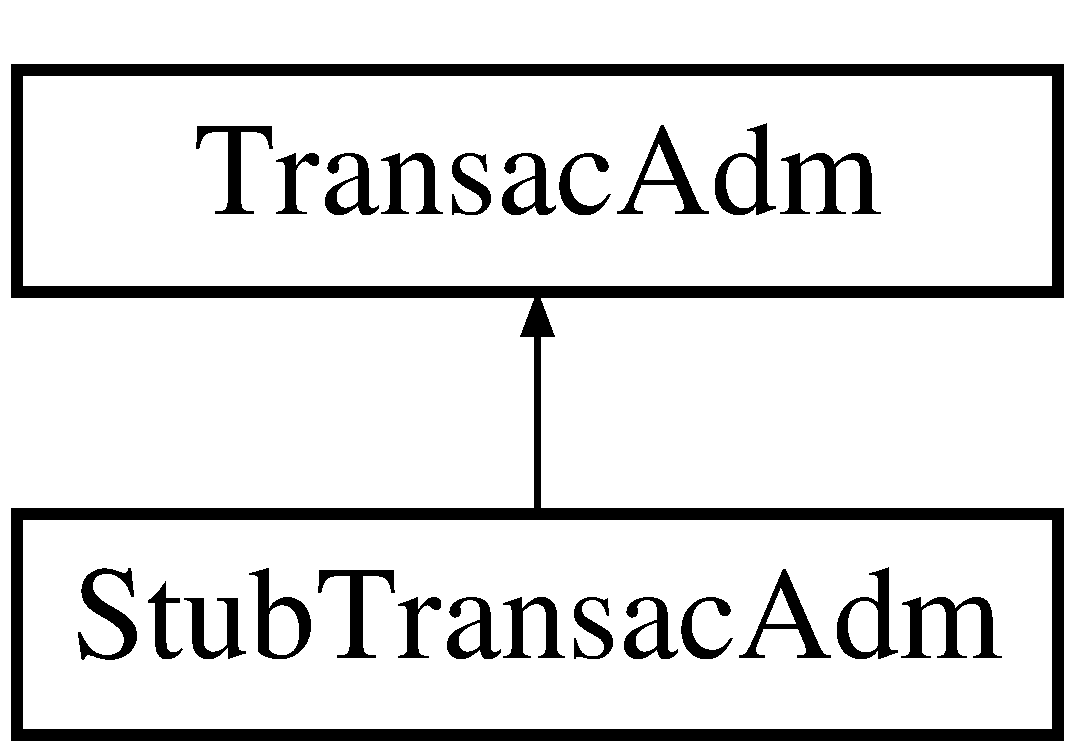
\includegraphics[height=2.000000cm]{d9/d0f/classStubTransacAdm}
\end{center}
\end{figure}
\subsubsection*{Public Member Functions}
\begin{DoxyCompactItemize}
\item 
void \hyperlink{classStubTransacAdm_aa411e937e159c26aa50901aad504db42}{withdraw} (\hyperlink{classAccNumber}{Acc\-Number}, \hyperlink{classMoney}{Money} $\ast$)  throw (invalid\-\_\-argument, Pers\-Error)
\begin{DoxyCompactList}\small\item\em Executa a retirada de dinheiro. \end{DoxyCompactList}\item 
void \hyperlink{classStubTransacAdm_afc25824382e5ce8cd491a573b557bbc1}{deposit} (\hyperlink{classAccNumber}{Acc\-Number}, \hyperlink{classMoney}{Money} $\ast$)  throw (invalid\-\_\-argument, Pers\-Error)
\begin{DoxyCompactList}\small\item\em Executa um depósito. \end{DoxyCompactList}\item 
\hyperlink{classPayCode}{Pay\-Code} $\ast$ \hyperlink{classStubTransacAdm_ad794a9d6f46b1f4d62aef292f8fed5f4}{schedule\-Payment} (\hyperlink{classAccNumber}{Acc\-Number}, \hyperlink{classMoney}{Money} $\ast$, \hyperlink{classPayDay}{Pay\-Day} $\ast$)  throw (invalid\-\_\-argument, Pers\-Error)
\begin{DoxyCompactList}\small\item\em Agenda um pagamento. \end{DoxyCompactList}\item 
void \hyperlink{classStubTransacAdm_a734de9620871592c6d40b2c819c69650}{delete\-Payment} (\hyperlink{classPayCode}{Pay\-Code} $\ast$)  throw (invalid\-\_\-argument, Pers\-Error)
\begin{DoxyCompactList}\small\item\em Deleta um pagamento agendado. \end{DoxyCompactList}\item 
list$<$ \hyperlink{classPayment}{Payment} $>$ \hyperlink{classStubTransacAdm_a0896f821752fc696322bd58444a1d5ab}{fetch\-Payment} (void)  throw (\-Pers\-Error)
\begin{DoxyCompactList}\small\item\em Recupera uma lista de todos os pagamentos registrados. \end{DoxyCompactList}\end{DoxyCompactItemize}


\subsubsection{Detailed Description}
Stub utilizado para simular o funcionamento da camada de negócio. 

Definition at line 47 of file Transac\-Unit.\-h.



\subsubsection{Member Function Documentation}
\hypertarget{classStubTransacAdm_a734de9620871592c6d40b2c819c69650}{\index{Stub\-Transac\-Adm@{Stub\-Transac\-Adm}!delete\-Payment@{delete\-Payment}}
\index{delete\-Payment@{delete\-Payment}!StubTransacAdm@{Stub\-Transac\-Adm}}
\paragraph[{delete\-Payment}]{\setlength{\rightskip}{0pt plus 5cm}void Stub\-Transac\-Adm\-::delete\-Payment (
\begin{DoxyParamCaption}
\item[{{\bf Pay\-Code} $\ast$}]{}
\end{DoxyParamCaption}
)  throw (invalid\-\_\-argument, {\bf Pers\-Error})\hspace{0.3cm}{\ttfamily [virtual]}}}\label{d9/d0f/classStubTransacAdm_a734de9620871592c6d40b2c819c69650}


Deleta um pagamento agendado. 



Implements \hyperlink{classTransacAdm_a76f27b0fc9e604695c4c601839d3b441}{Transac\-Adm}.



Definition at line 90 of file Transac\-Unit.\-cpp.

\hypertarget{classStubTransacAdm_afc25824382e5ce8cd491a573b557bbc1}{\index{Stub\-Transac\-Adm@{Stub\-Transac\-Adm}!deposit@{deposit}}
\index{deposit@{deposit}!StubTransacAdm@{Stub\-Transac\-Adm}}
\paragraph[{deposit}]{\setlength{\rightskip}{0pt plus 5cm}void Stub\-Transac\-Adm\-::deposit (
\begin{DoxyParamCaption}
\item[{{\bf Acc\-Number}}]{, }
\item[{{\bf Money} $\ast$}]{}
\end{DoxyParamCaption}
)  throw (invalid\-\_\-argument, {\bf Pers\-Error})\hspace{0.3cm}{\ttfamily [virtual]}}}\label{d9/d0f/classStubTransacAdm_afc25824382e5ce8cd491a573b557bbc1}


Executa um depósito. 



Implements \hyperlink{classTransacAdm_a9b6ffc8a521600094eb13510edcb33d7}{Transac\-Adm}.



Definition at line 46 of file Transac\-Unit.\-cpp.

\hypertarget{classStubTransacAdm_a0896f821752fc696322bd58444a1d5ab}{\index{Stub\-Transac\-Adm@{Stub\-Transac\-Adm}!fetch\-Payment@{fetch\-Payment}}
\index{fetch\-Payment@{fetch\-Payment}!StubTransacAdm@{Stub\-Transac\-Adm}}
\paragraph[{fetch\-Payment}]{\setlength{\rightskip}{0pt plus 5cm}list$<$ {\bf Payment} $>$ Stub\-Transac\-Adm\-::fetch\-Payment (
\begin{DoxyParamCaption}
\item[{void}]{}
\end{DoxyParamCaption}
)  throw ({\bf Pers\-Error})\hspace{0.3cm}{\ttfamily [virtual]}}}\label{d9/d0f/classStubTransacAdm_a0896f821752fc696322bd58444a1d5ab}


Recupera uma lista de todos os pagamentos registrados. 



Implements \hyperlink{classTransacAdm_ab3c02884c14540c1f520339581e88371}{Transac\-Adm}.



Definition at line 107 of file Transac\-Unit.\-cpp.

\hypertarget{classStubTransacAdm_ad794a9d6f46b1f4d62aef292f8fed5f4}{\index{Stub\-Transac\-Adm@{Stub\-Transac\-Adm}!schedule\-Payment@{schedule\-Payment}}
\index{schedule\-Payment@{schedule\-Payment}!StubTransacAdm@{Stub\-Transac\-Adm}}
\paragraph[{schedule\-Payment}]{\setlength{\rightskip}{0pt plus 5cm}{\bf Pay\-Code} $\ast$ Stub\-Transac\-Adm\-::schedule\-Payment (
\begin{DoxyParamCaption}
\item[{{\bf Acc\-Number}}]{, }
\item[{{\bf Money} $\ast$}]{, }
\item[{{\bf Pay\-Day} $\ast$}]{}
\end{DoxyParamCaption}
)  throw (invalid\-\_\-argument, {\bf Pers\-Error})\hspace{0.3cm}{\ttfamily [virtual]}}}\label{d9/d0f/classStubTransacAdm_ad794a9d6f46b1f4d62aef292f8fed5f4}


Agenda um pagamento. 



Implements \hyperlink{classTransacAdm_a6f350bc661f1a6460a31a0b02ccb8d3f}{Transac\-Adm}.



Definition at line 73 of file Transac\-Unit.\-cpp.

\hypertarget{classStubTransacAdm_aa411e937e159c26aa50901aad504db42}{\index{Stub\-Transac\-Adm@{Stub\-Transac\-Adm}!withdraw@{withdraw}}
\index{withdraw@{withdraw}!StubTransacAdm@{Stub\-Transac\-Adm}}
\paragraph[{withdraw}]{\setlength{\rightskip}{0pt plus 5cm}void Stub\-Transac\-Adm\-::withdraw (
\begin{DoxyParamCaption}
\item[{{\bf Acc\-Number}}]{, }
\item[{{\bf Money} $\ast$}]{}
\end{DoxyParamCaption}
)  throw (invalid\-\_\-argument, {\bf Pers\-Error})\hspace{0.3cm}{\ttfamily [virtual]}}}\label{d9/d0f/classStubTransacAdm_aa411e937e159c26aa50901aad504db42}


Executa a retirada de dinheiro. 



Implements \hyperlink{classTransacAdm_a128750caeeec2cd48a4a01e6ce9f701c}{Transac\-Adm}.



Definition at line 23 of file Transac\-Unit.\-cpp.



The documentation for this class was generated from the following files\-:\begin{DoxyCompactItemize}
\item 
Transac\-Unit.\-h\item 
Transac\-Unit.\-cpp\end{DoxyCompactItemize}

\hypertarget{classStubUserAccAdm}{\subsection{Stub\-User\-Acc\-Adm Class Reference}
\label{d3/d88/classStubUserAccAdm}\index{Stub\-User\-Acc\-Adm@{Stub\-User\-Acc\-Adm}}
}


Stub utilizado para simular o funcionamento da camada de negócio responsável pela administração dos dados de contas.  




{\ttfamily \#include $<$User\-Unit.\-h$>$}

Inheritance diagram for Stub\-User\-Acc\-Adm\-:\begin{figure}[H]
\begin{center}
\leavevmode
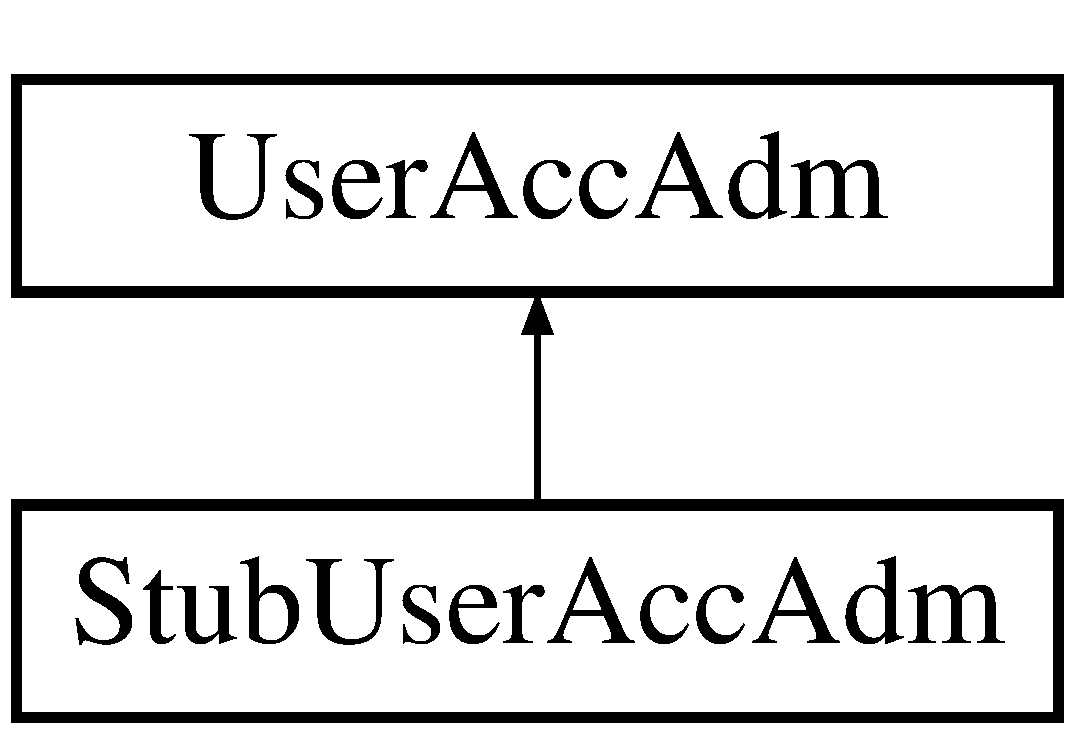
\includegraphics[height=2.000000cm]{d3/d88/classStubUserAccAdm}
\end{center}
\end{figure}


\subsubsection{Detailed Description}
Stub utilizado para simular o funcionamento da camada de negócio responsável pela administração dos dados de contas. 

Definition at line 54 of file User\-Unit.\-h.



The documentation for this class was generated from the following files\-:\begin{DoxyCompactItemize}
\item 
User\-Unit.\-h\item 
User\-Unit.\-cpp\end{DoxyCompactItemize}

\hypertarget{classStubUserCusAdm}{\subsection{Stub\-User\-Cus\-Adm Class Reference}
\label{d1/d9d/classStubUserCusAdm}\index{Stub\-User\-Cus\-Adm@{Stub\-User\-Cus\-Adm}}
}


Stub utilizado para simular o funcionamento da camada de negócio responsável pela administração de dados de clientes.  




{\ttfamily \#include $<$User\-Unit.\-h$>$}

Inheritance diagram for Stub\-User\-Cus\-Adm\-:\begin{figure}[H]
\begin{center}
\leavevmode
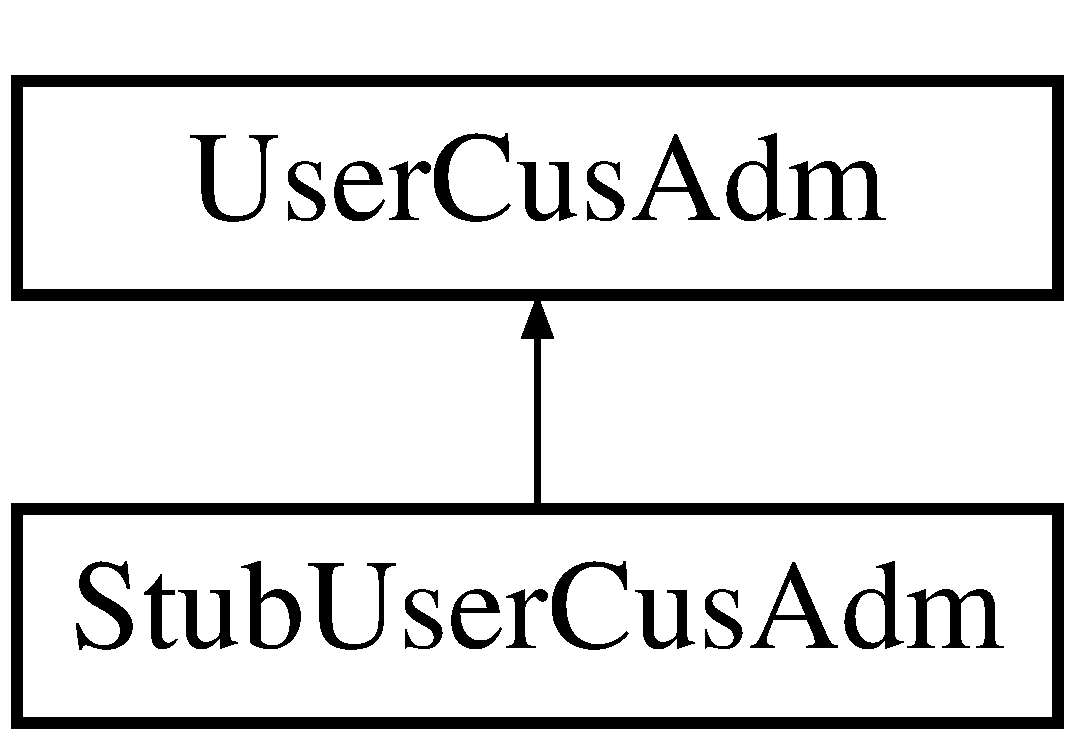
\includegraphics[height=2.000000cm]{d1/d9d/classStubUserCusAdm}
\end{center}
\end{figure}
\subsubsection*{Public Member Functions}
\begin{DoxyCompactItemize}
\item 
void \hyperlink{classStubUserCusAdm_a2786aaadaffac84a859f992159ebecf8}{change\-Password} (\hyperlink{classUsrId}{Usr\-Id}, \hyperlink{classUsrPassword}{Usr\-Password} $\ast$)  throw (\-Pers\-Error)
\begin{DoxyCompactList}\small\item\em Modifica a senha do cliente. \end{DoxyCompactList}\item 
\hyperlink{classUsrId}{Usr\-Id} \hyperlink{classStubUserCusAdm_a6b0c9fc7280045d06bf263d7286b37e9}{create\-Customer} (\hyperlink{classUsrName}{Usr\-Name} $\ast$, \hyperlink{classUsrPassword}{Usr\-Password} $\ast$)  throw (invalid\-\_\-argument, Pers\-Error)
\begin{DoxyCompactList}\small\item\em Cria um cliente. \end{DoxyCompactList}\item 
void \hyperlink{classStubUserCusAdm_a09db6dc02a43ff702efdc2341038df8e}{edit\-Cus\-Name} (\hyperlink{classUsrId}{Usr\-Id} $\ast$, \hyperlink{classUsrName}{Usr\-Name} $\ast$)  throw (invalid\-\_\-argument, Pers\-Error)
\begin{DoxyCompactList}\small\item\em Edita o nome do cliente. \end{DoxyCompactList}\item 
\hyperlink{classCustomer}{Customer} \hyperlink{classStubUserCusAdm_aac14b018a6284211b1c83c48a9529efe}{fetch\-Customer} (\hyperlink{classUsrId}{Usr\-Id})  throw (\-Pers\-Error)
\begin{DoxyCompactList}\small\item\em Recupera so dados do cliente. \end{DoxyCompactList}\end{DoxyCompactItemize}


\subsubsection{Detailed Description}
Stub utilizado para simular o funcionamento da camada de negócio responsável pela administração de dados de clientes. 

Definition at line 169 of file User\-Unit.\-h.



\subsubsection{Member Function Documentation}
\hypertarget{classStubUserCusAdm_a2786aaadaffac84a859f992159ebecf8}{\index{Stub\-User\-Cus\-Adm@{Stub\-User\-Cus\-Adm}!change\-Password@{change\-Password}}
\index{change\-Password@{change\-Password}!StubUserCusAdm@{Stub\-User\-Cus\-Adm}}
\paragraph[{change\-Password}]{\setlength{\rightskip}{0pt plus 5cm}void Stub\-User\-Cus\-Adm\-::change\-Password (
\begin{DoxyParamCaption}
\item[{{\bf Usr\-Id}}]{, }
\item[{{\bf Usr\-Password} $\ast$}]{}
\end{DoxyParamCaption}
)  throw ({\bf Pers\-Error})\hspace{0.3cm}{\ttfamily [virtual]}}}\label{d1/d9d/classStubUserCusAdm_a2786aaadaffac84a859f992159ebecf8}


Modifica a senha do cliente. 



Implements \hyperlink{classUserCusAdm_aed6d785e91a48c205df8c64736dbf3cf}{User\-Cus\-Adm}.



Definition at line 458 of file User\-Unit.\-cpp.

\hypertarget{classStubUserCusAdm_a6b0c9fc7280045d06bf263d7286b37e9}{\index{Stub\-User\-Cus\-Adm@{Stub\-User\-Cus\-Adm}!create\-Customer@{create\-Customer}}
\index{create\-Customer@{create\-Customer}!StubUserCusAdm@{Stub\-User\-Cus\-Adm}}
\paragraph[{create\-Customer}]{\setlength{\rightskip}{0pt plus 5cm}{\bf Usr\-Id} Stub\-User\-Cus\-Adm\-::create\-Customer (
\begin{DoxyParamCaption}
\item[{{\bf Usr\-Name} $\ast$}]{, }
\item[{{\bf Usr\-Password} $\ast$}]{}
\end{DoxyParamCaption}
)  throw (invalid\-\_\-argument, {\bf Pers\-Error})\hspace{0.3cm}{\ttfamily [virtual]}}}\label{d1/d9d/classStubUserCusAdm_a6b0c9fc7280045d06bf263d7286b37e9}


Cria um cliente. 



Implements \hyperlink{classUserCusAdm_a4775bb30caf44192349db204b95b2b2f}{User\-Cus\-Adm}.



Definition at line 464 of file User\-Unit.\-cpp.

\hypertarget{classStubUserCusAdm_a09db6dc02a43ff702efdc2341038df8e}{\index{Stub\-User\-Cus\-Adm@{Stub\-User\-Cus\-Adm}!edit\-Cus\-Name@{edit\-Cus\-Name}}
\index{edit\-Cus\-Name@{edit\-Cus\-Name}!StubUserCusAdm@{Stub\-User\-Cus\-Adm}}
\paragraph[{edit\-Cus\-Name}]{\setlength{\rightskip}{0pt plus 5cm}void Stub\-User\-Cus\-Adm\-::edit\-Cus\-Name (
\begin{DoxyParamCaption}
\item[{{\bf Usr\-Id} $\ast$}]{, }
\item[{{\bf Usr\-Name} $\ast$}]{}
\end{DoxyParamCaption}
)  throw (invalid\-\_\-argument, {\bf Pers\-Error})\hspace{0.3cm}{\ttfamily [virtual]}}}\label{d1/d9d/classStubUserCusAdm_a09db6dc02a43ff702efdc2341038df8e}


Edita o nome do cliente. 



Implements \hyperlink{classUserCusAdm_a2fffe3697904fb67ca285261276e1252}{User\-Cus\-Adm}.



Definition at line 476 of file User\-Unit.\-cpp.

\hypertarget{classStubUserCusAdm_aac14b018a6284211b1c83c48a9529efe}{\index{Stub\-User\-Cus\-Adm@{Stub\-User\-Cus\-Adm}!fetch\-Customer@{fetch\-Customer}}
\index{fetch\-Customer@{fetch\-Customer}!StubUserCusAdm@{Stub\-User\-Cus\-Adm}}
\paragraph[{fetch\-Customer}]{\setlength{\rightskip}{0pt plus 5cm}{\bf Customer} Stub\-User\-Cus\-Adm\-::fetch\-Customer (
\begin{DoxyParamCaption}
\item[{{\bf Usr\-Id}}]{}
\end{DoxyParamCaption}
)  throw ({\bf Pers\-Error})\hspace{0.3cm}{\ttfamily [virtual]}}}\label{d1/d9d/classStubUserCusAdm_aac14b018a6284211b1c83c48a9529efe}


Recupera so dados do cliente. 



Implements \hyperlink{classUserCusAdm_a8a67bf25c965e931be912f33449e0f8a}{User\-Cus\-Adm}.



Definition at line 484 of file User\-Unit.\-cpp.



The documentation for this class was generated from the following files\-:\begin{DoxyCompactItemize}
\item 
User\-Unit.\-h\item 
User\-Unit.\-cpp\end{DoxyCompactItemize}

\hypertarget{classStubUserLogin}{\subsection{Stub\-User\-Login Class Reference}
\label{d1/dbd/classStubUserLogin}\index{Stub\-User\-Login@{Stub\-User\-Login}}
}


Stub utilizado para simular o funcionamento da camada de negócio de login.  




{\ttfamily \#include $<$User\-Unit.\-h$>$}

Inheritance diagram for Stub\-User\-Login\-:\begin{figure}[H]
\begin{center}
\leavevmode
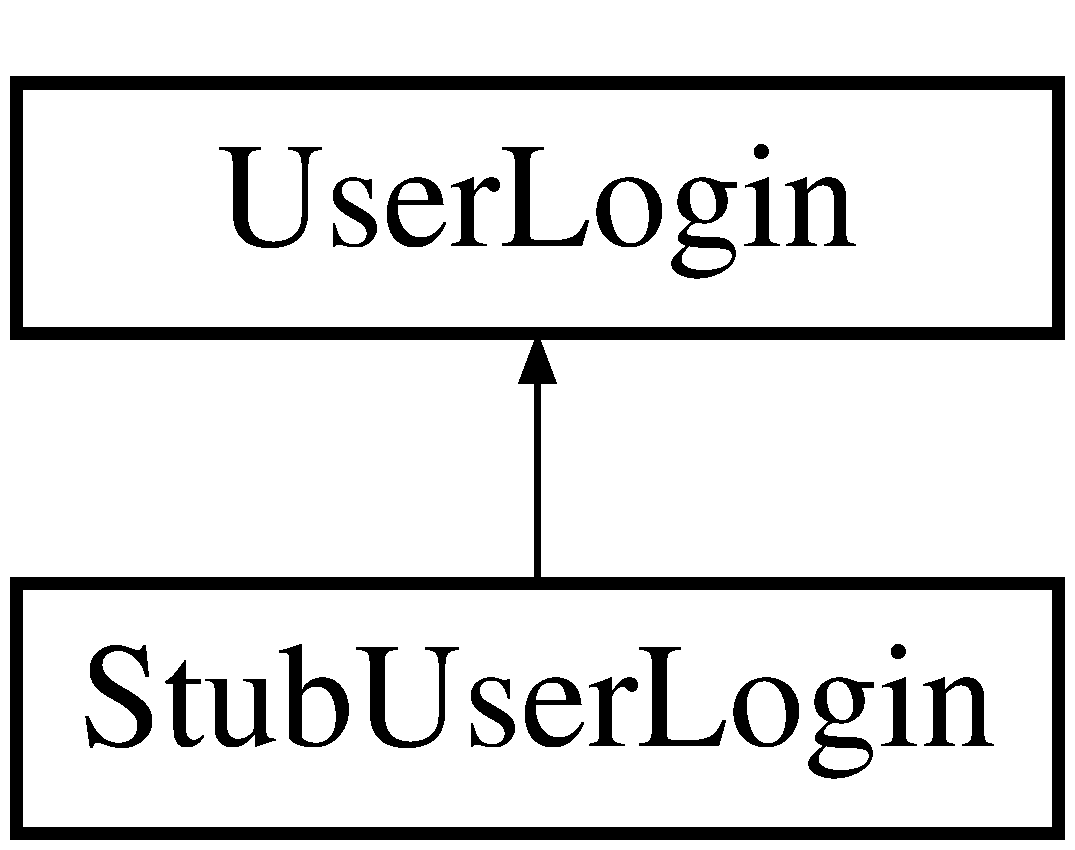
\includegraphics[height=2.000000cm]{d1/dbd/classStubUserLogin}
\end{center}
\end{figure}
\subsubsection*{Public Member Functions}
\begin{DoxyCompactItemize}
\item 
\hyperlink{classUsrType}{Man\-Type} \hyperlink{classStubUserLogin_a9d84171d20e4e5dd9efb24cec9e61928}{autent} (\hyperlink{classUsrMatric}{Usr\-Matric} $\ast$, \hyperlink{classUsrPassword}{Usr\-Password} $\ast$)  throw (invalid\-\_\-argument, Pers\-Error)
\begin{DoxyCompactList}\small\item\em Autentica um administrador / gerente. \end{DoxyCompactList}\item 
void \hyperlink{classStubUserLogin_a27bea5e442f63d62863ea4db5553d5cd}{autent} (\hyperlink{classAccNumber}{Acc\-Number} $\ast$, \hyperlink{classUsrPassword}{Usr\-Password} $\ast$)  throw (invalid\-\_\-argument, Pers\-Error)
\begin{DoxyCompactList}\small\item\em Autentica um cliente. \end{DoxyCompactList}\end{DoxyCompactItemize}


\subsubsection{Detailed Description}
Stub utilizado para simular o funcionamento da camada de negócio de login. 

Definition at line 21 of file User\-Unit.\-h.



\subsubsection{Member Function Documentation}
\hypertarget{classStubUserLogin_a9d84171d20e4e5dd9efb24cec9e61928}{\index{Stub\-User\-Login@{Stub\-User\-Login}!autent@{autent}}
\index{autent@{autent}!StubUserLogin@{Stub\-User\-Login}}
\paragraph[{autent}]{\setlength{\rightskip}{0pt plus 5cm}{\bf Man\-Type} Stub\-User\-Login\-::autent (
\begin{DoxyParamCaption}
\item[{{\bf Usr\-Matric} $\ast$}]{, }
\item[{{\bf Usr\-Password} $\ast$}]{}
\end{DoxyParamCaption}
)  throw (invalid\-\_\-argument, {\bf Pers\-Error})\hspace{0.3cm}{\ttfamily [virtual]}}}\label{d1/dbd/classStubUserLogin_a9d84171d20e4e5dd9efb24cec9e61928}


Autentica um administrador / gerente. 



Implements \hyperlink{classUserLogin_a15141f463faedae30e40115658fcc0b9}{User\-Login}.



Definition at line 7 of file User\-Unit.\-cpp.

\hypertarget{classStubUserLogin_a27bea5e442f63d62863ea4db5553d5cd}{\index{Stub\-User\-Login@{Stub\-User\-Login}!autent@{autent}}
\index{autent@{autent}!StubUserLogin@{Stub\-User\-Login}}
\paragraph[{autent}]{\setlength{\rightskip}{0pt plus 5cm}void Stub\-User\-Login\-::autent (
\begin{DoxyParamCaption}
\item[{{\bf Acc\-Number} $\ast$}]{, }
\item[{{\bf Usr\-Password} $\ast$}]{}
\end{DoxyParamCaption}
)  throw (invalid\-\_\-argument, {\bf Pers\-Error})\hspace{0.3cm}{\ttfamily [virtual]}}}\label{d1/dbd/classStubUserLogin_a27bea5e442f63d62863ea4db5553d5cd}


Autentica um cliente. 



Implements \hyperlink{classUserLogin_a7163b2b97915fd0e3e5d3f76c2af44da}{User\-Login}.



Definition at line 23 of file User\-Unit.\-cpp.



The documentation for this class was generated from the following files\-:\begin{DoxyCompactItemize}
\item 
User\-Unit.\-h\item 
User\-Unit.\-cpp\end{DoxyCompactItemize}

\hypertarget{classStubUserManAdm}{\section{Stub\-User\-Man\-Adm Class Reference}
\label{dd/dfd/classStubUserManAdm}\index{Stub\-User\-Man\-Adm@{Stub\-User\-Man\-Adm}}
}
Inheritance diagram for Stub\-User\-Man\-Adm\-:\begin{figure}[H]
\begin{center}
\leavevmode
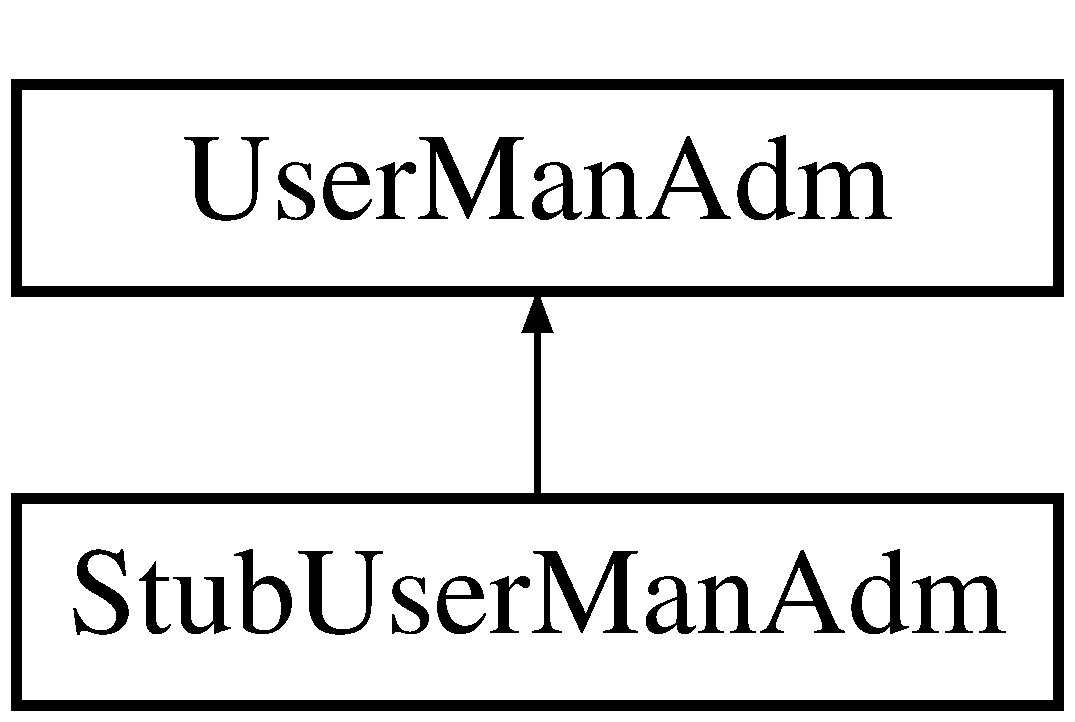
\includegraphics[height=2.000000cm]{dd/dfd/classStubUserManAdm}
\end{center}
\end{figure}
\subsection*{Public Member Functions}
\begin{DoxyCompactItemize}
\item 
\hypertarget{classStubUserManAdm_a63130507e95ab092b0bf09704b13b6ec}{void {\bfseries change\-Password} (\hyperlink{classUsrPassword}{Usr\-Password} $\ast$)  throw (\-Pers\-Error)}\label{dd/dfd/classStubUserManAdm_a63130507e95ab092b0bf09704b13b6ec}

\item 
\hypertarget{classStubUserManAdm_ac833e3729b1adf46edf78376719acde5}{void {\bfseries create\-Manager} (\hyperlink{classUsrName}{Usr\-Name} $\ast$, \hyperlink{classUsrPassword}{Usr\-Password} $\ast$)  throw (\-Pers\-Error)}\label{dd/dfd/classStubUserManAdm_ac833e3729b1adf46edf78376719acde5}

\item 
\hypertarget{classStubUserManAdm_a1d8b9e3691aef8438bf0b125efb54972}{list$<$ \hyperlink{classManager}{Manager} $\ast$ $>$ {\bfseries fetch\-Manager} (void)  throw (\-Pers\-Error)}\label{dd/dfd/classStubUserManAdm_a1d8b9e3691aef8438bf0b125efb54972}

\end{DoxyCompactItemize}


The documentation for this class was generated from the following files\-:\begin{DoxyCompactItemize}
\item 
User\-Unit.\-h\item 
User\-Unit.\-cpp\end{DoxyCompactItemize}

\hypertarget{classTest}{\section{Test$<$ info\-Type, class\-Type $>$ Class Template Reference}
\label{classTest}\index{Test$<$ info\-Type, class\-Type $>$@{Test$<$ info\-Type, class\-Type $>$}}
}


Template que irá gerar todas as classes de teste.  




{\ttfamily \#include $<$Test\-Unit.\-h$>$}

\subsection*{Public Member Functions}
\begin{DoxyCompactItemize}
\item 
\hypertarget{classTest_af4efb793913e8172ec96f64dd990b777}{void {\bfseries run} (const info\-Type \&, const info\-Type \&)}\label{classTest_af4efb793913e8172ec96f64dd990b777}

\end{DoxyCompactItemize}
\subsection*{Protected Attributes}
\begin{DoxyCompactItemize}
\item 
\hypertarget{classTest_ad228fd201d56aea9ebf26f7a5aefd2c1}{class\-Type $\ast$ {\bfseries object}}\label{classTest_ad228fd201d56aea9ebf26f7a5aefd2c1}

\end{DoxyCompactItemize}


\subsection{Detailed Description}
\subsubsection*{template$<$typename info\-Type, typename class\-Type$>$class Test$<$ info\-Type, class\-Type $>$}

Template que irá gerar todas as classes de teste. 

A partir desse template, todas as classes de teste podem ser modeladas, com seus respectivos métodos setup(), tear\-Down() e run(). 

The documentation for this class was generated from the following file\-:\begin{DoxyCompactItemize}
\item 
Test\-Unit.\-h\end{DoxyCompactItemize}

\hypertarget{classTextual}{\section{Textual Class Reference}
\label{de/da3/classTextual}\index{Textual@{Textual}}
}
Inheritance diagram for Textual\-:\begin{figure}[H]
\begin{center}
\leavevmode
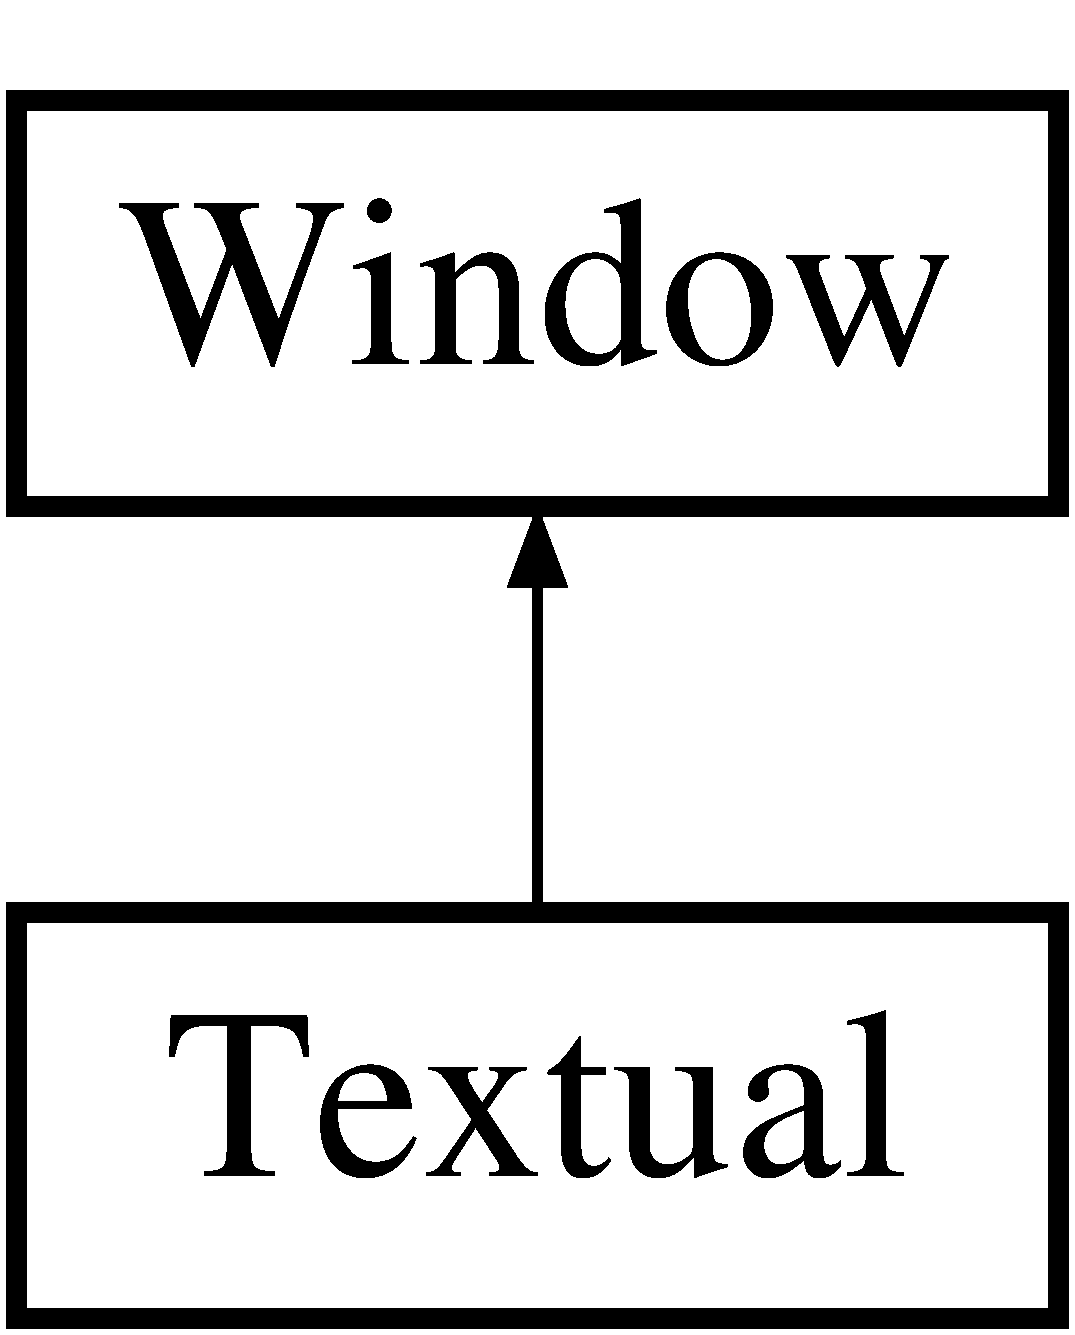
\includegraphics[height=2.000000cm]{de/da3/classTextual}
\end{center}
\end{figure}
\subsection*{Public Member Functions}
\begin{DoxyCompactItemize}
\item 
int \hyperlink{classTextual_a8b74c4f42ad3e8109ade0f12db4ccf3a}{menu} (int nopt, string options\mbox{[}$\,$\mbox{]}, string text)
\begin{DoxyCompactList}\small\item\em Mostra um menu de opções na tela. \end{DoxyCompactList}\item 
void \hyperlink{classTextual_a79264d4c405089034447a553cd3859e5}{print} (string)
\begin{DoxyCompactList}\small\item\em Mostra uma string na tela. \end{DoxyCompactList}\item 
void \hyperlink{classTextual_aab79476a2e99375655df0bc3d8738536}{print} (int)
\begin{DoxyCompactList}\small\item\em Mostra um inteiro na tela. \end{DoxyCompactList}\item 
void \hyperlink{classTextual_a5998864514acbf61ca8d6fa1845d0d22}{read} (string \&)
\begin{DoxyCompactList}\small\item\em Lê uma string da entrada padrão. \end{DoxyCompactList}\item 
void \hyperlink{classTextual_a888e02776648906696eeaea0e8691cd6}{read} (int \&)
\begin{DoxyCompactList}\small\item\em Lê um inteiro da entrada padrão. \end{DoxyCompactList}\item 
void \hyperlink{classTextual_a42ebc971370c4de20314ee33cd863cb3}{error} (string)
\begin{DoxyCompactList}\small\item\em Mostra a mensagem de erro formatada na tela. \end{DoxyCompactList}\item 
void \hyperlink{classTextual_ab9edde475ba8687ce2ed448212405e12}{success} (string)
\begin{DoxyCompactList}\small\item\em Mostra a mensagem de sucesso formatada na tela. \end{DoxyCompactList}\end{DoxyCompactItemize}


\subsection{Member Function Documentation}
\hypertarget{classTextual_a42ebc971370c4de20314ee33cd863cb3}{\index{Textual@{Textual}!error@{error}}
\index{error@{error}!Textual@{Textual}}
\subsubsection[{error}]{\setlength{\rightskip}{0pt plus 5cm}void Textual\-::error (
\begin{DoxyParamCaption}
\item[{string}]{}
\end{DoxyParamCaption}
)\hspace{0.3cm}{\ttfamily [virtual]}}}\label{de/da3/classTextual_a42ebc971370c4de20314ee33cd863cb3}


Mostra a mensagem de erro formatada na tela. 



Implements \hyperlink{classWindow_a2e661d42cd6e7b9c737530f4e34c87f1}{Window}.

\hypertarget{classTextual_a8b74c4f42ad3e8109ade0f12db4ccf3a}{\index{Textual@{Textual}!menu@{menu}}
\index{menu@{menu}!Textual@{Textual}}
\subsubsection[{menu}]{\setlength{\rightskip}{0pt plus 5cm}int Textual\-::menu (
\begin{DoxyParamCaption}
\item[{int}]{nopt, }
\item[{string}]{options\mbox{[}$\,$\mbox{]}, }
\item[{string}]{text}
\end{DoxyParamCaption}
)\hspace{0.3cm}{\ttfamily [virtual]}}}\label{de/da3/classTextual_a8b74c4f42ad3e8109ade0f12db4ccf3a}


Mostra um menu de opções na tela. 

Recebe um inteiro, o número de opções, e um vetor de strings, um vetor com o texto de cada uma das opções. 

Implements \hyperlink{classWindow_a3b6d7449c7f088f9ce59002573ca82c0}{Window}.

\hypertarget{classTextual_a79264d4c405089034447a553cd3859e5}{\index{Textual@{Textual}!print@{print}}
\index{print@{print}!Textual@{Textual}}
\subsubsection[{print}]{\setlength{\rightskip}{0pt plus 5cm}void Textual\-::print (
\begin{DoxyParamCaption}
\item[{string}]{}
\end{DoxyParamCaption}
)\hspace{0.3cm}{\ttfamily [virtual]}}}\label{de/da3/classTextual_a79264d4c405089034447a553cd3859e5}


Mostra uma string na tela. 



Implements \hyperlink{classWindow_a4fd86bca046073b3429f221c2f3bb690}{Window}.

\hypertarget{classTextual_aab79476a2e99375655df0bc3d8738536}{\index{Textual@{Textual}!print@{print}}
\index{print@{print}!Textual@{Textual}}
\subsubsection[{print}]{\setlength{\rightskip}{0pt plus 5cm}void Textual\-::print (
\begin{DoxyParamCaption}
\item[{int}]{}
\end{DoxyParamCaption}
)\hspace{0.3cm}{\ttfamily [virtual]}}}\label{de/da3/classTextual_aab79476a2e99375655df0bc3d8738536}


Mostra um inteiro na tela. 



Implements \hyperlink{classWindow_aa0a1210e72a63332e49722f1f878ea94}{Window}.

\hypertarget{classTextual_a5998864514acbf61ca8d6fa1845d0d22}{\index{Textual@{Textual}!read@{read}}
\index{read@{read}!Textual@{Textual}}
\subsubsection[{read}]{\setlength{\rightskip}{0pt plus 5cm}void Textual\-::read (
\begin{DoxyParamCaption}
\item[{string \&}]{}
\end{DoxyParamCaption}
)\hspace{0.3cm}{\ttfamily [virtual]}}}\label{de/da3/classTextual_a5998864514acbf61ca8d6fa1845d0d22}


Lê uma string da entrada padrão. 

Para ler senhas usando ($\ast$), definir password = true. Em outros casos, é possível suprimir este argumento. 

Implements \hyperlink{classWindow_abb59602c637907250fd70b1450b85c5c}{Window}.

\hypertarget{classTextual_a888e02776648906696eeaea0e8691cd6}{\index{Textual@{Textual}!read@{read}}
\index{read@{read}!Textual@{Textual}}
\subsubsection[{read}]{\setlength{\rightskip}{0pt plus 5cm}void Textual\-::read (
\begin{DoxyParamCaption}
\item[{int \&}]{}
\end{DoxyParamCaption}
)\hspace{0.3cm}{\ttfamily [virtual]}}}\label{de/da3/classTextual_a888e02776648906696eeaea0e8691cd6}


Lê um inteiro da entrada padrão. 



Implements \hyperlink{classWindow_ab00a4c057aade6ddc2a4bb22b2a6de42}{Window}.

\hypertarget{classTextual_ab9edde475ba8687ce2ed448212405e12}{\index{Textual@{Textual}!success@{success}}
\index{success@{success}!Textual@{Textual}}
\subsubsection[{success}]{\setlength{\rightskip}{0pt plus 5cm}void Textual\-::success (
\begin{DoxyParamCaption}
\item[{string}]{}
\end{DoxyParamCaption}
)\hspace{0.3cm}{\ttfamily [virtual]}}}\label{de/da3/classTextual_ab9edde475ba8687ce2ed448212405e12}


Mostra a mensagem de sucesso formatada na tela. 



Implements \hyperlink{classWindow_af625e87e68e0510c2fc11f1dc2d42f0e}{Window}.



The documentation for this class was generated from the following files\-:\begin{DoxyCompactItemize}
\item 
Engine\-Unit.\-h\item 
Engine\-Unit.\-cpp\end{DoxyCompactItemize}

\hypertarget{classTransacAdm}{\section{Transac\-Adm Class Reference}
\label{da/deb/classTransacAdm}\index{Transac\-Adm@{Transac\-Adm}}
}
Inheritance diagram for Transac\-Adm\-:\begin{figure}[H]
\begin{center}
\leavevmode
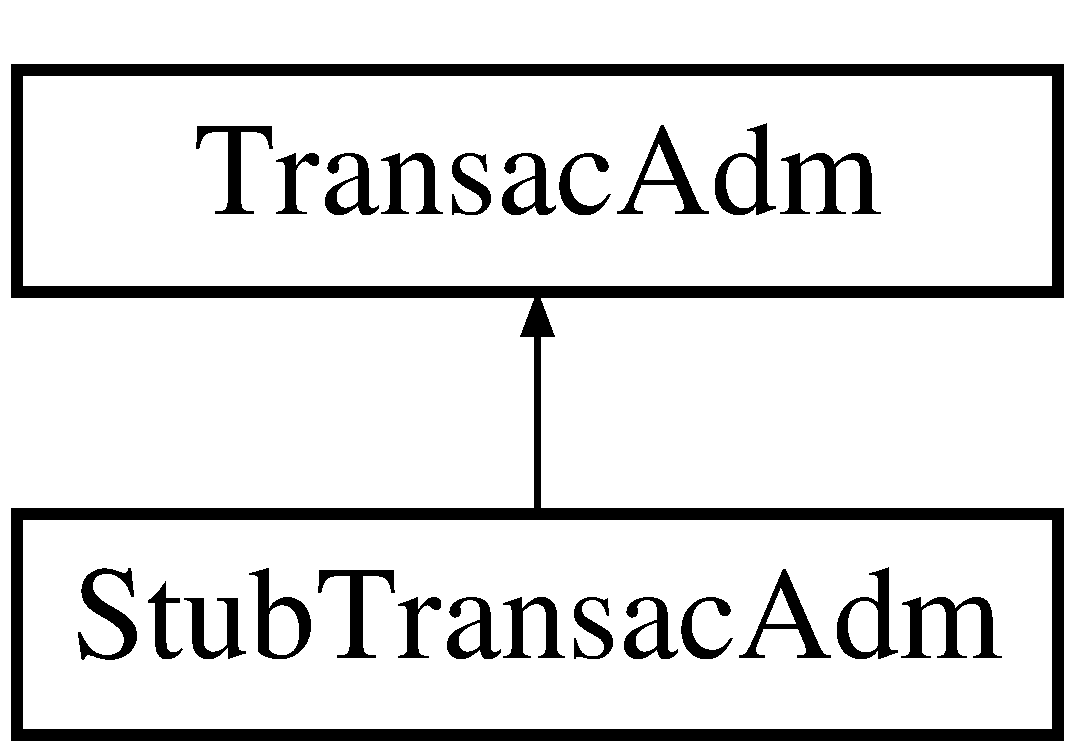
\includegraphics[height=2.000000cm]{da/deb/classTransacAdm}
\end{center}
\end{figure}
\subsection*{Public Member Functions}
\begin{DoxyCompactItemize}
\item 
\hypertarget{classTransacAdm_a128750caeeec2cd48a4a01e6ce9f701c}{virtual void {\bfseries withdraw} (\hyperlink{classAccNumber}{Acc\-Number}, \hyperlink{classMoney}{Money} $\ast$)=0  throw (invalid\-\_\-argument, Pers\-Error)}\label{da/deb/classTransacAdm_a128750caeeec2cd48a4a01e6ce9f701c}

\item 
\hypertarget{classTransacAdm_a9b6ffc8a521600094eb13510edcb33d7}{virtual void {\bfseries deposit} (\hyperlink{classAccNumber}{Acc\-Number}, \hyperlink{classMoney}{Money} $\ast$)=0  throw (invalid\-\_\-argument, Pers\-Error)}\label{da/deb/classTransacAdm_a9b6ffc8a521600094eb13510edcb33d7}

\end{DoxyCompactItemize}


The documentation for this class was generated from the following file\-:\begin{DoxyCompactItemize}
\item 
Transac\-Unit.\-h\end{DoxyCompactItemize}

\hypertarget{classUnitBase}{\section{Unit\-Base$<$ base\-Type $>$ Class Template Reference}
\label{d5/db5/classUnitBase}\index{Unit\-Base$<$ base\-Type $>$@{Unit\-Base$<$ base\-Type $>$}}
}


A base de derivação de todas as classes de tipos básicos.  




{\ttfamily \#include $<$Base\-Unit.\-h$>$}

\subsection*{Public Member Functions}
\begin{DoxyCompactItemize}
\item 
void \hyperlink{classUnitBase_a9cd392786b8078ab713045a8d1dece52}{set\-Value} (base\-Type \hyperlink{classUnitBase_a1c1ad08b45f07a94e5cf71dee734436b}{value})  throw (invalid\-\_\-argument)
\begin{DoxyCompactList}\small\item\em Método que define o valor do atributo value. \end{DoxyCompactList}\item 
base\-Type \hyperlink{classUnitBase_a6b4041c7176acb6c4956e085603449d1}{get\-Value} () const 
\begin{DoxyCompactList}\small\item\em Método que recupera o valor do atributo value. \end{DoxyCompactList}\end{DoxyCompactItemize}
\subsection*{Protected Attributes}
\begin{DoxyCompactItemize}
\item 
base\-Type \hyperlink{classUnitBase_a1c1ad08b45f07a94e5cf71dee734436b}{value}
\begin{DoxyCompactList}\small\item\em O valor comportado pela unidade. \end{DoxyCompactList}\end{DoxyCompactItemize}


\subsection{Detailed Description}
\subsubsection*{template$<$typename base\-Type$>$class Unit\-Base$<$ base\-Type $>$}

A base de derivação de todas as classes de tipos básicos. 

Suas diferentes instâncias servem de base para a construção de todos os outros tipos básicos. 

\subsection{Member Function Documentation}
\hypertarget{classUnitBase_a6b4041c7176acb6c4956e085603449d1}{\index{Unit\-Base@{Unit\-Base}!get\-Value@{get\-Value}}
\index{get\-Value@{get\-Value}!UnitBase@{Unit\-Base}}
\subsubsection[{get\-Value}]{\setlength{\rightskip}{0pt plus 5cm}template$<$typename base\-Type$>$ base\-Type {\bf Unit\-Base}$<$ base\-Type $>$\-::get\-Value (
\begin{DoxyParamCaption}
{}
\end{DoxyParamCaption}
) const\hspace{0.3cm}{\ttfamily [inline]}}}\label{d5/db5/classUnitBase_a6b4041c7176acb6c4956e085603449d1}


Método que recupera o valor do atributo value. 

O valor é retornado por este método, e o atributo não é modificado no processo. \hypertarget{classUnitBase_a9cd392786b8078ab713045a8d1dece52}{\index{Unit\-Base@{Unit\-Base}!set\-Value@{set\-Value}}
\index{set\-Value@{set\-Value}!UnitBase@{Unit\-Base}}
\subsubsection[{set\-Value}]{\setlength{\rightskip}{0pt plus 5cm}template$<$typename base\-Type$>$ void {\bf Unit\-Base}$<$ base\-Type $>$\-::set\-Value (
\begin{DoxyParamCaption}
\item[{base\-Type}]{value}
\end{DoxyParamCaption}
)  throw (invalid\-\_\-argument)\hspace{0.3cm}{\ttfamily [inline]}}}\label{d5/db5/classUnitBase_a9cd392786b8078ab713045a8d1dece52}


Método que define o valor do atributo value. 

A validação ocorre no processo, e o valor não será setado no caso do argumento deste método ser inválido. 

\subsection{Member Data Documentation}
\hypertarget{classUnitBase_a1c1ad08b45f07a94e5cf71dee734436b}{\index{Unit\-Base@{Unit\-Base}!value@{value}}
\index{value@{value}!UnitBase@{Unit\-Base}}
\subsubsection[{value}]{\setlength{\rightskip}{0pt plus 5cm}template$<$typename base\-Type$>$ base\-Type {\bf Unit\-Base}$<$ base\-Type $>$\-::value\hspace{0.3cm}{\ttfamily [protected]}}}\label{d5/db5/classUnitBase_a1c1ad08b45f07a94e5cf71dee734436b}


O valor comportado pela unidade. 

Seu tipo varia de acordo com a forma que o template é instanciado. 

The documentation for this class was generated from the following file\-:\begin{DoxyCompactItemize}
\item 
Base\-Unit.\-h\end{DoxyCompactItemize}

\hypertarget{classUser}{\subsection{User Class Reference}
\label{d9/dc0/classUser}\index{User@{User}}
}


Usuário; Base de derivação das classes \hyperlink{classCustomer}{Customer} e \hyperlink{classManager}{Manager}.  




{\ttfamily \#include $<$Entity\-Unit.\-h$>$}

Inheritance diagram for User\-:\begin{figure}[H]
\begin{center}
\leavevmode
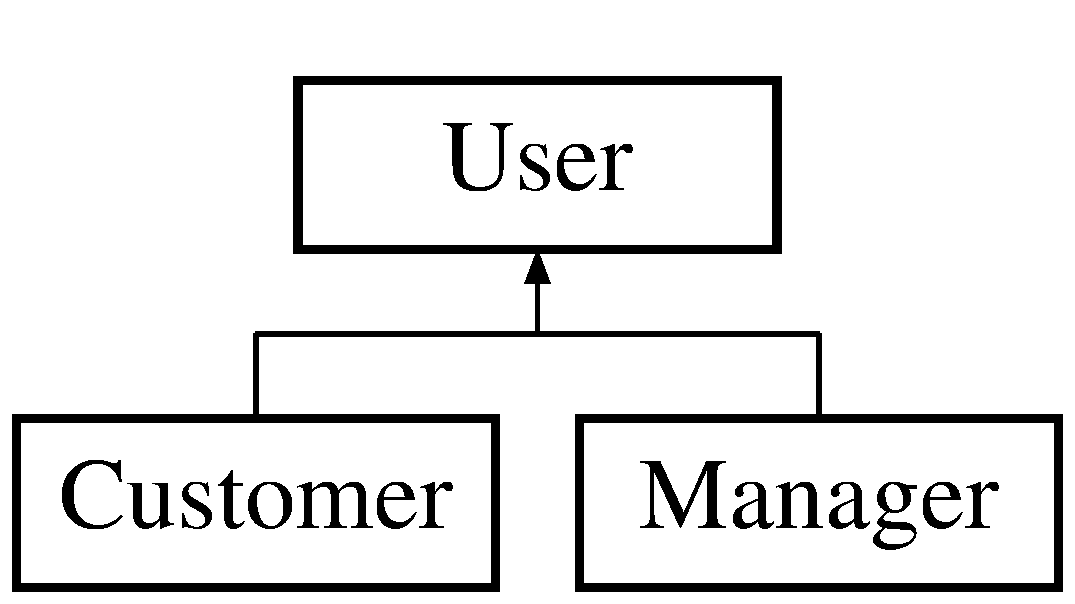
\includegraphics[height=2.000000cm]{d9/dc0/classUser}
\end{center}
\end{figure}
\subsubsection*{Public Member Functions}
\begin{DoxyCompactItemize}
\item 
\hyperlink{classUsrName}{Usr\-Name} \hyperlink{classUser_ae1dd9bb1a02ea1aa4246da19c28cd831}{get\-Name} () const 
\begin{DoxyCompactList}\small\item\em Método que recupera o valor contido no campo name. \end{DoxyCompactList}\item 
void \hyperlink{classUser_ac20aab332b1debfd3b94aa4fb7825b07}{set\-Usr\-Name} (const \hyperlink{classUsrName}{Usr\-Name} \&)
\begin{DoxyCompactList}\small\item\em Método que define o valor do atributo name. \end{DoxyCompactList}\item 
\hyperlink{classUsrPassword}{Usr\-Password} \hyperlink{classUser_a799c61fc6ff206a1b1edbc86d61989ed}{get\-Password} () const 
\begin{DoxyCompactList}\small\item\em Método que recupera o valor contido no campo password. \end{DoxyCompactList}\item 
void \hyperlink{classUser_ad36ece3d4decfd7f3db7f15c96eec99b}{set\-Usr\-Password} (const \hyperlink{classUsrPassword}{Usr\-Password} \&)
\begin{DoxyCompactList}\small\item\em Método que define o valor do atributo password. \end{DoxyCompactList}\end{DoxyCompactItemize}
\subsubsection*{Protected Attributes}
\begin{DoxyCompactItemize}
\item 
\hyperlink{classUsrName}{Usr\-Name} \hyperlink{classUser_a578e38a0fc23375ce19d689f96c6abaa}{name}
\begin{DoxyCompactList}\small\item\em Nome do usuário em questão. \end{DoxyCompactList}\item 
\hyperlink{classUsrPassword}{Usr\-Password} \hyperlink{classUser_a84c5ed822199a90e753ebfc54262fde8}{password}
\begin{DoxyCompactList}\small\item\em Senha do usuário em questão. \end{DoxyCompactList}\end{DoxyCompactItemize}


\subsubsection{Detailed Description}
Usuário; Base de derivação das classes \hyperlink{classCustomer}{Customer} e \hyperlink{classManager}{Manager}. 

Herdam dessa classe as duas maiores classes de usuários do sistema, os Clientes e os Gerentes. 

Definition at line 9 of file Entity\-Unit.\-h.



\subsubsection{Member Function Documentation}
\hypertarget{classUser_ae1dd9bb1a02ea1aa4246da19c28cd831}{\index{User@{User}!get\-Name@{get\-Name}}
\index{get\-Name@{get\-Name}!User@{User}}
\paragraph[{get\-Name}]{\setlength{\rightskip}{0pt plus 5cm}{\bf Usr\-Name} User\-::get\-Name (
\begin{DoxyParamCaption}
{}
\end{DoxyParamCaption}
) const\hspace{0.3cm}{\ttfamily [inline]}}}\label{d9/dc0/classUser_ae1dd9bb1a02ea1aa4246da19c28cd831}


Método que recupera o valor contido no campo name. 

O valor é retornado, e o atributo não é modificado no processo. 

Definition at line 29 of file Entity\-Unit.\-h.

\hypertarget{classUser_a799c61fc6ff206a1b1edbc86d61989ed}{\index{User@{User}!get\-Password@{get\-Password}}
\index{get\-Password@{get\-Password}!User@{User}}
\paragraph[{get\-Password}]{\setlength{\rightskip}{0pt plus 5cm}{\bf Usr\-Password} User\-::get\-Password (
\begin{DoxyParamCaption}
{}
\end{DoxyParamCaption}
) const\hspace{0.3cm}{\ttfamily [inline]}}}\label{d9/dc0/classUser_a799c61fc6ff206a1b1edbc86d61989ed}


Método que recupera o valor contido no campo password. 

O valor é retornado, e o atributo não é modificado no processo. 

Definition at line 33 of file Entity\-Unit.\-h.

\hypertarget{classUser_ac20aab332b1debfd3b94aa4fb7825b07}{\index{User@{User}!set\-Usr\-Name@{set\-Usr\-Name}}
\index{set\-Usr\-Name@{set\-Usr\-Name}!User@{User}}
\paragraph[{set\-Usr\-Name}]{\setlength{\rightskip}{0pt plus 5cm}void User\-::set\-Usr\-Name (
\begin{DoxyParamCaption}
\item[{const {\bf Usr\-Name} \&}]{name}
\end{DoxyParamCaption}
)}}\label{d9/dc0/classUser_ac20aab332b1debfd3b94aa4fb7825b07}


Método que define o valor do atributo name. 



Definition at line 7 of file Entity\-Unit.\-cpp.

\hypertarget{classUser_ad36ece3d4decfd7f3db7f15c96eec99b}{\index{User@{User}!set\-Usr\-Password@{set\-Usr\-Password}}
\index{set\-Usr\-Password@{set\-Usr\-Password}!User@{User}}
\paragraph[{set\-Usr\-Password}]{\setlength{\rightskip}{0pt plus 5cm}void User\-::set\-Usr\-Password (
\begin{DoxyParamCaption}
\item[{const {\bf Usr\-Password} \&}]{password}
\end{DoxyParamCaption}
)}}\label{d9/dc0/classUser_ad36ece3d4decfd7f3db7f15c96eec99b}


Método que define o valor do atributo password. 



Definition at line 11 of file Entity\-Unit.\-cpp.



\subsubsection{Member Data Documentation}
\hypertarget{classUser_a578e38a0fc23375ce19d689f96c6abaa}{\index{User@{User}!name@{name}}
\index{name@{name}!User@{User}}
\paragraph[{name}]{\setlength{\rightskip}{0pt plus 5cm}{\bf Usr\-Name} User\-::name\hspace{0.3cm}{\ttfamily [protected]}}}\label{d9/dc0/classUser_a578e38a0fc23375ce19d689f96c6abaa}


Nome do usuário em questão. 



Definition at line 12 of file Entity\-Unit.\-h.

\hypertarget{classUser_a84c5ed822199a90e753ebfc54262fde8}{\index{User@{User}!password@{password}}
\index{password@{password}!User@{User}}
\paragraph[{password}]{\setlength{\rightskip}{0pt plus 5cm}{\bf Usr\-Password} User\-::password\hspace{0.3cm}{\ttfamily [protected]}}}\label{d9/dc0/classUser_a84c5ed822199a90e753ebfc54262fde8}


Senha do usuário em questão. 



Definition at line 14 of file Entity\-Unit.\-h.



The documentation for this class was generated from the following files\-:\begin{DoxyCompactItemize}
\item 
Entity\-Unit.\-h\item 
Entity\-Unit.\-cpp\end{DoxyCompactItemize}

\hypertarget{classUserAccAdm}{\subsection{User\-Acc\-Adm Class Reference}
\label{dd/d35/classUserAccAdm}\index{User\-Acc\-Adm@{User\-Acc\-Adm}}
}


Interface de interação da camada de apresentação com a camada de negócio responsável pela administração dos dados de Contas.  




{\ttfamily \#include $<$User\-Unit.\-h$>$}

Inheritance diagram for User\-Acc\-Adm\-:\begin{figure}[H]
\begin{center}
\leavevmode
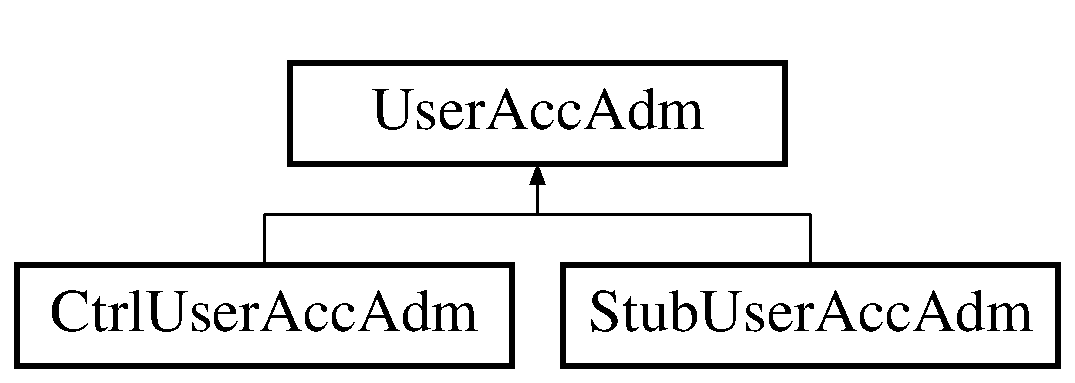
\includegraphics[height=2.000000cm]{dd/d35/classUserAccAdm}
\end{center}
\end{figure}
\subsubsection*{Public Member Functions}
\begin{DoxyCompactItemize}
\item 
virtual void \hyperlink{classUserAccAdm_a8bf3fc2dc45a1f13dbd8388cc37a26a2}{create\-Account} (\hyperlink{classUsrType}{Acc\-Type} $\ast$, \hyperlink{classMoney}{Money} $\ast$, \hyperlink{classMoney}{Money} $\ast$, \hyperlink{classUsrId}{Usr\-Id})=0  throw (\-Pers\-Error)
\begin{DoxyCompactList}\small\item\em Cria uma conta. \end{DoxyCompactList}\item 
virtual void \hyperlink{classUserAccAdm_a8257788e5e7d125b7482e490a6d71550}{delete\-Account} (\hyperlink{classAccNumber}{Acc\-Number} $\ast$)=0  throw (invalid\-\_\-argument, Pers\-Error)
\begin{DoxyCompactList}\small\item\em Deleta uma conta. \end{DoxyCompactList}\item 
virtual void \hyperlink{classUserAccAdm_ad9cdd01395ad7dd1b2c0887fe12b71b8}{block\-Account} (\hyperlink{classAccNumber}{Acc\-Number} $\ast$)=0  throw (invalid\-\_\-argument, Pers\-Error)
\begin{DoxyCompactList}\small\item\em Bloqueia uma conta. \end{DoxyCompactList}\item 
virtual void \hyperlink{classUserAccAdm_ae179b3e21f336b325452eb3c0981b0d9}{unblock\-Account} (\hyperlink{classAccNumber}{Acc\-Number} $\ast$)=0  throw (invalid\-\_\-argument, Pers\-Error)
\begin{DoxyCompactList}\small\item\em Desbloqueia uma conta. \end{DoxyCompactList}\item 
virtual list$<$ \hyperlink{classAccount}{Account} $>$ \hyperlink{classUserAccAdm_aa84b9df92ad9e11b1d9c71e9350efdc7}{fetch\-Account} (void)=0  throw (\-Pers\-Error)
\begin{DoxyCompactList}\small\item\em Recupera uma lista com todas as contas registradas. \end{DoxyCompactList}\item 
virtual \hyperlink{classAccount}{Account} \hyperlink{classUserAccAdm_a5957dcbf58d30b171a6ca0967dacf2d9}{fetch\-Account} (\hyperlink{classAccNumber}{Acc\-Number})=0  throw (\-Pers\-Error)
\begin{DoxyCompactList}\small\item\em Recupera os dados da conta de uma conta em específico. \end{DoxyCompactList}\item 
virtual void \hyperlink{classUserAccAdm_a80d61347b448e3ae9bdca4e02e65bcd1}{edit\-Acc\-Type} (\hyperlink{classAccNumber}{Acc\-Number} $\ast$, \hyperlink{classUsrType}{Acc\-Type} $\ast$)=0  throw (invalid\-\_\-argument, Pers\-Error)
\begin{DoxyCompactList}\small\item\em Edita o tipo de um conta. \end{DoxyCompactList}\item 
virtual void \hyperlink{classUserAccAdm_a43f0bb580d63a9c782e8c83417562a17}{edit\-Acc\-Limit} (\hyperlink{classAccNumber}{Acc\-Number} $\ast$, \hyperlink{classMoney}{Money} $\ast$)=0  throw (invalid\-\_\-argument, Pers\-Error)
\begin{DoxyCompactList}\small\item\em Edita o Limite de uma conta. \end{DoxyCompactList}\end{DoxyCompactItemize}


\subsubsection{Detailed Description}
Interface de interação da camada de apresentação com a camada de negócio responsável pela administração dos dados de Contas. 

Definition at line 37 of file User\-Unit.\-h.



\subsubsection{Member Function Documentation}
\hypertarget{classUserAccAdm_ad9cdd01395ad7dd1b2c0887fe12b71b8}{\index{User\-Acc\-Adm@{User\-Acc\-Adm}!block\-Account@{block\-Account}}
\index{block\-Account@{block\-Account}!UserAccAdm@{User\-Acc\-Adm}}
\paragraph[{block\-Account}]{\setlength{\rightskip}{0pt plus 5cm}virtual void User\-Acc\-Adm\-::block\-Account (
\begin{DoxyParamCaption}
\item[{{\bf Acc\-Number} $\ast$}]{}
\end{DoxyParamCaption}
)  throw (invalid\-\_\-argument, {\bf Pers\-Error})\hspace{0.3cm}{\ttfamily [pure virtual]}}}\label{dd/d35/classUserAccAdm_ad9cdd01395ad7dd1b2c0887fe12b71b8}


Bloqueia uma conta. 



Implemented in \hyperlink{classStubUserAccAdm_ac13ca4505d670a7bbb7c75d01b41a6d7}{Stub\-User\-Acc\-Adm}, and \hyperlink{classCtrlUserAccAdm_a31433e164de26c03becbc04f57c029ea}{Ctrl\-User\-Acc\-Adm}.

\hypertarget{classUserAccAdm_a8bf3fc2dc45a1f13dbd8388cc37a26a2}{\index{User\-Acc\-Adm@{User\-Acc\-Adm}!create\-Account@{create\-Account}}
\index{create\-Account@{create\-Account}!UserAccAdm@{User\-Acc\-Adm}}
\paragraph[{create\-Account}]{\setlength{\rightskip}{0pt plus 5cm}virtual void User\-Acc\-Adm\-::create\-Account (
\begin{DoxyParamCaption}
\item[{{\bf Acc\-Type} $\ast$}]{, }
\item[{{\bf Money} $\ast$}]{, }
\item[{{\bf Money} $\ast$}]{, }
\item[{{\bf Usr\-Id}}]{}
\end{DoxyParamCaption}
)  throw ({\bf Pers\-Error})\hspace{0.3cm}{\ttfamily [pure virtual]}}}\label{dd/d35/classUserAccAdm_a8bf3fc2dc45a1f13dbd8388cc37a26a2}


Cria uma conta. 



Implemented in \hyperlink{classStubUserAccAdm_ad6104bb252dd2627c42b65c47d026021}{Stub\-User\-Acc\-Adm}, and \hyperlink{classCtrlUserAccAdm_aa08ff58074dc0cb37c4d878e04b34adc}{Ctrl\-User\-Acc\-Adm}.

\hypertarget{classUserAccAdm_a8257788e5e7d125b7482e490a6d71550}{\index{User\-Acc\-Adm@{User\-Acc\-Adm}!delete\-Account@{delete\-Account}}
\index{delete\-Account@{delete\-Account}!UserAccAdm@{User\-Acc\-Adm}}
\paragraph[{delete\-Account}]{\setlength{\rightskip}{0pt plus 5cm}virtual void User\-Acc\-Adm\-::delete\-Account (
\begin{DoxyParamCaption}
\item[{{\bf Acc\-Number} $\ast$}]{}
\end{DoxyParamCaption}
)  throw (invalid\-\_\-argument, {\bf Pers\-Error})\hspace{0.3cm}{\ttfamily [pure virtual]}}}\label{dd/d35/classUserAccAdm_a8257788e5e7d125b7482e490a6d71550}


Deleta uma conta. 



Implemented in \hyperlink{classStubUserAccAdm_a6e95d2e9e35d658e581742e2d5e2fb60}{Stub\-User\-Acc\-Adm}, and \hyperlink{classCtrlUserAccAdm_aff45f0827b96208a4ccd6ae22610c5e3}{Ctrl\-User\-Acc\-Adm}.

\hypertarget{classUserAccAdm_a43f0bb580d63a9c782e8c83417562a17}{\index{User\-Acc\-Adm@{User\-Acc\-Adm}!edit\-Acc\-Limit@{edit\-Acc\-Limit}}
\index{edit\-Acc\-Limit@{edit\-Acc\-Limit}!UserAccAdm@{User\-Acc\-Adm}}
\paragraph[{edit\-Acc\-Limit}]{\setlength{\rightskip}{0pt plus 5cm}virtual void User\-Acc\-Adm\-::edit\-Acc\-Limit (
\begin{DoxyParamCaption}
\item[{{\bf Acc\-Number} $\ast$}]{, }
\item[{{\bf Money} $\ast$}]{}
\end{DoxyParamCaption}
)  throw (invalid\-\_\-argument, {\bf Pers\-Error})\hspace{0.3cm}{\ttfamily [pure virtual]}}}\label{dd/d35/classUserAccAdm_a43f0bb580d63a9c782e8c83417562a17}


Edita o Limite de uma conta. 



Implemented in \hyperlink{classStubUserAccAdm_aecabe86701249ca43bf17b99425d778e}{Stub\-User\-Acc\-Adm}, and \hyperlink{classCtrlUserAccAdm_a91d3db6c6233065aff60cbc679116467}{Ctrl\-User\-Acc\-Adm}.

\hypertarget{classUserAccAdm_a80d61347b448e3ae9bdca4e02e65bcd1}{\index{User\-Acc\-Adm@{User\-Acc\-Adm}!edit\-Acc\-Type@{edit\-Acc\-Type}}
\index{edit\-Acc\-Type@{edit\-Acc\-Type}!UserAccAdm@{User\-Acc\-Adm}}
\paragraph[{edit\-Acc\-Type}]{\setlength{\rightskip}{0pt plus 5cm}virtual void User\-Acc\-Adm\-::edit\-Acc\-Type (
\begin{DoxyParamCaption}
\item[{{\bf Acc\-Number} $\ast$}]{, }
\item[{{\bf Acc\-Type} $\ast$}]{}
\end{DoxyParamCaption}
)  throw (invalid\-\_\-argument, {\bf Pers\-Error})\hspace{0.3cm}{\ttfamily [pure virtual]}}}\label{dd/d35/classUserAccAdm_a80d61347b448e3ae9bdca4e02e65bcd1}


Edita o tipo de um conta. 



Implemented in \hyperlink{classStubUserAccAdm_a87d5b9af315af47b0f47baf66f75d9f0}{Stub\-User\-Acc\-Adm}, and \hyperlink{classCtrlUserAccAdm_a76260af4ccd5301504a50adbead90129}{Ctrl\-User\-Acc\-Adm}.

\hypertarget{classUserAccAdm_aa84b9df92ad9e11b1d9c71e9350efdc7}{\index{User\-Acc\-Adm@{User\-Acc\-Adm}!fetch\-Account@{fetch\-Account}}
\index{fetch\-Account@{fetch\-Account}!UserAccAdm@{User\-Acc\-Adm}}
\paragraph[{fetch\-Account}]{\setlength{\rightskip}{0pt plus 5cm}virtual list$<${\bf Account}$>$ User\-Acc\-Adm\-::fetch\-Account (
\begin{DoxyParamCaption}
\item[{void}]{}
\end{DoxyParamCaption}
)  throw ({\bf Pers\-Error})\hspace{0.3cm}{\ttfamily [pure virtual]}}}\label{dd/d35/classUserAccAdm_aa84b9df92ad9e11b1d9c71e9350efdc7}


Recupera uma lista com todas as contas registradas. 



Implemented in \hyperlink{classStubUserAccAdm_a29ba751355628d3e3a7ef1596b9b5108}{Stub\-User\-Acc\-Adm}, and \hyperlink{classCtrlUserAccAdm_a42e34f0780b86f393c25010e693450c2}{Ctrl\-User\-Acc\-Adm}.

\hypertarget{classUserAccAdm_a5957dcbf58d30b171a6ca0967dacf2d9}{\index{User\-Acc\-Adm@{User\-Acc\-Adm}!fetch\-Account@{fetch\-Account}}
\index{fetch\-Account@{fetch\-Account}!UserAccAdm@{User\-Acc\-Adm}}
\paragraph[{fetch\-Account}]{\setlength{\rightskip}{0pt plus 5cm}virtual {\bf Account} User\-Acc\-Adm\-::fetch\-Account (
\begin{DoxyParamCaption}
\item[{{\bf Acc\-Number}}]{}
\end{DoxyParamCaption}
)  throw ({\bf Pers\-Error})\hspace{0.3cm}{\ttfamily [pure virtual]}}}\label{dd/d35/classUserAccAdm_a5957dcbf58d30b171a6ca0967dacf2d9}


Recupera os dados da conta de uma conta em específico. 



Implemented in \hyperlink{classStubUserAccAdm_a05a1719f0ebfe4a2a7aed81505c82aba}{Stub\-User\-Acc\-Adm}, and \hyperlink{classCtrlUserAccAdm_a94e2637bedec766614095eee44bc9f38}{Ctrl\-User\-Acc\-Adm}.

\hypertarget{classUserAccAdm_ae179b3e21f336b325452eb3c0981b0d9}{\index{User\-Acc\-Adm@{User\-Acc\-Adm}!unblock\-Account@{unblock\-Account}}
\index{unblock\-Account@{unblock\-Account}!UserAccAdm@{User\-Acc\-Adm}}
\paragraph[{unblock\-Account}]{\setlength{\rightskip}{0pt plus 5cm}virtual void User\-Acc\-Adm\-::unblock\-Account (
\begin{DoxyParamCaption}
\item[{{\bf Acc\-Number} $\ast$}]{}
\end{DoxyParamCaption}
)  throw (invalid\-\_\-argument, {\bf Pers\-Error})\hspace{0.3cm}{\ttfamily [pure virtual]}}}\label{dd/d35/classUserAccAdm_ae179b3e21f336b325452eb3c0981b0d9}


Desbloqueia uma conta. 



Implemented in \hyperlink{classStubUserAccAdm_ad21405e80f7a8a2ea6a094363d4819d4}{Stub\-User\-Acc\-Adm}, and \hyperlink{classCtrlUserAccAdm_ad129cb69fc2a73cfb40bd52063d4369e}{Ctrl\-User\-Acc\-Adm}.



The documentation for this class was generated from the following file\-:\begin{DoxyCompactItemize}
\item 
User\-Unit.\-h\end{DoxyCompactItemize}

\hypertarget{classUserCusAdm}{\subsection{User\-Cus\-Adm Class Reference}
\label{d1/d48/classUserCusAdm}\index{User\-Cus\-Adm@{User\-Cus\-Adm}}
}


Interface de interação entre a camada de apresentação e a camada de negócio responsável pela administração de dados de clientes.  




{\ttfamily \#include $<$User\-Unit.\-h$>$}

Inheritance diagram for User\-Cus\-Adm\-:\begin{figure}[H]
\begin{center}
\leavevmode
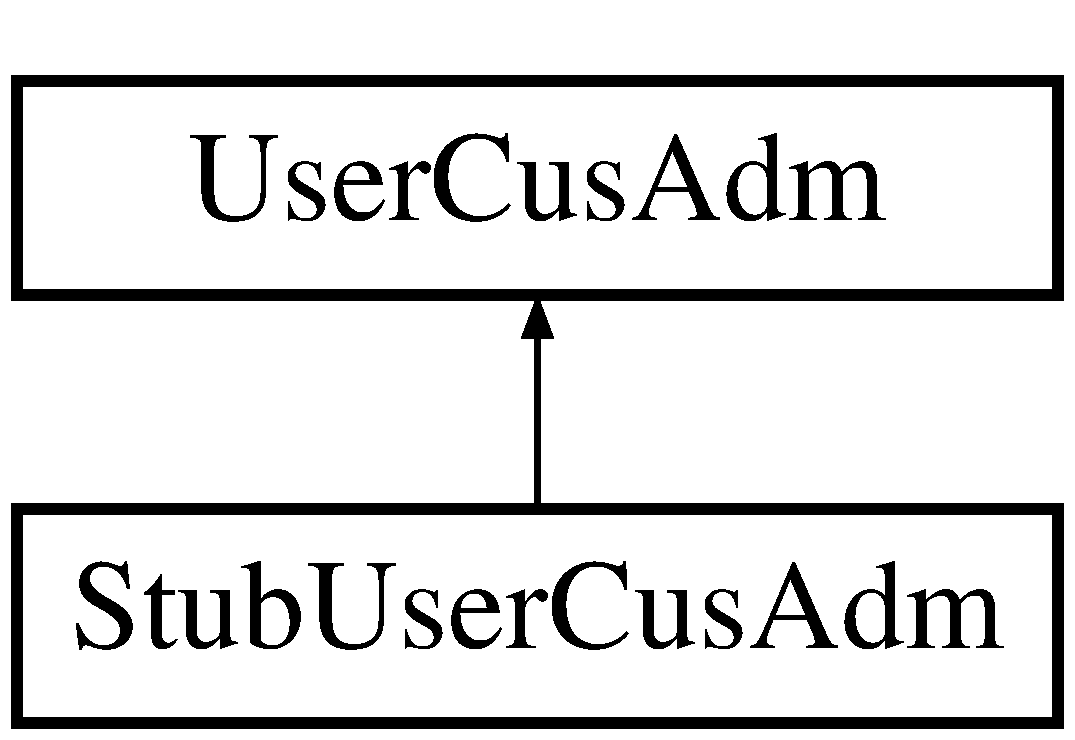
\includegraphics[height=2.000000cm]{d1/d48/classUserCusAdm}
\end{center}
\end{figure}
\subsubsection*{Public Member Functions}
\begin{DoxyCompactItemize}
\item 
virtual void \hyperlink{classUserCusAdm_aa78ba1b0eb4f14ca68f8ef2318e9c3d1}{change\-Password} (\hyperlink{classUsrPassword}{Usr\-Password} $\ast$)=0  throw (\-Pers\-Error)
\begin{DoxyCompactList}\small\item\em Modifica a senha do cliente. \end{DoxyCompactList}\item 
virtual \hyperlink{classUsrId}{Usr\-Id} \hyperlink{classUserCusAdm_a4775bb30caf44192349db204b95b2b2f}{create\-Customer} (\hyperlink{classUsrName}{Usr\-Name} $\ast$, \hyperlink{classUsrPassword}{Usr\-Password} $\ast$)=0  throw (invalid\-\_\-argument, Pers\-Error)
\begin{DoxyCompactList}\small\item\em Cria um cliente. \end{DoxyCompactList}\item 
virtual void \hyperlink{classUserCusAdm_a6105bcc548efb475bae0bc36b58743a2}{edit\-Cus\-Name} (\hyperlink{classAccNumber}{Acc\-Number} $\ast$, \hyperlink{classUsrName}{Usr\-Name} $\ast$)=0  throw (invalid\-\_\-argument, Pers\-Error)
\begin{DoxyCompactList}\small\item\em Edita o nome do cliente. \end{DoxyCompactList}\item 
virtual \hyperlink{classCustomer}{Customer} \hyperlink{classUserCusAdm_a8a67bf25c965e931be912f33449e0f8a}{fetch\-Customer} (\hyperlink{classUsrId}{Usr\-Id})=0  throw (\-Pers\-Error)
\begin{DoxyCompactList}\small\item\em Recupera so dados do cliente. \end{DoxyCompactList}\end{DoxyCompactItemize}


\subsubsection{Detailed Description}
Interface de interação entre a camada de apresentação e a camada de negócio responsável pela administração de dados de clientes. 



Definition at line 131 of file User\-Unit.\-h.



\subsubsection{Member Function Documentation}
\hypertarget{classUserCusAdm_aa78ba1b0eb4f14ca68f8ef2318e9c3d1}{\index{User\-Cus\-Adm@{User\-Cus\-Adm}!change\-Password@{change\-Password}}
\index{change\-Password@{change\-Password}!UserCusAdm@{User\-Cus\-Adm}}
\paragraph[{change\-Password}]{\setlength{\rightskip}{0pt plus 5cm}virtual void User\-Cus\-Adm\-::change\-Password (
\begin{DoxyParamCaption}
\item[{{\bf Usr\-Password} $\ast$}]{}
\end{DoxyParamCaption}
)  throw ({\bf Pers\-Error})\hspace{0.3cm}{\ttfamily [pure virtual]}}}\label{d1/d48/classUserCusAdm_aa78ba1b0eb4f14ca68f8ef2318e9c3d1}


Modifica a senha do cliente. 



Implemented in \hyperlink{classStubUserCusAdm_a7e44bec3dc4fb0640e6eb418dd8e8320}{Stub\-User\-Cus\-Adm}.

\hypertarget{classUserCusAdm_a4775bb30caf44192349db204b95b2b2f}{\index{User\-Cus\-Adm@{User\-Cus\-Adm}!create\-Customer@{create\-Customer}}
\index{create\-Customer@{create\-Customer}!UserCusAdm@{User\-Cus\-Adm}}
\paragraph[{create\-Customer}]{\setlength{\rightskip}{0pt plus 5cm}virtual {\bf Usr\-Id} User\-Cus\-Adm\-::create\-Customer (
\begin{DoxyParamCaption}
\item[{{\bf Usr\-Name} $\ast$}]{, }
\item[{{\bf Usr\-Password} $\ast$}]{}
\end{DoxyParamCaption}
)  throw (invalid\-\_\-argument, {\bf Pers\-Error})\hspace{0.3cm}{\ttfamily [pure virtual]}}}\label{d1/d48/classUserCusAdm_a4775bb30caf44192349db204b95b2b2f}


Cria um cliente. 



Implemented in \hyperlink{classStubUserCusAdm_a6b0c9fc7280045d06bf263d7286b37e9}{Stub\-User\-Cus\-Adm}.

\hypertarget{classUserCusAdm_a6105bcc548efb475bae0bc36b58743a2}{\index{User\-Cus\-Adm@{User\-Cus\-Adm}!edit\-Cus\-Name@{edit\-Cus\-Name}}
\index{edit\-Cus\-Name@{edit\-Cus\-Name}!UserCusAdm@{User\-Cus\-Adm}}
\paragraph[{edit\-Cus\-Name}]{\setlength{\rightskip}{0pt plus 5cm}virtual void User\-Cus\-Adm\-::edit\-Cus\-Name (
\begin{DoxyParamCaption}
\item[{{\bf Acc\-Number} $\ast$}]{, }
\item[{{\bf Usr\-Name} $\ast$}]{}
\end{DoxyParamCaption}
)  throw (invalid\-\_\-argument, {\bf Pers\-Error})\hspace{0.3cm}{\ttfamily [pure virtual]}}}\label{d1/d48/classUserCusAdm_a6105bcc548efb475bae0bc36b58743a2}


Edita o nome do cliente. 



Implemented in \hyperlink{classStubUserCusAdm_a84ca3047ccb0ac2e371a23c4e4fcdba0}{Stub\-User\-Cus\-Adm}.

\hypertarget{classUserCusAdm_a8a67bf25c965e931be912f33449e0f8a}{\index{User\-Cus\-Adm@{User\-Cus\-Adm}!fetch\-Customer@{fetch\-Customer}}
\index{fetch\-Customer@{fetch\-Customer}!UserCusAdm@{User\-Cus\-Adm}}
\paragraph[{fetch\-Customer}]{\setlength{\rightskip}{0pt plus 5cm}virtual {\bf Customer} User\-Cus\-Adm\-::fetch\-Customer (
\begin{DoxyParamCaption}
\item[{{\bf Usr\-Id}}]{}
\end{DoxyParamCaption}
)  throw ({\bf Pers\-Error})\hspace{0.3cm}{\ttfamily [pure virtual]}}}\label{d1/d48/classUserCusAdm_a8a67bf25c965e931be912f33449e0f8a}


Recupera so dados do cliente. 



Implemented in \hyperlink{classStubUserCusAdm_aac14b018a6284211b1c83c48a9529efe}{Stub\-User\-Cus\-Adm}.



The documentation for this class was generated from the following file\-:\begin{DoxyCompactItemize}
\item 
User\-Unit.\-h\end{DoxyCompactItemize}

\hypertarget{classUserLogin}{\subsection{User\-Login Class Reference}
\label{d4/de1/classUserLogin}\index{User\-Login@{User\-Login}}
}


Interface de interação da camada de apresentação com a camada de negócio responsável pelo login do usuário.  




{\ttfamily \#include $<$User\-Unit.\-h$>$}

Inheritance diagram for User\-Login\-:\begin{figure}[H]
\begin{center}
\leavevmode
\includegraphics[height=2.000000cm]{d4/de1/classUserLogin}
\end{center}
\end{figure}
\subsubsection*{Public Member Functions}
\begin{DoxyCompactItemize}
\item 
virtual \hyperlink{classUsrType}{Man\-Type} \hyperlink{classUserLogin_a15141f463faedae30e40115658fcc0b9}{autent} (\hyperlink{classUsrMatric}{Usr\-Matric} $\ast$, \hyperlink{classUsrPassword}{Usr\-Password} $\ast$)=0  throw (invalid\-\_\-argument, Pers\-Error)
\begin{DoxyCompactList}\small\item\em Autentica um administrador / gerente. \end{DoxyCompactList}\item 
virtual void \hyperlink{classUserLogin_a7163b2b97915fd0e3e5d3f76c2af44da}{autent} (\hyperlink{classAccNumber}{Acc\-Number} $\ast$, \hyperlink{classUsrPassword}{Usr\-Password} $\ast$)=0  throw (invalid\-\_\-argument, Pers\-Error)
\begin{DoxyCompactList}\small\item\em Autentica um cliente. \end{DoxyCompactList}\end{DoxyCompactItemize}


\subsubsection{Detailed Description}
Interface de interação da camada de apresentação com a camada de negócio responsável pelo login do usuário. 



Definition at line 11 of file User\-Unit.\-h.



\subsubsection{Member Function Documentation}
\hypertarget{classUserLogin_a15141f463faedae30e40115658fcc0b9}{\index{User\-Login@{User\-Login}!autent@{autent}}
\index{autent@{autent}!UserLogin@{User\-Login}}
\paragraph[{autent}]{\setlength{\rightskip}{0pt plus 5cm}virtual {\bf Man\-Type} User\-Login\-::autent (
\begin{DoxyParamCaption}
\item[{{\bf Usr\-Matric} $\ast$}]{, }
\item[{{\bf Usr\-Password} $\ast$}]{}
\end{DoxyParamCaption}
)  throw (invalid\-\_\-argument, {\bf Pers\-Error})\hspace{0.3cm}{\ttfamily [pure virtual]}}}\label{d4/de1/classUserLogin_a15141f463faedae30e40115658fcc0b9}


Autentica um administrador / gerente. 



Implemented in \hyperlink{classStubUserLogin_a9d84171d20e4e5dd9efb24cec9e61928}{Stub\-User\-Login}.

\hypertarget{classUserLogin_a7163b2b97915fd0e3e5d3f76c2af44da}{\index{User\-Login@{User\-Login}!autent@{autent}}
\index{autent@{autent}!UserLogin@{User\-Login}}
\paragraph[{autent}]{\setlength{\rightskip}{0pt plus 5cm}virtual void User\-Login\-::autent (
\begin{DoxyParamCaption}
\item[{{\bf Acc\-Number} $\ast$}]{, }
\item[{{\bf Usr\-Password} $\ast$}]{}
\end{DoxyParamCaption}
)  throw (invalid\-\_\-argument, {\bf Pers\-Error})\hspace{0.3cm}{\ttfamily [pure virtual]}}}\label{d4/de1/classUserLogin_a7163b2b97915fd0e3e5d3f76c2af44da}


Autentica um cliente. 



Implemented in \hyperlink{classStubUserLogin_a27bea5e442f63d62863ea4db5553d5cd}{Stub\-User\-Login}.



The documentation for this class was generated from the following file\-:\begin{DoxyCompactItemize}
\item 
User\-Unit.\-h\end{DoxyCompactItemize}

\hypertarget{classUserManAdm}{\section{User\-Man\-Adm Class Reference}
\label{da/d86/classUserManAdm}\index{User\-Man\-Adm@{User\-Man\-Adm}}
}
Inheritance diagram for User\-Man\-Adm\-:\begin{figure}[H]
\begin{center}
\leavevmode
\includegraphics[height=2.000000cm]{da/d86/classUserManAdm}
\end{center}
\end{figure}
\subsection*{Public Member Functions}
\begin{DoxyCompactItemize}
\item 
\hypertarget{classUserManAdm_a75006ea396a6384bbf47918fe9316bce}{virtual void {\bfseries change\-Password} (\hyperlink{classUsrPassword}{Usr\-Password} $\ast$)=0  throw (\-Pers\-Error)}\label{da/d86/classUserManAdm_a75006ea396a6384bbf47918fe9316bce}

\item 
\hypertarget{classUserManAdm_a4c1d61e8190867eb786cdf97083ba289}{virtual void {\bfseries create\-Manager} (\hyperlink{classUsrName}{Usr\-Name} $\ast$, \hyperlink{classUsrPassword}{Usr\-Password} $\ast$)=0  throw (\-Pers\-Error)}\label{da/d86/classUserManAdm_a4c1d61e8190867eb786cdf97083ba289}

\item 
\hypertarget{classUserManAdm_a05b8b4f5b1e42b7b9f77d6a40b90dbb2}{virtual list$<$ \hyperlink{classManager}{Manager} $>$ {\bfseries fetch\-Manager} (void)=0  throw (\-Pers\-Error)}\label{da/d86/classUserManAdm_a05b8b4f5b1e42b7b9f77d6a40b90dbb2}

\item 
\hypertarget{classUserManAdm_a62e826d1c11061df021016e94e88f9ba}{virtual \hyperlink{classManager}{Manager} {\bfseries fetch\-Manager} (\hyperlink{classUsrMatric}{Usr\-Matric})=0  throw (\-Pers\-Error)}\label{da/d86/classUserManAdm_a62e826d1c11061df021016e94e88f9ba}

\item 
\hypertarget{classUserManAdm_a0440de1c9d712a8dac1aa4e526d0fe9b}{virtual void {\bfseries edit\-Man\-Name} (\hyperlink{classUsrMatric}{Usr\-Matric} $\ast$, \hyperlink{classUsrName}{Usr\-Name} $\ast$)=0  throw (invalid\-\_\-argument, Pers\-Error)}\label{da/d86/classUserManAdm_a0440de1c9d712a8dac1aa4e526d0fe9b}

\item 
\hypertarget{classUserManAdm_a3fd6ddb6b71743fe5ece3100206023c3}{virtual void {\bfseries delete\-Manager} (\hyperlink{classUsrMatric}{Usr\-Matric} $\ast$)=0  throw (invalid\-\_\-argument, Pers\-Error)}\label{da/d86/classUserManAdm_a3fd6ddb6b71743fe5ece3100206023c3}

\end{DoxyCompactItemize}


The documentation for this class was generated from the following file\-:\begin{DoxyCompactItemize}
\item 
User\-Unit.\-h\end{DoxyCompactItemize}

\hypertarget{classUsrId}{\section{Usr\-Id Class Reference}
\label{d8/dc7/classUsrId}\index{Usr\-Id@{Usr\-Id}}
}


Define o I\-D de um \hyperlink{classCustomer}{Customer}.  




{\ttfamily \#include $<$Base\-Unit.\-h$>$}

Inheritance diagram for Usr\-Id\-:\begin{figure}[H]
\begin{center}
\leavevmode
\includegraphics[height=2.000000cm]{d8/dc7/classUsrId}
\end{center}
\end{figure}
\subsection*{Public Member Functions}
\begin{DoxyCompactItemize}
\item 
\hyperlink{classUsrId_a55a05b8f951a218c66c49f09fa6ce374}{Usr\-Id} ()
\begin{DoxyCompactList}\small\item\em Construtor padrão de \hyperlink{classUsrId}{Usr\-Id}. \end{DoxyCompactList}\item 
\hyperlink{classUsrId_a3be81b6f539c0121803f9d88e9d89553}{Usr\-Id} (const int \&)  throw (invalid\-\_\-argument)
\begin{DoxyCompactList}\small\item\em Construtor base de \hyperlink{classUsrId}{Usr\-Id}. \end{DoxyCompactList}\end{DoxyCompactItemize}
\subsection*{Additional Inherited Members}


\subsection{Detailed Description}
Define o I\-D de um \hyperlink{classCustomer}{Customer}. 

Tem a função de identificar de forma única um \hyperlink{classCustomer}{Customer}, independentemente do seu tipo de conta. 

\subsection{Constructor \& Destructor Documentation}
\hypertarget{classUsrId_a55a05b8f951a218c66c49f09fa6ce374}{\index{Usr\-Id@{Usr\-Id}!Usr\-Id@{Usr\-Id}}
\index{Usr\-Id@{Usr\-Id}!UsrId@{Usr\-Id}}
\subsubsection[{Usr\-Id}]{\setlength{\rightskip}{0pt plus 5cm}Usr\-Id\-::\-Usr\-Id (
\begin{DoxyParamCaption}
{}
\end{DoxyParamCaption}
)}}\label{d8/dc7/classUsrId_a55a05b8f951a218c66c49f09fa6ce374}


Construtor padrão de \hyperlink{classUsrId}{Usr\-Id}. 

Define o valor 0 como valor de não-\/inicialização deste tipo básico. \hypertarget{classUsrId_a3be81b6f539c0121803f9d88e9d89553}{\index{Usr\-Id@{Usr\-Id}!Usr\-Id@{Usr\-Id}}
\index{Usr\-Id@{Usr\-Id}!UsrId@{Usr\-Id}}
\subsubsection[{Usr\-Id}]{\setlength{\rightskip}{0pt plus 5cm}Usr\-Id\-::\-Usr\-Id (
\begin{DoxyParamCaption}
\item[{const int \&}]{usr\-Id}
\end{DoxyParamCaption}
)  throw (invalid\-\_\-argument)}}\label{d8/dc7/classUsrId_a3be81b6f539c0121803f9d88e9d89553}


Construtor base de \hyperlink{classUsrId}{Usr\-Id}. 

É preferível que se utilize este construtor, pois ele já faz a validação automática do valor a ser definido. 

The documentation for this class was generated from the following files\-:\begin{DoxyCompactItemize}
\item 
Base\-Unit.\-h\item 
Base\-Unit.\-cpp\end{DoxyCompactItemize}

\hypertarget{classUsrMatric}{\section{Usr\-Matric Class Reference}
\label{classUsrMatric}\index{Usr\-Matric@{Usr\-Matric}}
}


Define a matrícula de um \hyperlink{classManager}{Manager}.  




{\ttfamily \#include $<$Base\-Unit.\-h$>$}

Inheritance diagram for Usr\-Matric\-:\begin{figure}[H]
\begin{center}
\leavevmode
\includegraphics[height=2.000000cm]{classUsrMatric}
\end{center}
\end{figure}
\subsection*{Public Member Functions}
\begin{DoxyCompactItemize}
\item 
\hypertarget{classUsrMatric_acc7320dcfc8978fe9cc142340adb99c1}{{\bfseries Usr\-Matric} (const int \&)  throw (invalid\-\_\-argument)}\label{classUsrMatric_acc7320dcfc8978fe9cc142340adb99c1}

\end{DoxyCompactItemize}
\subsection*{Additional Inherited Members}


\subsection{Detailed Description}
Define a matrícula de um \hyperlink{classManager}{Manager}. 

Tem a função de identificar de forma única um \hyperlink{classManager}{Manager}, seja ele Administrador ou Gerente. 

The documentation for this class was generated from the following files\-:\begin{DoxyCompactItemize}
\item 
Base\-Unit.\-h\item 
Base\-Unit.\-cpp\end{DoxyCompactItemize}

\hypertarget{classUsrName}{\section{Usr\-Name Class Reference}
\label{da/df7/classUsrName}\index{Usr\-Name@{Usr\-Name}}
}


Define o nome de um \hyperlink{classUser}{User} (\hyperlink{classCustomer}{Customer} ou \hyperlink{classManager}{Manager}).  




{\ttfamily \#include $<$Base\-Unit.\-h$>$}

Inheritance diagram for Usr\-Name\-:\begin{figure}[H]
\begin{center}
\leavevmode
\includegraphics[height=2.000000cm]{da/df7/classUsrName}
\end{center}
\end{figure}
\subsection*{Public Member Functions}
\begin{DoxyCompactItemize}
\item 
\hyperlink{classUsrName_a0b0d5b9167309872d29c60a1946375af}{Usr\-Name} ()
\begin{DoxyCompactList}\small\item\em Construtor padrão de \hyperlink{classUsrName}{Usr\-Name}. \end{DoxyCompactList}\item 
\hyperlink{classUsrName_a3028672b21248ef880a01e3621e02827}{Usr\-Name} (const string \&)  throw (invalid\-\_\-argument)
\begin{DoxyCompactList}\small\item\em Construtor base de \hyperlink{classUsrName}{Usr\-Name}. \end{DoxyCompactList}\end{DoxyCompactItemize}
\subsection*{Additional Inherited Members}


\subsection{Detailed Description}
Define o nome de um \hyperlink{classUser}{User} (\hyperlink{classCustomer}{Customer} ou \hyperlink{classManager}{Manager}). 

Este tipo serve para regular o login de usuários em geral. 

\subsection{Constructor \& Destructor Documentation}
\hypertarget{classUsrName_a0b0d5b9167309872d29c60a1946375af}{\index{Usr\-Name@{Usr\-Name}!Usr\-Name@{Usr\-Name}}
\index{Usr\-Name@{Usr\-Name}!UsrName@{Usr\-Name}}
\subsubsection[{Usr\-Name}]{\setlength{\rightskip}{0pt plus 5cm}Usr\-Name\-::\-Usr\-Name (
\begin{DoxyParamCaption}
{}
\end{DoxyParamCaption}
)}}\label{da/df7/classUsrName_a0b0d5b9167309872d29c60a1946375af}


Construtor padrão de \hyperlink{classUsrName}{Usr\-Name}. 

Define a string vazia como valor de não-\/inicialização deste tipo básico \hypertarget{classUsrName_a3028672b21248ef880a01e3621e02827}{\index{Usr\-Name@{Usr\-Name}!Usr\-Name@{Usr\-Name}}
\index{Usr\-Name@{Usr\-Name}!UsrName@{Usr\-Name}}
\subsubsection[{Usr\-Name}]{\setlength{\rightskip}{0pt plus 5cm}Usr\-Name\-::\-Usr\-Name (
\begin{DoxyParamCaption}
\item[{const string \&}]{name}
\end{DoxyParamCaption}
)  throw (invalid\-\_\-argument)}}\label{da/df7/classUsrName_a3028672b21248ef880a01e3621e02827}


Construtor base de \hyperlink{classUsrName}{Usr\-Name}. 

É preferível que se utilize este construtor, pois ele já faz a validação automática do valor a ser definido. 

The documentation for this class was generated from the following files\-:\begin{DoxyCompactItemize}
\item 
Base\-Unit.\-h\item 
Base\-Unit.\-cpp\end{DoxyCompactItemize}

\hypertarget{classUsrPassword}{\section{Usr\-Password Class Reference}
\label{classUsrPassword}\index{Usr\-Password@{Usr\-Password}}
}


Define a senha de um \hyperlink{classUser}{User} (Customer ou \hyperlink{classManager}{Manager}).  




{\ttfamily \#include $<$Base\-Unit.\-h$>$}

Inheritance diagram for Usr\-Password\-:\begin{figure}[H]
\begin{center}
\leavevmode
\includegraphics[height=2.000000cm]{classUsrPassword}
\end{center}
\end{figure}
\subsection*{Public Member Functions}
\begin{DoxyCompactItemize}
\item 
\hypertarget{classUsrPassword_ab99c93719778f9560712675b1febb3cb}{{\bfseries Usr\-Password} (const string \&)  throw (invalid\-\_\-argument)}\label{classUsrPassword_ab99c93719778f9560712675b1febb3cb}

\end{DoxyCompactItemize}
\subsection*{Additional Inherited Members}


\subsection{Detailed Description}
Define a senha de um \hyperlink{classUser}{User} (Customer ou \hyperlink{classManager}{Manager}). 

Este tipo básico tem a função de controlar o login de usuários em geral. 

The documentation for this class was generated from the following files\-:\begin{DoxyCompactItemize}
\item 
Base\-Unit.\-h\item 
Base\-Unit.\-cpp\end{DoxyCompactItemize}

\hypertarget{classUsrType}{\subsection{Usr\-Type Class Reference}
\label{d1/dd4/classUsrType}\index{Usr\-Type@{Usr\-Type}}
}


Codifica tipos de conta.  




{\ttfamily \#include $<$Base\-Unit.\-h$>$}

Inheritance diagram for Usr\-Type\-:\begin{figure}[H]
\begin{center}
\leavevmode
\includegraphics[height=2.000000cm]{d1/dd4/classUsrType}
\end{center}
\end{figure}
\subsubsection*{Public Member Functions}
\begin{DoxyCompactItemize}
\item 
\hyperlink{classUsrType_a51a73c6f2cfbca3174120a2796957c03}{Usr\-Type} ()
\begin{DoxyCompactList}\small\item\em Construtor padrão de \hyperlink{classUsrType}{Usr\-Type}. \end{DoxyCompactList}\item 
\hyperlink{classUsrType_a774f3a391ac5741802862cb7de682bb9}{Usr\-Type} (const bool \&)  throw (invalid\-\_\-argument)
\begin{DoxyCompactList}\small\item\em Construtor base de \hyperlink{classUsrType}{Usr\-Type}. \end{DoxyCompactList}\end{DoxyCompactItemize}
\subsubsection*{Additional Inherited Members}


\subsubsection{Detailed Description}
Codifica tipos de conta. 

Possui duas utilizações\-: Acc\-Type\-: Codifica tipos de conta (Normal / Especial) Man\-Type\-: Codifica tipos de manager (Gerente / Administrador) 

Definition at line 120 of file Base\-Unit.\-h.



\subsubsection{Constructor \& Destructor Documentation}
\hypertarget{classUsrType_a51a73c6f2cfbca3174120a2796957c03}{\index{Usr\-Type@{Usr\-Type}!Usr\-Type@{Usr\-Type}}
\index{Usr\-Type@{Usr\-Type}!UsrType@{Usr\-Type}}
\paragraph[{Usr\-Type}]{\setlength{\rightskip}{0pt plus 5cm}Usr\-Type\-::\-Usr\-Type (
\begin{DoxyParamCaption}
{}
\end{DoxyParamCaption}
)}}\label{d1/dd4/classUsrType_a51a73c6f2cfbca3174120a2796957c03}


Construtor padrão de \hyperlink{classUsrType}{Usr\-Type}. 

Define o valor N\-O\-R\-M\-A\-L/\-G\-E\-R\-E\-N\-T\-E como valor de não-\/inicialização deste tipo básico. 

Definition at line 90 of file Base\-Unit.\-cpp.

\hypertarget{classUsrType_a774f3a391ac5741802862cb7de682bb9}{\index{Usr\-Type@{Usr\-Type}!Usr\-Type@{Usr\-Type}}
\index{Usr\-Type@{Usr\-Type}!UsrType@{Usr\-Type}}
\paragraph[{Usr\-Type}]{\setlength{\rightskip}{0pt plus 5cm}Usr\-Type\-::\-Usr\-Type (
\begin{DoxyParamCaption}
\item[{const bool \&}]{usr\-Type}
\end{DoxyParamCaption}
)  throw (invalid\-\_\-argument)}}\label{d1/dd4/classUsrType_a774f3a391ac5741802862cb7de682bb9}


Construtor base de \hyperlink{classUsrType}{Usr\-Type}. 

É preferível que se utilize este construtor, pois ele já faz a validação automática do valor a ser definido. 

Definition at line 95 of file Base\-Unit.\-cpp.



The documentation for this class was generated from the following files\-:\begin{DoxyCompactItemize}
\item 
Base\-Unit.\-h\item 
Base\-Unit.\-cpp\end{DoxyCompactItemize}

\hypertarget{classWindow}{\subsection{Window Class Reference}
\label{dc/dc4/classWindow}\index{Window@{Window}}
}


Responsável pela formatação de tela, entrada e saída básica.  




{\ttfamily \#include $<$Engine\-Unit.\-h$>$}

Inheritance diagram for Window\-:\begin{figure}[H]
\begin{center}
\leavevmode
\includegraphics[height=2.000000cm]{dc/dc4/classWindow}
\end{center}
\end{figure}
\subsubsection*{Public Member Functions}
\begin{DoxyCompactItemize}
\item 
virtual int \hyperlink{classWindow_a3b6d7449c7f088f9ce59002573ca82c0}{menu} (int nopt, string options\mbox{[}$\,$\mbox{]}, string text)=0
\begin{DoxyCompactList}\small\item\em Mostra um menu de opções na tela. \end{DoxyCompactList}\item 
virtual void \hyperlink{classWindow_a4fd86bca046073b3429f221c2f3bb690}{print} (string)=0
\begin{DoxyCompactList}\small\item\em Mostra uma string na tela. \end{DoxyCompactList}\item 
virtual void \hyperlink{classWindow_aa0a1210e72a63332e49722f1f878ea94}{print} (int)=0
\begin{DoxyCompactList}\small\item\em Mostra um inteiro na tela. \end{DoxyCompactList}\item 
virtual void \hyperlink{classWindow_a08f0e967158988de3cf9eb08a7823585}{print} (float)=0
\begin{DoxyCompactList}\small\item\em Mostra um float na tela. \end{DoxyCompactList}\item 
virtual void \hyperlink{classWindow_abb59602c637907250fd70b1450b85c5c}{read} (string \&)=0
\begin{DoxyCompactList}\small\item\em Lê uma string da entrada padrão. \end{DoxyCompactList}\item 
virtual void \hyperlink{classWindow_ab00a4c057aade6ddc2a4bb22b2a6de42}{read} (int \&)=0
\begin{DoxyCompactList}\small\item\em Lê um inteiro da entrada padrão. \end{DoxyCompactList}\item 
virtual void \hyperlink{classWindow_a2a1c43d55946185d0cee7324c78758fc}{read} (float \&)=0
\begin{DoxyCompactList}\small\item\em Lê um float da entrada padrão. \end{DoxyCompactList}\item 
virtual void \hyperlink{classWindow_a2e661d42cd6e7b9c737530f4e34c87f1}{error} (string)=0
\begin{DoxyCompactList}\small\item\em Mostra a mensagem de erro formatada na tela. \end{DoxyCompactList}\item 
virtual void \hyperlink{classWindow_af625e87e68e0510c2fc11f1dc2d42f0e}{success} (string)=0
\begin{DoxyCompactList}\small\item\em Mostra a mensagem de sucesso formatada na tela. \end{DoxyCompactList}\item 
virtual void \hyperlink{classWindow_ad7f70e7264c37772889b38ff4d82c68f}{pause} (void)=0
\begin{DoxyCompactList}\small\item\em Botão de continue. \end{DoxyCompactList}\end{DoxyCompactItemize}


\subsubsection{Detailed Description}
Responsável pela formatação de tela, entrada e saída básica. 



Definition at line 17 of file Engine\-Unit.\-h.



\subsubsection{Member Function Documentation}
\hypertarget{classWindow_a2e661d42cd6e7b9c737530f4e34c87f1}{\index{Window@{Window}!error@{error}}
\index{error@{error}!Window@{Window}}
\paragraph[{error}]{\setlength{\rightskip}{0pt plus 5cm}virtual void Window\-::error (
\begin{DoxyParamCaption}
\item[{string}]{}
\end{DoxyParamCaption}
)\hspace{0.3cm}{\ttfamily [pure virtual]}}}\label{dc/dc4/classWindow_a2e661d42cd6e7b9c737530f4e34c87f1}


Mostra a mensagem de erro formatada na tela. 



Implemented in \hyperlink{classTextual_a42ebc971370c4de20314ee33cd863cb3}{Textual}.

\hypertarget{classWindow_a3b6d7449c7f088f9ce59002573ca82c0}{\index{Window@{Window}!menu@{menu}}
\index{menu@{menu}!Window@{Window}}
\paragraph[{menu}]{\setlength{\rightskip}{0pt plus 5cm}virtual int Window\-::menu (
\begin{DoxyParamCaption}
\item[{int}]{nopt, }
\item[{string}]{options\mbox{[}$\,$\mbox{]}, }
\item[{string}]{text}
\end{DoxyParamCaption}
)\hspace{0.3cm}{\ttfamily [pure virtual]}}}\label{dc/dc4/classWindow_a3b6d7449c7f088f9ce59002573ca82c0}


Mostra um menu de opções na tela. 

Recebe um inteiro, o número de opções, e um vetor de strings, um vetor com o texto de cada uma das opções. 

Implemented in \hyperlink{classTextual_a8b74c4f42ad3e8109ade0f12db4ccf3a}{Textual}.

\hypertarget{classWindow_ad7f70e7264c37772889b38ff4d82c68f}{\index{Window@{Window}!pause@{pause}}
\index{pause@{pause}!Window@{Window}}
\paragraph[{pause}]{\setlength{\rightskip}{0pt plus 5cm}virtual void Window\-::pause (
\begin{DoxyParamCaption}
\item[{void}]{}
\end{DoxyParamCaption}
)\hspace{0.3cm}{\ttfamily [pure virtual]}}}\label{dc/dc4/classWindow_ad7f70e7264c37772889b38ff4d82c68f}


Botão de continue. 



Implemented in \hyperlink{classTextual_a2f7918232cd3b76ccf988bd41a622ec4}{Textual}.

\hypertarget{classWindow_a4fd86bca046073b3429f221c2f3bb690}{\index{Window@{Window}!print@{print}}
\index{print@{print}!Window@{Window}}
\paragraph[{print}]{\setlength{\rightskip}{0pt plus 5cm}virtual void Window\-::print (
\begin{DoxyParamCaption}
\item[{string}]{}
\end{DoxyParamCaption}
)\hspace{0.3cm}{\ttfamily [pure virtual]}}}\label{dc/dc4/classWindow_a4fd86bca046073b3429f221c2f3bb690}


Mostra uma string na tela. 



Implemented in \hyperlink{classTextual_a79264d4c405089034447a553cd3859e5}{Textual}.

\hypertarget{classWindow_aa0a1210e72a63332e49722f1f878ea94}{\index{Window@{Window}!print@{print}}
\index{print@{print}!Window@{Window}}
\paragraph[{print}]{\setlength{\rightskip}{0pt plus 5cm}virtual void Window\-::print (
\begin{DoxyParamCaption}
\item[{int}]{}
\end{DoxyParamCaption}
)\hspace{0.3cm}{\ttfamily [pure virtual]}}}\label{dc/dc4/classWindow_aa0a1210e72a63332e49722f1f878ea94}


Mostra um inteiro na tela. 



Implemented in \hyperlink{classTextual_aab79476a2e99375655df0bc3d8738536}{Textual}.

\hypertarget{classWindow_a08f0e967158988de3cf9eb08a7823585}{\index{Window@{Window}!print@{print}}
\index{print@{print}!Window@{Window}}
\paragraph[{print}]{\setlength{\rightskip}{0pt plus 5cm}virtual void Window\-::print (
\begin{DoxyParamCaption}
\item[{float}]{}
\end{DoxyParamCaption}
)\hspace{0.3cm}{\ttfamily [pure virtual]}}}\label{dc/dc4/classWindow_a08f0e967158988de3cf9eb08a7823585}


Mostra um float na tela. 



Implemented in \hyperlink{classTextual_a5558fc2f9db356453e60dbe6fc0e5dba}{Textual}.

\hypertarget{classWindow_abb59602c637907250fd70b1450b85c5c}{\index{Window@{Window}!read@{read}}
\index{read@{read}!Window@{Window}}
\paragraph[{read}]{\setlength{\rightskip}{0pt plus 5cm}virtual void Window\-::read (
\begin{DoxyParamCaption}
\item[{string \&}]{}
\end{DoxyParamCaption}
)\hspace{0.3cm}{\ttfamily [pure virtual]}}}\label{dc/dc4/classWindow_abb59602c637907250fd70b1450b85c5c}


Lê uma string da entrada padrão. 



Implemented in \hyperlink{classTextual_a5998864514acbf61ca8d6fa1845d0d22}{Textual}.

\hypertarget{classWindow_ab00a4c057aade6ddc2a4bb22b2a6de42}{\index{Window@{Window}!read@{read}}
\index{read@{read}!Window@{Window}}
\paragraph[{read}]{\setlength{\rightskip}{0pt plus 5cm}virtual void Window\-::read (
\begin{DoxyParamCaption}
\item[{int \&}]{}
\end{DoxyParamCaption}
)\hspace{0.3cm}{\ttfamily [pure virtual]}}}\label{dc/dc4/classWindow_ab00a4c057aade6ddc2a4bb22b2a6de42}


Lê um inteiro da entrada padrão. 



Implemented in \hyperlink{classTextual_a888e02776648906696eeaea0e8691cd6}{Textual}.

\hypertarget{classWindow_a2a1c43d55946185d0cee7324c78758fc}{\index{Window@{Window}!read@{read}}
\index{read@{read}!Window@{Window}}
\paragraph[{read}]{\setlength{\rightskip}{0pt plus 5cm}virtual void Window\-::read (
\begin{DoxyParamCaption}
\item[{float \&}]{}
\end{DoxyParamCaption}
)\hspace{0.3cm}{\ttfamily [pure virtual]}}}\label{dc/dc4/classWindow_a2a1c43d55946185d0cee7324c78758fc}


Lê um float da entrada padrão. 



Implemented in \hyperlink{classTextual_a2758b8a95187575114d49a528624b79d}{Textual}.

\hypertarget{classWindow_af625e87e68e0510c2fc11f1dc2d42f0e}{\index{Window@{Window}!success@{success}}
\index{success@{success}!Window@{Window}}
\paragraph[{success}]{\setlength{\rightskip}{0pt plus 5cm}virtual void Window\-::success (
\begin{DoxyParamCaption}
\item[{string}]{}
\end{DoxyParamCaption}
)\hspace{0.3cm}{\ttfamily [pure virtual]}}}\label{dc/dc4/classWindow_af625e87e68e0510c2fc11f1dc2d42f0e}


Mostra a mensagem de sucesso formatada na tela. 



Implemented in \hyperlink{classTextual_ab9edde475ba8687ce2ed448212405e12}{Textual}.



The documentation for this class was generated from the following file\-:\begin{DoxyCompactItemize}
\item 
Engine\-Unit.\-h\end{DoxyCompactItemize}

\addcontentsline{toc}{part}{Index}
\printindex
\end{document}
